\documentclass[11pt]{article}
\usepackage{amsmath} 
\usepackage{graphicx}
\usepackage{subcaption}
\usepackage{sectsty}
\usepackage{amssymb}
 \usepackage{lipsum}
\usepackage{titlesec}
\usepackage{romannum}
\usepackage{enumitem}
\usepackage{mathtools}
\usepackage[super]{nth}
\usepackage{tikz}
\usepackage{ragged2e}
\usepackage{pagecolor,lipsum}
\usepackage{float} % figure placement
\newcommand*\circled[1]{\tikz[baseline=(char.base)]{
            \node[shape=circle,draw,inner sep=2pt] (char) {#1};}}
\graphicspath{ {./images/} }
%Antiderivative Line
\DeclareMathOperator{\di}{d\!}
\newcommand*\Eval[3]{\left.#1\right\rvert_{#2}^{#3}}
\pagecolor{white}
\setlist[itemize,1]{leftmargin=\dimexpr 26pt-.5in}
%Set Equation Space above and Below
\setlength{\abovedisplayskip}{2pt}
\setlength{\belowdisplayskip}{2pt}


\sectionfont{\fontsize{12}{15}\selectfont}
\title{Introduction to Complex Analysis}
\author{Qitian Liao}
%\date{Aug 3, 2020} 
\usepackage[left=2cm, right=2cm, top=2cm]{geometry}
\setlength\parindent{0pt}

\DeclarePairedDelimiter\abs{\lvert}{\rvert}
\DeclarePairedDelimiter\norm{\lVert}{\rVert}

\begin{document}
%\pagenumbering{gobble}
\maketitle
\newpage
\tableofcontents
\def\Arg{\mathop{\operator@font Arg}\nolimits}
%\newpage
\pagenumbering{arabic}
\titleformat*{\section}{\Large\bfseries}
\titleformat*{\subsection}{\large\bfseries}
\titleformat*{\subsubsection}{\normalsize\bfseries}
\titleformat*{\paragraph}{\large\bfseries}
\titleformat*{\subparagraph}{\large\bfseries}

\titlespacing\section{0pt}{5pt plus 4pt minus 2pt}{5pt plus 2pt minus 2pt}
\titlespacing\subsection{0pt}{10pt plus 4pt minus 2pt}{5pt plus 2pt minus 2pt}
\titlespacing\subsubsection{0pt}{5pt plus 4pt minus 2pt}{5pt plus 2pt minus 2pt}

\newpage
\section{Algebra of the Complex Plane}
\subsection{Introduction to Complex Numbers}
\begin{figure}[H]
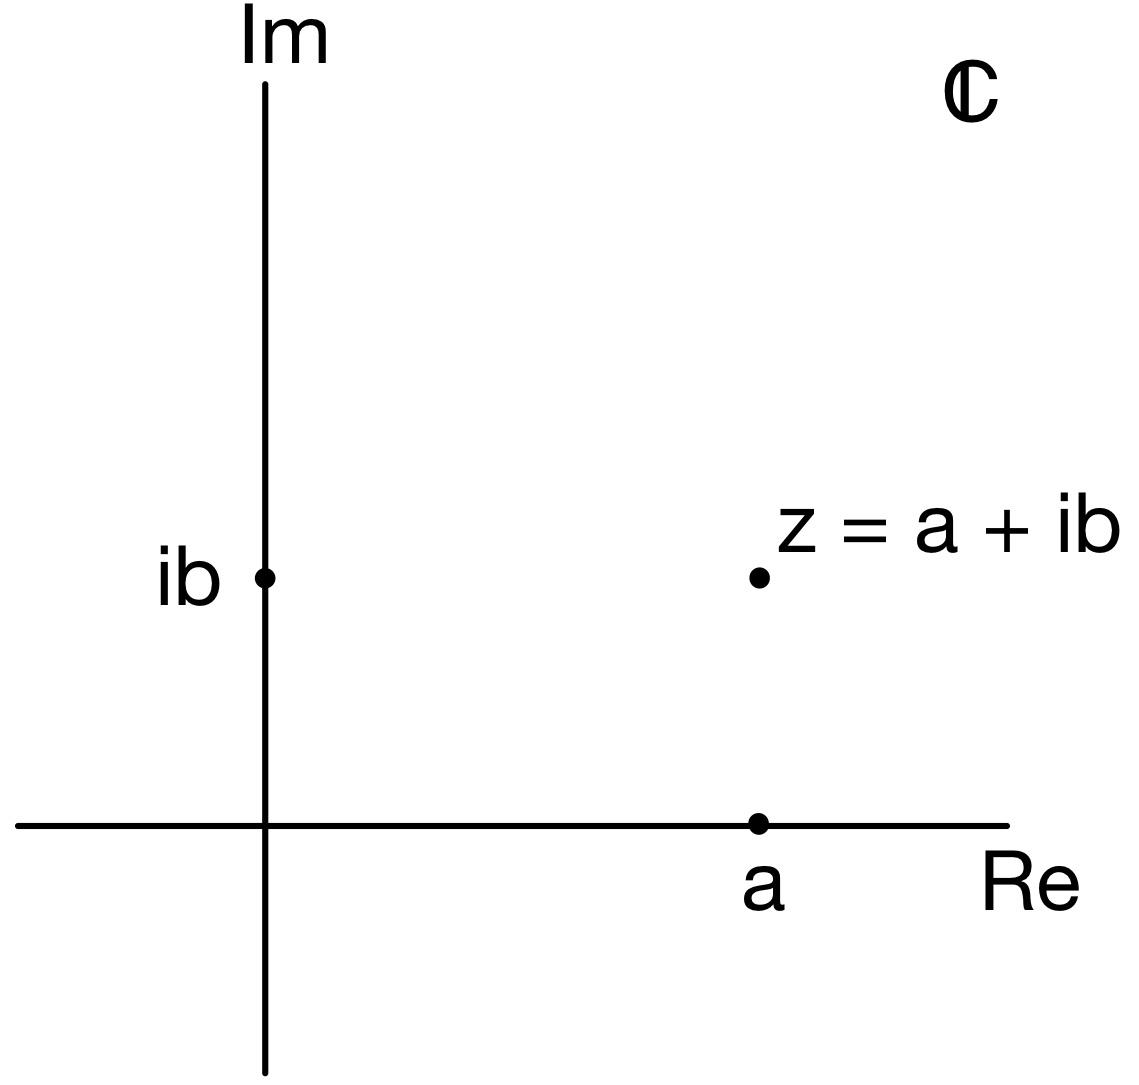
\includegraphics[scale = 0.15]{1_1}
\centering
\end{figure}
Let $z = a + ib \in \mathbb{C}$ where $a, b \in \mathbb{R}$ and $i ^ 2 = -1$. \\
This number can be thought of as a point in 2-space, $\mathbb{R} ^ 2$, $(a, b)$ or as a position in $\mathbb{C}$. \\ 
$\mathbb{R} ^ 2$: $\oplus$ addition; $\odot$ scalar multiplication. \\
$\mathbb{C}$ : $\oplus$ addition; $\odot$ scalar multiplication; a vector space; have multiplication of elements, $\mathbb{C}$ is a field. \\
\begin{equation*} 
\mbox{If } z = a + ib \mbox{, } w = c + id \mbox{, then }zw = (ac - bd) + i(ad + cb)
\end{equation*}
$$zw = wz$$
$$z(w + \alpha) = zw + z\alpha$$ 
$$(zw)\alpha = z(w\alpha)$$ 

\subsection{Conjugate of Complex Numbers} 
\newcommand*\conj[1]{\overline{#1}}
\textbf{Definition of Conjugate.} \\
The complex conjugate of $z$, $\conj{z}$, is defined by 
$$\conj{z} = a - ib$$ 
\begin{figure}[H]
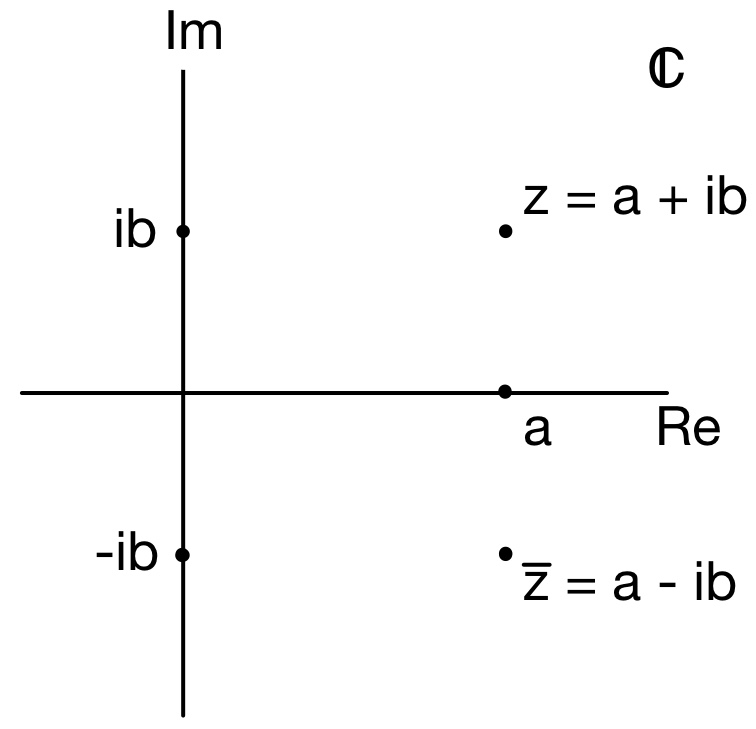
\includegraphics[scale = 0.19]{1_2}
\centering
\end{figure}
Geometric representation: The image of $\bar z$ is the reflection of z about the Real axis. \\
\newline
\textbf{Properties of Conjugate.} \\
$$\conj{\conj{z}} = z$$
$$\conj{zw} = \conj{z}\conj{w}$$
$$\conj{z + w} = \conj{z} + \conj{w}$$
\begin{equation*}
\overline{z} = z \mbox{ if and only if } z \in \mathbb{R}
\end{equation*}
\textbf{Real and Imaginary Parts.} \\
\newline
\noindent We can project $z$ onto the Real or Imaginary axis and measure its distance from 0: 
$$\Re(z) = a$$
\begin{equation*}
\Im(z) = b \mbox{, not } ib
\end{equation*}

Each function is a map $\mathbb{C} \to \mathbb{R}$. Then 
$$\Re(z) = \frac{z + \conj{z}}{2}$$
$$\Im(z) = \frac{z - \conj{z}}{2i}$$
This is similar to the pattern with even/odd functions. 

\subsection{Modulus of Complex Numbers.}
$z\conj{z} = (a + ib)(a - ib) = a^2 + b^2 \in \mathbb{R}$  \\

\textbf{Definition of Modulus.} \\
$|z|$ length/modulus of $z$ is defined by:
$$|z| = (a^2 + b^2)^{\frac{1}{2}} = (z\conj{z})^{\frac{1}{2}} \in \mathbb{R}$$
\begin{figure}[H]
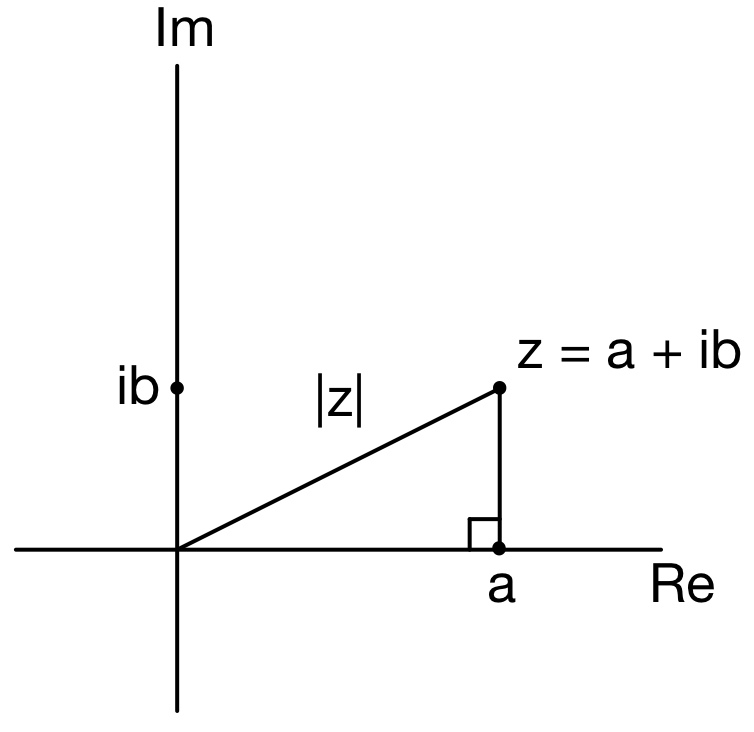
\includegraphics[scale = 0.19]{1_3}
\centering
\end{figure}
\textbf{Properties of Modulus.} \\
$$|zw| = |z||w|$$ 
$$|z| = |\conj{z}|$$  
$$|z| \geqslant 0$$
\begin{equation*}
|z| = 0 \mbox{ if and only if } z = 0
\end{equation*}
\newline
\textbf{Triangle Inequality and Reverse Triangle Inequality.} \\

\[ \begin{cases} 
      |z + w| \leqslant |z| + |w| \\
      |z| - |w| \leqslant |z - w|
   \end{cases}
\]

$$z = z - w + w \Rightarrow |z| = |z - w + w| \Rightarrow |z| \leqslant |z - w| + |w| \Rightarrow |z| - |w| \leqslant |z - w|$$
\newline
\textbf{Complex Division.} \\
With $z\conj{z} \in \mathbb{R}$, we can define complex division by reducing it to a multiplication problem. 
$$\frac{z}{w} = \frac{z\conj{w}}{w\conj{w}} = \frac{1}{w\conj{w}}(z\conj{w})$$ 
We also have 
\begin{equation*} 
\abs[\Big]{\frac{z}{w}} = \frac{|z|}{|w|} \mbox{ for } w \neq 0 
\end{equation*}

\textbf{Distance in the plane.} \\
A disk in the complex plane centered at $c$ of radius $r \in \mathbb{R}$ is of the form 
$$\{z \in \mathbb{C} \mid |z - c| \leqslant r\}$$
\\
\subsection{Complex Polynomial}
A complex polynomial $p(z)$ of degree n is of the form: 
$$p(z) = a_nz^n + a_{n - 1}z^{n - 1} + \cdots + a_1z + a_0$$
where $a_n \neq 0$ and $a_i \in \mathbb{C}$ for $ i = 0, \cdots , n$ \\
\newline
\textbf{Fundamental Theorem of Algebra.} \\

The factorization of $p(z)$ factors over $\mathbb{C}$ is unique, 
$$p(z) = c(z - z_1)^{m_1}...(z - z_k)^{m_k}$$
We have roots $z_i \in \mathbb{C}$ of $p(z)$ with order $m_i \in \mathbb{N}$. \\
For example, if $p(z) = z^2 + 4 = (z + 2i)(z - 2i)$, then it factors over $\mathbb{C}$ but not $\mathbb{R}$. \\
\textbf{Note}: 
$\mathbb{C}$ is an algebraically closed field, there are no irreducible polynomials in $\mathbb{C}$. \\
\textbf{Note}: 
$\mathbb{R}$,  $\mathbb{Q}$, $\mathbb{Z}$, $\mathbb{N}$ are not algebraically closed. \\

\newpage
\section{Geometry of the Complex Plane}
\subsection{Properties of Polar Forms} 
Complex numbers can be represented in polar forms: 
$$z = |z|(\cos\theta + i\sin\theta)$$
with modulus $|z|$ and argument $\theta$. To change between the coordinate systems it follows: 
$$|z| = (a^2 + b^2)^{\frac{1}{2}}$$
$$\tan\theta = \frac{b}{a}$$
$$a = |z|\cos\theta= \Re(z)$$
$$b = |z|\sin\theta = \Im(z)$$
Note that $\theta_R = \arctan(\frac{b}{a})$ is a reference angle of $z$. To find $\theta$ from $\theta_R$, you need to consider the signs of $a$ and $b$. \\
\newline
\textbf{Example.} \\
$$z = -3 + 3i = 3\sqrt2(\cos\frac{3\pi}{4} + \sin\frac{3\pi}{4})$$
$$\theta_R = \arctan(\frac{3}{-3})= -\frac{\pi}{4}$$
\begin{equation*}
\theta = \pi + \theta_R = \pi -\frac{\pi}{4} = \frac{3\pi}{4} \mbox{, since } \theta \mbox{ is in } \Romannum{2} .
\end{equation*}
\subsection{Definition of Argument and argument}
$\operatorname{Arg}(z)$ is $z$'s principle polar angle $\theta$, $z \neq 0$, where $\theta \in (-\pi, \pi]$. \\
$\operatorname{arg}(z)$ is all of $z$'s polar angles, $\theta + 2k\pi$, $k \in \mathbb{Z}$. 

\subsection{Euler's Formula} 
Euler's Formula is defined as a linear combination of $\cos\theta$ and $\sin\theta$, $\mathbb{R}$-valued functions. 
$$ e^{i\theta}= \cos\theta + i\sin\theta $$
It allows us to express $z$ in polar form by 
$$ z = |z|e^{i\theta}$$
-1 has polar angle $\pi$ and modulus 1, 
\begin{equation*}
-1 = e^{i\pi} \mbox{ or } e^{i\pi} + 1 = 0
\end{equation*}
By the angle addition formulas from trigonometry we find: 
$$e^{i\theta}e^{i\varphi} = e^{i(\theta + \varphi)}$$
$$(e^{i\theta})^k = e^{i\theta k}$$

\subsection{Geometric Understanding of Multiplication}
The polar angle of $zw$ is the sum of the polar angles of $z$ and $w$. The modulus is the product of the moduli. 
$$ \operatorname{Arg}(zw) = \operatorname{Arg}(z) + \operatorname{Arg}(w)$$
$$ \operatorname{Arg}(\conj{z}) = -\operatorname{Arg}(z)$$
Question: How about $\frac{z}{w}$ and $z^4$? \\
It follows from trigonometry that $|e^{i\theta}| = 1$, if $\theta \in (-\pi, \pi]$ we get a parametrization of the unit circle. \\
\newline
\textbf{Example.} Discover all solutions to $w^3 = i = z$ \\
Let $p(z) = w^3 - i$. By Fundamental Theorem of Algebra, there are 3 roots of $p(z)$. \\
Therefore, $3\theta= \frac{\pi}{2} + 2\pi k$, $k \in \mathbb{Z}$ \\
This gives us infinitely many solutions, but the solutions form 3 equivalence classes. \\
All we need is $k = 0, 1, 2$, which gives $\theta_1 = \frac{\pi}{6}$, $\theta_2 = \frac{5\pi}{6}$, $\theta_3 = \frac{3\pi}{2}$ \\
Our solutions partitioned the unit circle into 3 equally spaced wedges. \\
The solutions to $w^3 = i$ are $w_1 = \frac{\sqrt3}{2} + \frac{1}{2}i$, $w_2 = -\frac{\sqrt3}{2} + \frac{1}{2}i$ and $w_3 = -i$. \\
This problem of unity can be extended to solving $w^k = z$ for $k \in \mathbb{N}$, $z \in \mathbb{C}$ for unknown k-solutions w.  


\newpage
\section{Stereographic Projections, Exponentials and Logs}
\subsection{Stereographic Projections} 
We can express the complex plane on the unit sphere in $\mathbb{R}^3$. To perform this we project points on the surface of the sphere along the line from the North Pole $(0, 0, 1)$ through the point and onto the plane $z = 0, \mathbb{C}$ \\ 
$$p_1 = (x_1, x_2, x_3) \to z = a + ib = \frac{x_1 + ix_2}{1 - x_3}$$
$$x_1 = \frac{2a}{|z|^2 + 1}$$
$$x_2 = \frac{2b}{|z|^2 + 1}$$
$$x_3 = \frac{|z|^2 - 1}{|z|^2 + 1}$$
Points in the northern hemisphere $P_1$, have $|z_1| > 1$. \\
Points in the southern hemisphere $P_2$, have $|z_2| < 1$. \\
\newline
\textbf{Mapping from Stereographic Space to the Complex Plane.} 
\begin{align*}
\mathbb{S}^2 &\to \mathbb{C}\\
N = (0, 0, 1) &\to \infty \\
S = (0, 0, -1) &\to 0 \\
\mbox{lines of latitude } &\to |z| = r \mbox{, circles} \\
\mbox{lines of longitude } &\to \operatorname{Arg}(z) = \pm\theta \mbox{, lines through } (0, 0) 
\end{align*}
Note that in general, circles on $\mathbb{S}^2$ map to circles and lines in $\mathbb{C}$, orientation is not always preserved. 

\subsection{Complex Logarithm}
\textbf{Logarithm of Real Numbers.} \\
Anytime we are dealing with power, the log function is very useful. 
\begin{equation*}
\log{x} = \int_{1}^{x} \frac{1}{t} dt \mbox{ for } x \in \mathbb{R}
\end{equation*}
$$\frac{d}{dx}x^x = \frac{d}{dx}e^{\ln{x^x}} = \frac{d}{dx}e^{x\ln x} = e^{x\ln x}(x \cdot \frac{1}{x} + \ln{x}) = x^x(1 + \ln{x})$$
\newline
\textbf{Logarithm of Complex Numbers.} \\
Remember from Euler's Formula, $e^{i\theta}= \cos\theta + i\sin\theta$. 
$$e^z = e^{a + ib} = e^ae^{ib}$$ 
$$\operatorname{Arg}(e^z) = b$$
$$|e^z| = e^a > 0$$ 
Therefore, if $a$ is held fixed, $e^z$ maps to a circle as $b$ changes. \\
On the other hand, if $b$ is held fixed, $e^z$ maps to a line through $(0, 0)$. \\
\newline
\textbf{Derivation of Complex Logarithm.} \\
We want $e^{\log{(z)}} = z$ for all $z \neq 0$, and thus 
$$e^{\Re(\log{(z)}) + i\Im(\log{(z)})} = e^{\Re(\log{(z)})}e^{i\Im(\log{(z)})} = |z|e^{i\theta} = z$$
$$\Rightarrow |z| = e^{\Re(\log{(z)})}$$ 
$$\Rightarrow \Re(\log{(z)}) = \log{|z|}$$
From the imaginary part we find 
$$e^{i\theta} = e^{i\Im(\log{(z)})}$$
$$\Rightarrow \operatorname{arg}(z) = \theta = \Im(\log{(z)})$$
$$\Rightarrow \Im(\log{(z)}) = \operatorname{Arg}(z)$$ 
because $\operatorname{arg}(z)$ is not well defined. \\
Our constructed inverse of $e^z$ is a multi-valued function 
$$\log(z) = \log|z| + i\operatorname{arg}(z)$$
\newline
\textbf{Conclusion from Derivation.}\\
$$\log(z) = \log|z| + i\operatorname{arg}(z)$$
$$\operatorname{Log} (z) = \log|z| + i\operatorname{Arg}(z)$$
\textbf{Note}: $\operatorname{Log}(z)$ does not have all the nice behavior as $\mathbb{R}$-valued $\log(x)$: $\operatorname{Log}{(z^k)}$. \\
Sometimes they are co-terminal angles, but they are not equal. See the following example: \\
\[ \begin{cases} 
      \operatorname{Log}(i^3) = \operatorname{Log}(-i) = -i\frac{\pi}{2} \\
      3\operatorname{Log}(i) = 3 \cdot (i\frac{\pi}{2}) = i\frac{3\pi}{2}
   \end{cases}
\]
\textbf{Example.} Compute $3^i$: \\
$$3^i = e^{\operatorname{Log}{3^i}} = e^{i\operatorname{Log}{3}} = \cos{(\operatorname{Log}{3})} + i \sin{(\operatorname{Log}{3})}$$
\newline
\textbf{How Logarithm acts on curves. }\\
\[ \begin{cases} 
      \mbox{Maps a circle with radius } r \mbox{ to a vertical line passing through } (\ln(r), 0)\\
      \mbox{Maps a line with angle } \theta \mbox{ passing through the origin to a horizontal line passing through } (0, i\theta)
   \end{cases}
\]

\newpage
\section{Topology in $\mathbb{C}$}
\subsection{Sequence}
Let $\{Z_n\}$ be a sequence in $\mathbb{C}$. \\
\newline
\textbf{Cauchy Sequence. }\\
The sequence is Cauchy if for all $\varepsilon > 0$, there is a $N \in \mathbb{N}$ such that for all $n, m > N$, $|z_n - z_m| < \varepsilon$. \\
\newline
\textbf{Convergence of Sequence.}\\ 
The sequence converges if $|z_n - z| \to 0$ as $n \to \infty$. The distance between $z_n$ and $z$ vanishes. \\
\newline
\textbf{Completeness of $\mathbb{C}$.} \\
$\{z_n\}$ converges if and only if $\{z_n\}$ is Cauchy. \\
\textbf{Proof.} 
We show this by treating $\mathbb{C}$ as $\mathbb{R}^2$ and exploiting $\{X_n\}$ converges if and only if $\{X_n\}$ is Cauchy. \\
($\Longrightarrow$) (If $z_n \to z$, then $\Re(z_n) \to \Re(z)$ and $\Im(z_n) \to \Im(z)$. Since the sequences of $\mathbb{R}^2$ converge, they are Cauchy. \\
$|Z_n - Z_m| \leqslant |\Re(Z_n - Z_m)| +  |\Im(Z_n - Z_m)| = |\Re(Z_n) - \Re(Z_m)| + |\Im(Z_n) - \Im(Z_m)|$ \\
Upper bounds can be picked to be less than $\frac{\varepsilon}{2}$ for some $N$. Therefore, $|Z_n - Z_m| \to 0$. \\
\newline 
($\Longleftarrow$) If $\{Z_n\}$ is Cauchy, so are $\{\Re(Z_n)\}$ and $\{\Im(Z_n)\}$. But these are $\mathbb{R}$-sequences that converge. Therefore, $\{Z_n\}$ converges. 

\subsection{Complex Set} 
Let $\Omega \subset \mathbb{C}$. Sets can be open, closed, both, or neither. \\
\newline
\textbf{Open Set.} \\ 
If for any $z_0 \in \mathbb{C}$, there exist some $\varepsilon > 0$, such that the set $B_\varepsilon(z_0) = \{z||z - z_0| < \varepsilon\}$ is contained in $\Omega$, then $\Omega$ is open. \\
$\Omega$ is open if and only if $\Omega^c$ is closed. \\ 
$\Omega$ is open if and only if $\Omega$ is equal to its own interior, which means it does not contain its boundary points $\partial \Omega$, i.e. it does not contain its closure. \\
\newline
\textbf{Closed Set.} \\ 
If $\Omega$ contains its limit point, then $\Omega$ is closed. \\
$\Omega$ is closed if and only if $\Omega^c$ is open. \\ 
$\Omega$ is closed if and only if $\Omega$ contains its boundary points. \\
\newline
\textbf{Compact Set.}\\ 
If $\Omega$ can be contained in a disk of finite radius, then $\Omega$ is bounded. \\
\newline
\textbf{Compact Set.} \\ 
If $\Omega$ is closed and bounded, then $\Omega$ is compact. This resembles $[a, b]$ in $\mathbb{R}$. \\
\newline
\textbf{Connected Set.}\\ 
If any two points in $\Omega$ can be connected by a path, then $\Omega$ is connected. \\
\underline{Simply Connected Set}: A simply connected set has no "holes" in it. For example, $\Omega = \{z||z - c|<4\}$. \\
A connected but not simply connected set is an annulus, $\Omega = \{z|2< |z - c|<4\}$ \\
\newline
\textbf{Boundary of Set.}\\
The boundary of $\Omega$, $\partial \Omega$ is all points with $\varepsilon$-balls intersecting $\Omega$ and $\Omega^c$ for all $\varepsilon > 0$. \\
\newline
\textbf{Interior of Set.} \\
The interior of $\Omega$, Int$(\Omega)$, is all points in $\Omega$ with a $\varepsilon$-ball contained in $\Omega$ for some $\varepsilon > 0$. "Largest open set in $\Omega$". \\
\newline
\textbf{Closure of Set.} \\ 
The closure of $\Omega$ is the union of $\Omega$ and its boundary $\partial \Omega$. \\
\newline
\textbf{Domain.} \\
If a set is open and connected in $\mathbb{C}$, it is a domain. \\
A domain can be traversed by a path of horizontal and vertical line segments. \\
\newline
\textbf{Example.}\\
Determine whether the following sets are open or closed. 
\begin{enumerate}
  \item $\Omega = \mathbb{C} \backslash \{0\}$ \\
  $\Omega$ is open since it does not contain its closure, the point 0. \\
  $\Omega$ is not closed since it does not contain its limit points. Let $z_n = \frac{1}{n}$. Then $z_n = \frac{1}{n} \to 0 \notin \Omega$. \\
  Therefore, $\Omega$ is open. 
  \item $\Omega = \{z||z| \geqslant 1\}$ \\
  $\Omega$ is not open since any $\varepsilon$-ball at 1 intersects $\Omega^c$. \\
  $\Omega$ is closed since $\Omega^c$ is open. \\
  Therefore, $\Omega$ is closed. 
  \item $\Omega = \{z||z| > 1\}$ \\
  $\Omega$ is open since $\Omega^c$ is closed. \\
  $\Omega$ is not closed since it does not contain its limit points. Let $z_n = \frac{1}{n} + 1$. Then $z_n = \frac{1}{n} + 1 \to 1 \notin \Omega$.
  \item $\Omega = \mathbb{C} \backslash (0, 1)$ \\ 
  $\Omega$ is not open. Its complement is $[0, 1]$. Even though it is closed in $\mathbb{R}$, it is not closed in $\mathbb{C}$, because any 2D $\varepsilon$-ball will always extend outside of the set $z \in (0, i)$. Hence, $\Omega^c$ is not open and not closed. \\
  $\Omega$ is not closed since it does not contain its limit points. Let $z_n = \frac{1}{3} + i\frac{1}{n}$. Then $z_n = \frac{1}{3} + i\frac{1}{n} \to \frac{1}{3} \notin \Omega$. \\
  Therefore, $\Omega$ is neither open nor closed. 
  \item $\Omega = \mathbb{C} \backslash [0, 1]$
  $\Omega$ is open since $\Omega^c = [0, 1]$ is closed in $\mathbb{C}$. \\ 
  $\Omega$ is not closed since it does not contain its limit points. Let $z_n = \frac{1}{3} + i\frac{1}{n}$. Then $z_n = \frac{1}{3} + i\frac{1}{n} \to \frac{1}{3} \notin \Omega$. \\
  Therefore, $\Omega$ is open. \\ 
  Note: $\Omega^c$ is not open in $\mathbb{C}$. 
\end{enumerate}


\newpage
\section{Continuity and Branch Cuts}
\subsection{Complex Continuity} 
Let $f:\Omega \to \mathbb{C}$, $\Omega$ is open and connected. If $z_n \to z_0$ implies $f(z_n) \to f(z_0)$, then $f$ is continuous at $z_0$. Also, $f$ is bounded near $z_0$. \\
$f$ is continuous if for every $\varepsilon > 0$, there is $\delta > 0$ such that $|z - z_0| < \delta \Rightarrow |f(z) - f(z_0)| < \varepsilon$. \\
\newline 
In either case, $\Re(f(z))$ and $\Im(f(z))$ are each continuous if and only if $f(z)$ is continuous. This follows the pattern as $\mathbb{C}$ being complete. \\
\newline
If $f$ and $g$ are continuous, then so are $f + g$m $f \times g$ and $\frac{f}{g}$ (provided $g(z) \nrightarrow 0$)

\subsection{Complex Limits}
Just like in $\mathbb{R}^2$, limits are direction independent. Do not restrict limits to just $\Re \to 0$ or $\Im \to 0$. See the following example. \\
\begin{equation*}
\lim_{(x, y) \to (0, 0)} \frac{2x^2y}{x^4 + y^2} \mbox{ does not exist}
\end{equation*} 
as $x \to 0$, $y = 0$, then $f \to 0$, while $y = x^2, x \to 0$, then $f \to 1$.

\subsection{Branch Cuts}
$\operatorname{Log}$, $z^\frac{1}{2}$ and $\arctan(z)$ are constructed by restricting the range of $e^z$, $z^2$ and $\tan(z)$. \\
For example, in creating $\operatorname{Log}(z) = \ln|z| + i\operatorname{Arg}(z)$, we made a choice that $\operatorname{Arg}(z) \in (-\pi, \pi]$, $\operatorname{Arg}(0)$ does not exist. \\
\newline
\textbf{Example.} 
Consider a path around $z_0 \neq 0$, $\gamma(t) = z_0 + re^{it}$. $\theta(t) = \operatorname{arg}(\gamma(t))$. \\
As we traverse the circle, $t \in (-\pi, \pi]$, \\
$$\theta(t) = \operatorname{arg}(\gamma(t)) = \operatorname{Arg}(z_0 + re^{it}) + 2\pi k = \operatorname{Arg}(z_0 + re^{i(t + 2\pi)}) + 2\pi k = \operatorname{arg}(\gamma(t + 2\pi)) = \theta(t + 2\pi)$$
Therefore, the angle $\theta(t)$ changes smoothly for all $t$ and we stay on the same branch of $\operatorname{Arg}(\gamma(t))$. That is to say, the $k \in \mathbb{Z}$ is the same for all $t$.\\
\newline
Compare this with any circular path about $z = 0$, $\gamma_0$. Let $\gamma_0(t) = re^{it}$, $t \in (-\pi, \pi]$. As we traverse the circle once, we have a discontinuity in the principal angle of $\gamma_0(t)$. In particular, $\theta(\gamma_0(t)) \neq \theta(\gamma_0(t + 2\pi))$ \\
$$\theta(t) = \operatorname{arg}(\gamma(t)) = \operatorname{Arg}(re^{it}) + 2\pi k \neq \operatorname{Arg}(re^{i(t + 2\pi)}) + 2\pi (k + 1) = \operatorname{arg}(\gamma(t + 2\pi)) = \theta(t + 2\pi)$$
We jump from the $k$th to the $(k+1)$th branch of $\operatorname{Arg}$. Therefore, $\operatorname{Arg}(z)$ has a branch point at $z = 0$. \\

\textbf{Definition of Branch Cuts and Branch Points.}\\
If every neighborhood of $z_0$ contains a path $\gamma(t)$ around $z_0$ that leads to a jump discontinuity in $f$, then $z_0$ is a branch point of $f(z)$. \\ 
In order to find branches, at this point, it suffices to study paths of the form $\gamma(t) = z_0 + re^{it}$ for $t \in (-\pi, \pi)$, and see if $f(\gamma(t)) = f(\gamma(t + 2\pi))$ holds for all $t$. \\
\newline
\textbf{Example.} $\operatorname{Arg}$ is discontinuous for all $x$ on the negative $\mathbb{R}$-axis, $\mathbb{R}^-$. \\
We call this the principal branch cut of the multi-valued function $\operatorname{arg}$. Specifically, \\
\begin{equation*} 
\operatorname{Arg}(\gamma_0(t)) \to \pi \mbox{ as } t \to \pi^- 
\end{equation*}
\begin{equation*} 
\operatorname{Arg}(\gamma_0(t)) \to -\pi \mbox{ as } t \to -\pi^+
\end{equation*} 
but $\gamma_0(\pi) = \gamma_0(-\pi)$ since $\pi$ and $-\pi$ are coterminal. \\
$\mathbb{R}^-$ is the principal branch of $\operatorname{Log}$, $\operatorname{Arg}$, and $z^{\frac{1}{2}}$. \\
The endpoints of a branch cut are branch points, $\operatorname{Arg}$ has 0 and $\infty$ as its branch points. 

\newpage
\section{Differentiability in $\mathbb{C}$}
Let $f: \Omega \to \mathbb{C}$ for some domain $\Omega$. Then $f$ is differentiable at $z_0$ if the following exists. $$\frac{d}{dz}f(z)|_{z = z_0} = f'(z_0) = \lim_{h\to0}\frac{f(z + h) - f(z)}{h}$$
This limit must exist on all paths to $z_0$, since $h \in \mathbb{C}$. We could also take $z_n \to z_0$ and use $\frac{f(z_0) - f(z_n)}{z_0 - z_n} \to f'(z_0)$. 
Remember limits are computed by looking at the difference in the modulus, $|\frac{f(z_0) - f(z_n)}{z_0 - z_n} - f'(z_0)| \to 0$ as $n \to \infty$. \\
If $f'(z_0)$ exists on all points $z_0 \in \Omega$, open and connected in $\mathbb{C}$, then $f$ is holomorphic/$\mathbb{C}$-differentiable/analytic on $\Omega$. The connection between $\mathbb{R}$ and $\mathbb{C}$ analytic will be clear when we cover $\mathbb{C}$-power series. \\
If $f'(z)$ exists everywhere in $\mathbb{C}$, then $f$ is an entire/meromorphic function.  

\subsection{Difference between $\mathbb{R}$ and $\mathbb{C}$ differentiability}
$\bullet$ $f: \mathbb{R} \to \mathbb{R}$ 
$$\lim_{h\to0}\frac{f(x+h) - f(x)}{h} = f'(x)$$ 
has only two paths to $x$, namely $h \to 0^+$ and $h \to 0^-$. \\ 
Tangent plane or linear approximation: 
$$f(x) \approx f(a) + f'(a)(x - a)$$
$\bullet$ $f: \mathbb{R}^2 \to \mathbb{R}$
$$\lim_{h\to0}\frac{f(x+h, y) - f(x, y)}{h} = f_x$$ 
is also a 1D limit and a partial derivative. \\
Tangent plane or linear approximation: 
$$f(x,y) \approx f(a,b) + f_x(a,b)(x - a) + f_y(a, b)(y - b)$$
$\bullet$ $f: \mathbb{R}^2 \to \mathbb{R}^2$ $f(x, y) = (u(x, y),v(x,y))$ \\
Then $f$ is differentiable if the Jacobian Matrix
\begin{equation*}
J(f) = 
\begin{bmatrix}
 u_x & u_y \\
 v_x & v_y
\end{bmatrix}
\end{equation*}
can approximate the local change in $f$. \\
In each of the cases above, we are only measuring change in a few directions. However, $h \to0$ in $\mathbb{C}$ can be from any direction in 2-space. Therefore, $f'(z)$ existing is a much stronger condition for $f$ on $\mathbb{C}$ than on $\mathbb{R}$. \\
\newline
\textbf{Complications with $\conj{z}$.}\\
Consider the following example: \\
Let $g(z) = \Re(z) = \frac{z + \conj{z}}{2}$, which is a linear combination of continuous functions. \\
Assume $h \in \mathbb{R}$, 
\begin{equation*}
\frac{g(z + ih) - g(z)}{h} = \frac{\Re(z) - \Re(z)}{h} \to 0 \mbox{ as } h \to 0 
\end{equation*}
Compare this with 
\begin{equation*} 
\frac{g(z + ih) - g(z)}{h} = \frac{\Re(z) + h -\Re(z)}{h} = 1 \to 1 \mbox{ as } h \to 0
\end{equation*}
Therefore, the function is nowhere differentiable in $\mathbb{C}$. The problem with $g'(z)$ had to do with $\conj{z}$, despite reflection in $\mathbb{R}^2$ about $y = 0$ is differentiable. We will discover conditions on $u_x$, $u_y$, $v_x$, and $v_y$ that ensure $f'$ exists for $f(z) = u(x, y) + iv(x, y)$ in the next chapter.  \\

\subsection{Properties of $f'(z)$}
\textbf{Proposition.} If $f$ is differentiable on $\Omega$, it is continuous on $\Omega$. \\
\textbf{Proposition.} The power rule holds too: $\frac{d}{dz}z^n = nz^{z - 1}$\\
As does the product, quotient, L'Hospital's and chain rule. In fact, most old results hold as well. 
In each of the following cases, there are branch points where $f'(z)$ does not exist. \\
1. If $f(z) = \operatorname{Log}(z)$, then $f'(z) = \frac{1}{z}$ \\
2. If $f(z) = \tan^{-1}(z)$, then $f'(z) = \frac{1}{z^2 + 1} = \frac{1}{(z + i)(z - i)}$, which does not exist for $z = \pm i$ \\
3. If $f(z) = z^\frac{1}{2}$, then $f'(z) = \frac{1}{2}z^{-\frac{1}{2}}$ \\

\textbf{Proposition.} Suppose $f(z)$ is holomorphic on $\Omega$. then $g(z) = \conj{f(\conj{z})}$ is holomorphic on $\Omega^{\ast} = \{z|\conj{z} \in \Omega\}$ \\
\textbf{Proof.} Suppose $f$ is holomorphic on $\Omega$. Let $z_0 \in \Omega^{\ast}$ and $z_n \in \Omega^{\ast}$ for all $n$ and $z_n \to z$. Then $\conj{z_n} \to \conj{z_0}$ in $\Omega$ and for $\varepsilon > 0$, there is a $N \in \mathbb{N}$ such that for $n > N$. 
$$\abs*{\frac{f(\conj{z_0}) - f(\conj{z_n})}{\conj{z_0} - \conj{z_n}} - f'(\conj{z_0})} < \varepsilon$$ 
$$\abs*{\frac{f(\conj{z_0}) - f(\conj{z_n})}{\conj{z_0} - \conj{z_n}} - f'(\conj{z_0})} = \conj{\abs*{\frac{f(\conj{z_0}) - f(\conj{z_n})}{\conj{z_0} - \conj{z_n}} - f'(\conj{z_0})}} = \abs*{\frac{\conj{{f(\conj{z_0}) - f(\conj{z_n})}}}{\conj{\conj{z_0} - \conj{z_n}}} - \conj{f'(\conj{z_0})}} $$
$$ = \abs*{\frac{\conj{{f(\conj{z_0}) - f(\conj{z_n})}}}{z_0 - z_n} - \conj{f'(\conj{z_0})}} = \abs*{\frac{g(z_0) - g(z_n)}{z_0 - z_n} - \conj{f'(\conj{z_0})}} < \varepsilon$$
$$\Longrightarrow g'(z_0) = \conj{f'(\conj{z_0})}$$
Therefore, $g$ is holomorphic on $\Omega^\ast$. \\
This proof is different from when we showed $\frac{d}{dz}\conj{z}$ does not exist. Conjugation must be handled with care. 
%\abs[\Big]
\subsection{Geometric behavior of $f'(z)$}
\textbf{Dilation.}\\ 
$w = f(z) \approx f'(a)(z - a) + f(a)$. Small changes in $z$ should give small changes in $w$. \\
The functions $|z|$ and $\operatorname{Arg}(z)$ are continuous on their domains. \\
If $f'(z_0) \neq 0$ and $f'$ exists on $\Omega$, then 
$$ |f'(z_0)| = \abs*{\lim_{h \to 0}\frac{f(z_0 + h) - f(z_0)}{h}} = \lim_{h \to 0} \abs*{\frac{f(z_0 + h) - f(z_0)}{h}} = \lim_{h \to 0}\frac{|f(z_0 + h) - f(z_0)|}{|h|}$$
$$\Longrightarrow |f'(z_0)||h| \approx |f(z + h) - f(z)|$$
The size of $|f'(z_0)|$ tells us how much $f$ is contracting/dilating near $z_0$. \\
\newline
\textbf{Rotation.}\\
$$\operatorname{Arg}(f'(z_0)) = \operatorname{Arg}\left(\lim_{h \to 0}\frac{f(z_0 + h) - f(z_0)}{h}\right) = \lim_{h \to 0}\operatorname{Arg}\left(\frac{f(z_0 + h) - f(z)}{h}\right)$$
$$ = \lim_{h \to 0} \operatorname{Arg}(f(z_0 + h) - f(z_0)) - \operatorname{Arg}(h)$$
$$\Longrightarrow \operatorname{Arg}(f'(z_0)) \approx \operatorname{Arg}(f(z_0 + h) - f(z_0))$$ 
$$\Longrightarrow \operatorname{Arg}(f'(z_0)) + \operatorname{Arg}(h) \approx \operatorname{Arg}(f(z_0 + h) - f(z_0))$$
Therefore, $f$ rotates vectors from $z_0$ to $z_0 + h$ by the angle $\operatorname{Arg}(f'(z_0))$. \\
\newline
\textbf{Conclusion.} \\
In conclusion, $w = f(z) \approx f(z_0) + f'(z_0)(z - z_0) = c + \rho e^{i\theta}(z - z_0)$ \\
\[ \begin{cases} 
c\mbox{: Translation }\\
\rho \mbox{: Dilation }\\
e^{i\theta} \mbox{: rotation about $z_0$ or complex multiplication. }
   \end{cases}
\]

\newpage
\section{The Cauchy Riemann Equations}
\subsection{The Cauchy Riemann Equations}
Let $f(z) = f(x + iy) = u(x, y) + iv(x, y)$, then $f(z)$ is holomorphic implies the Cauchy Riemann Equations: 
\[ \begin{cases} 
	u_x = v_y \\
	u_y = -v_x
   \end{cases}
\]
\textbf{Proof.}
For $f$, which is $\mathbb{C}$-differentiable, the following representation of $f'(z)$ holds for any path to $z$. 
$$f'(z) = \lim_{h \to 0} \frac{f(z + h) - f(z)}{h}$$
\\
Along the path $x + h + iy \to x + iy$, we get 
$$\lim_{h \to 0} \frac{f(z + h) - f(z)}{h} = \lim_{h \to 0} \frac{f(x + h + iy) - f(x + iy)}{h} = f_x = u_x(x,y) + iv_x(x, y)$$
Along the path $x + iy +ih \to x + iy$, we get 
$$\lim_{h \to 0} \frac{f(z + h) - f(z)}{h} = \lim_{h \to 0} \frac{f(x + i(y + h)) - f(x + iy)}{ih} = \frac{f_y}{i} = -if_y = -i(u_y(x,y) + iv_y(x, y)) = v_y(x, y) -iu_y(x, y)$$
Equate components in $f_x = -if_y$, and it is proven that $u_x = v_y$ and $u_y = -v_x$. \\

\textbf{Proposition.} If the Cauchy Riemann Equations do not hold at $z_0$, then $f'(z_0)$ does not exist. \\
\textbf{Proposition.} If $f$ is holomorphic on a domain $\Omega$, an open and connected set in $\mathbb{C}$, then the Cauchy Riemann Equations hold at all points in $\Omega$. \\
\newline
\textbf{Example.} \\
If $f(x + iy) = x^2 + iy^2$, $u_x = 2x$, $v_x = 0$, $u_y = 0$, $v_y = 2y$. Then $2x = 2y \Rightarrow x = y$, which is a line. \\
The set of points on the line is not open in $\mathbb{C}$. Therefore, $f$ is nowhere holomorphic in $\mathbb{C}$. However, we will see that $f'(z)$ does exist on the line $y = x$. \\
\newline
\textbf{Sufficiency of the Cauchy Riemann Equations to $f'$.} \\
The Cauchy Riemann Equations do a great job showing $f'$ does not exist. But what about it being sufficient for $f'$? We claim that satisfying the Cauchy Riemann Equations at $z_0$ implies that $f'$ exists at $z_0$. \\
\textbf{Proof.}\\
$f$ is $\mathbb{C}$-differentiable at $z_0$ if and only if $u(x, y)$ and $v(x, y)$ have continuous partial derivatives that satisfy the Cauchy Riemann Equations at $z_0$. 
This requires us to treat $f(x + iy)$ as a function on $\mathbb{R} ^ 2$, or $f(z)$ induces a map on $\mathbb{R} ^ 2$. \\
Let $ h = \Delta x + i\Delta y$, 
$$ \frac{f(z + h) - f(z)}{h} = \frac{u(x + \Delta x, y + \Delta y) + iv(x + \Delta x, y + \Delta y)}{\Delta x + i \Delta y} - \frac{u(x, y) + iv(x, y)}{\Delta x + i \Delta y}$$
$$u(x + \Delta x, y + \Delta y) - u(x, y) = u(x + \Delta x, y + \Delta y) - u(x, y + \Delta y) + u(x, y + \Delta y) - u(x, y)$$ 
The function $u(\cdot, \cdot)$ is differentiable in $x$ and $y$, we can use the M.V.T (Mean Value Theorem) from $\mathbb{R}$ to rewrite our difference in $u$ by \\
$$u(x + \Delta x, y + \Delta y) - u(x, y + \Delta y) = \Delta xU_x(\underline x, y + \Delta y)$$
where $\underline x \in (x, x + \Delta x)$. \\
\newline 
If $u_x$ is continuous, $u_x(\underline x, y + \Delta y) \approx u_x(x, y) + \varepsilon_1$, and as $\Delta y \to 0$ and $\underline x \to x$, by Taylor approximation and linear approximation on $u_x$, we have the error function $\varepsilon_1 \to 0$. \\
Next $u(x, y + \Delta y) - u(x, y) = \Delta y u_y(x, \overline y)$ and $u_y(x, \overline y) \approx u_y(x, y) + \varepsilon_2$. \\
Likewise, for the function $v(x, y)$, we get a $v_x$ and $v_y$ with error terms $\varepsilon_3$ and $\varepsilon_4$. s
$$\frac{f(z + h) - f(z)}{h} = \frac{\Delta x(u_x + \varepsilon_1 + iv_x + i\varepsilon_3) + \Delta y(u_y + \varepsilon_2 + iv_y + i\varepsilon_4)}{\Delta x + i \Delta y}$$
From the Cauchy Riemann Equations, we get $f_x = \frac{f_y}{i} \Rightarrow if_x = f_y \Rightarrow i(u_x + iv_x) = u_y + iv_y$. Substituting the terms, we have 
$$f'(z) = \frac{\Delta x(u_x + iv_x) + i \Delta y(u_x + iv_x)}{\Delta x + i \Delta y} + \frac{\lambda}{\Delta x + i\Delta y}$$
where $\lambda = \Delta x(\varepsilon_1 + i\varepsilon_2) + \Delta y(\varepsilon_3 + i\varepsilon_4)$. However, \\
$$\abs*{\frac{\lambda}{\Delta x+ i \Delta y}} \leqslant \abs*{\frac{\Delta x(\varepsilon_1 + i\varepsilon_2)}{\Delta x + i\Delta y}} + \abs*{\frac{\Delta y(\varepsilon_3 + i\varepsilon_4)}{\Delta x + i \Delta y}} \leqslant |\varepsilon_1 + i\varepsilon_2| + |\varepsilon_3 + i\varepsilon_4|$$ 
because $\abs*{\frac{\Delta x}{\Delta x + i\Delta y}} \leqslant 1$. \\
As $\Delta z \to 0$, $\abs*{\frac{\lambda}{\Delta x+ i \Delta y}} \to 0$, and thus $f'(z) = u_x + iv_x = f_x = \frac{f_y}{i}$. \\
Therefore, the Cauchy Riemann Equations are an easy way to show $f'(z)$ exists and they provide a set of partial differential equations that $f$ must satisfy. \\
\newline
\textbf{Example.} Let $f(z) = e^z = e^x(\cos(y) + i\sin(y))$ 
$$u = e^x\cos(y), v = e^x\sin(y)$$ 
$$u_x = e^x\cos(y), v_x = e^x\sin(y)$$
$$u_y = e^x\sin(y), v_x = e^x\cos(y)$$
Therefore, $f(z)$ is $\mathbb{C}$-differentiable on $\mathbb{C}$, $f$ is entire/meromorphic. $f'(z) = f_x = u_x + iv_x = f(z)$.

\subsection{Cauchy Riemann with Logarithm}
$$e^{\operatorname{Log(z)}} = z \Rightarrow \frac{d}{dz}e^{\operatorname{Log(z)}} = 1 \Rightarrow z\frac{d}{dz}\operatorname{Log}(z) = 1 \Rightarrow \frac{d}{dz}\operatorname{Log}(z) = \frac{1}{z}$$
We have a branch point in $\operatorname{Log}(z)$ where its derivative is undefined. Then $\operatorname{Log}(z)$ is $\mathbb{C}$-differentiable on $\mathbb{C} \backslash \{0\}$. This is true regardless of the branch cut on $\operatorname{Log}(z)$. 

\subsection{Lack of Complex Mean Value Theorem}
\textbf{Claim}: $\frac{f(z) - f(w)}{z - w} \neq f'(c)$ for some $c$ between $z$ and $w$. \\
\textbf{Proof}: Let $z = 1$, $w = 0$ and $f(t) = e^{i\pi t}$, then $f(1) - f(0) = e^{i\pi} - 1 = -2$. However, $|f'(t)| = \pi$ for all $t \in [0, 1]$. \\
\textbf{Follow-Up Question}: Does the lack of a Mean Value Theorem for $f'(z)$ suggest $f'(z) = 0$ not imply $f$ is constant?  \\
\textbf{Answer}: Suppose $f$ is $\mathbb{C}$-differentiable on $\Omega$ and one of the following holds, then $f$ is constant on $\Omega$. 
\[ \begin{cases} 
	f'(z) = 0 \\
	|f(z)| \mbox{ is constant} \\ 
	Re(f(z)) \mbox{ is constant} \\ 
	$f$ \mbox{'s conjugate is } \mathbb{C} \mbox{-differentiable on } \Omega
   \end{cases}
\]

\subsection{Wirtinger Equations}
There is another way to study the Cauchy Riemann Equations by introducing two operators: 
\begin{equation*}
	\frac{\partial f}{\partial z} = f_z \mbox{ and } \frac{\partial f}{\partial \conj{z}} = f_{\conj{z}}
\end{equation*}
$$ f(x, y) \equiv f(x + iy) = u(x, y) + iv(x, y)$$
$$f(x, y) = f(\Re(z), \Im(z)) = f(\frac{z + \conj{z}}{2}, \frac{z - \conj{z}}{2i})$$
From the chain rule, we get 
$$f_z = f_xx_z + f_yy_z = \frac{1}{2}f_x + \frac{1}{2i}f_y = \frac{1}{2}f_x - \frac{i}{2}f_y$$
$$f_{\conj{z}} = f_xx_{\conj{z}} + f_yy_{\conj{z}} = \frac{1}{2}f_x - \frac{1}{2i}f_y = \frac{1}{2}f_x + \frac{i}{2}f_y$$
where $f_x = u_x + iv_x $ and $f_y = u_y + iv_y$ \\
These are the Wirtinger Equations. 
\[ \begin{cases} 
	\frac{\partial}{\partial z}  = \frac{1}{2}(\frac{\partial}{\partial x} - i\frac{\partial}{\partial y}) \\ 
	\frac{\partial}{\partial \conj{z}}  = \frac{1}{2}(\frac{\partial}{\partial x} + i\frac{\partial}{\partial y})
   \end{cases}
\]
\newline
\textbf{Relationship with the Cauchy Riemann Equations.}\\
From the Cauchy Riemann Equations $if_x = f_y$ we get:
$$f_{\conj{z}} = \frac{1}{2}f_x + \frac{i}{2}f_y = \frac{1}{2}f_x - \frac{1}{2}f_x = 0$$
$$f_z = \frac{1}{2}f_x - \frac{i}{2}f_y = \frac{1}{2}f_x - \frac{i^2}{2}f_x = f_x = f'(z)$$
f is $\mathbb{C}$-differentiable at $z_0$ if and only if $f(x, y) = u(x, y) + iv(x, y)$ is $\mathbb{R}$-differentiable at $z_0$ and $f_{\conj{z}}(z_0) = 0$. Then $f'(z_0) = f_z(z_0)$. In other words, $f(z)$ does not depend on $\conj{z}$. 

\newpage
\section{Harmonic Functions}
\subsection{Laplacian}
Let $u: \mathbb{R}^2 \to \mathbb{R}$, then the Laplacian of $u$ is 
$$\Delta u = u_{xx} + u_{yy} = \nabla \cdot \nabla u$$
 where 
$\nabla = [\frac{\partial}{\partial x}, \frac{\partial}{\partial y}]^T$ is the divergence operator and $\nabla u = [u_x, u_y]^T$ is the gradient of $u$. \\
\subsection{Harmonic Functions}
If $\Delta u = 0$, then $u(x, y)$ satisfies Laplace's (partial differential) equation or $u$ is a harmonic function. \\
This means: 
\[ \begin{cases} 
	u \mbox{ is continuous} \\
	u \mbox{'s } \nth{1} \mbox{ and } \nth{2} \mbox{ order partial derivatives exist and are smooth. }
   \end{cases}
\]
\newline
\textbf{Proposition.} Suppose $f = u + iv$ is holomorphic on $\Omega$ where $u(x, y)$ and $v(x, y)$ have continuous $\nth{2}$ order partial derivatives, then $u$ and $v$ are harmonic and $v$ is the harmonic conjugate of $u$. \\
\textbf{Proof.} \\
By the Cauchy Riemann Equations, $u_x = v_y$ and $v_x = -u_y$, then $u_{xx} = v_{yx}$ and $v_{xy} = -u_{yy}$. By continuity of $v_{yx}$ and $v_{xy}$, $v_{yx} = v_{xy}$. This implies $u_{xx} = -u_{yy} \Rightarrow u_{xx} + u_{yy} = 0$ \\
Later on, we will find that the conditions on $\nth{2}$ order partial derivatives is implied by $f$ being holomorphic on $\Omega$, or $f''$ exists. \\
\newline
\textbf{Definition of Harmonic Conjugate.} \\
The harmonic conjugate to $u(x,y)$ is a function $v(x,y)$, such that $f(x,y) = u(x,y) + iv(x,y)$ is holomorphic. \\

\textbf{Example.} Show that $u(x, y) = x^3 -3xy^2 + y$ is a harmonic function. \\
$u_x = 3x^2 - 3y^2$, $u_y = -6xy + 1$ \\
$u_{xx} = 6x$, $u_{yy} = -6x$. Therefore, $u_{xx} + u_{yy} = 0$ \\

\textbf{Example.} Find the harmonic conjugate of $u(x, y) = x^3 - 3xy^2 + y$. \\
$u_x = 3x^2 - 3y^2 = v_y$ \\
$u_y = -6xy + 1 = -v_x$ \\
$\Rightarrow$ $v = 3x^2y - y^3 + C(x)$ or $v = 3x^2y - x + C(y)$ \\
Therefore, $v = 3x^2y - y^3 - x + C$ is $u$'s harmonic conjugate. \\
\newline 
\textbf{Proposition.} \\ 
If $u$ is harmonic on a domain $\Omega$, then $u_x$ is the real part of a holomorphic function on $\Omega$. If $\Omega$ is simply connected, unlike $\mathbb{C} \backslash \{0\}$, then $u$ is the real part of a holomorphic function on $\Omega$. \\
\textbf{Proof.} \\
Assume $u$ is harmonic and $\Omega$ is connected. If $f = u_x - iu_y$, then $f_y = if_x$. Hence, $f$ is differentiable on $\Omega$. \\
The simply connected statement requires future theorems to show $F'(z) = f(z)$ for some holomorphic antiderivative $F(z)$. 

\newpage
\section{Conformal Maps}
\textbf{Example.} Let $f(z) - (x + iy)^2 + 2(x +iy) = (x^2 + 2x - y^2) + i2(xy + y)$. When are the component functions, $u(x, y)$ and $v(x, y)$ constant? \\
When are the component functions , $u(x, y)$ and $v(x, y)$, constant? \\
The function $f(z) = e^z = e^x(\cos(y) + i\sin(y))$ maps the set $\Omega = \{z: \abs{\Im(z)} < \pi \}$ to circles of radius $r \in (-\infty, \infty)$, or all points in $\mathbb{C} \backslash \mathbb{R}^-$. This coincides with the branch cut of $\operatorname{Log}(z)$, or how we made $e^z$ invertible. \\

\subsection{Preservation of Angles}

We will now show $e^z$ preserves the angles between curves in $\Omega$. Let us first look at the following example. \\ 
Let $\gamma_1(t) = 2i\pi t - i\pi$, $\gamma_2(t) = t + i\frac{\pi}{4}$. $\gamma_1(0) = -i\pi$, $\gamma_1(1) = i\pi$. \\
The curves $\gamma_1$ and $\gamma_2$ intersect at an angle $\frac{\pi}{2}$. Also $f(\gamma_1)$ is a circle centered at 0 while $f(\gamma_2)$ is a line through $z = 0$. Their intersection in the $w$-plane is $\frac{\pi}{2}$ as well. \\
We will show why $f(z) = e^z$ does this by studying the angles between curves $\gamma_1$ and $\gamma_2$ and curves $\tau_1 = f(\gamma_1)$ and $\tau_2 = f(\gamma_2)$. 
If $\gamma(t)$ parameterizes a smooth curve in $\mathbb{C}$, then its tangent vector is $\gamma'(t)$. The angle between any two curves at $z_0$ is the angle between their tangent vectors at $z_0$. \\
Assume the curves intersect at $\gamma(r_0) = \gamma(s_0) = z_0$. \\
Let the angle of intersection, $\theta$, measured from $\gamma_1'$ to $\gamma_2'$ in the counter-clockwise direction. \\
Let the angle of intersection after transformation of $f$, $\varphi$, measured from $\tau_1'$ to $\tau_2'$ in the counter-clockwise direction. From past chapters, we know $\theta \approx \varphi$ if $f$ is holomorphic. Now, let us assume $f$ is only $\mathbb{R}$-differentiable and see how $f$ acts on the angle $\theta$. \\
Curve: $\gamma(t) = (x(t), y(t))$ \\
New curve, $f$ on $\gamma$: $\tau(t) = f(\gamma(t)) = u(\gamma(t)) + iv(\gamma(t)) = (\overline{\underline {X}}(t), \overline{\underline {Y}}(t))$ \\
New tangent vector: $\tau'(t) = \frac{t}{dt}\tau(t) = (\overline{\underline {X}}'(t), \overline{\underline {Y}}'(t))$, where we can invoke the chain rule: \\
$$\overline{\underline {X}}'(t) = u_x(\gamma(t))x'(t) + u_y(\gamma(t))y'(t)$$ 
$$\overline{\underline {Y}}'(t) = v_x(\gamma(t))x'(t) + v_y(\gamma(t))y'(t)$$
If we have $f = u(x, y) + iv(x, y)$ is $\mathbb{R}$-differentiable, then 
\begin{equation*}
J(f) = 
\begin{bmatrix}
 u_x & u_y \\
 v_x & v_y
\end{bmatrix}
\end{equation*}
is the Jacobian Matrix of $f$ and $\tau'(t) = \gamma'(t) \cdot J(f)^T$ \\
If $f$ is $\mathbb{C}$-differentiable and $\gamma(r_0) = z_0$ where $\gamma(t) = x(t) + iy(t)$, then $f'(z) = u_x + iv_x$ and $\gamma'(t) = x' + iy'$. \\
$$f'(z_0)\gamma'(r_0) = f'(\gamma(r_0))\gamma'(r_0) = (u_x + iv_x)(x' + iy') = (u_xx' - v_xy') + i(u_xy' + v_xx')$$
Applying the Cauchy Riemann Equations, 
\begin{equation*}
(u_xx' - v_xy') + i(u_xy' + v_xx') = (u_xx' + u_yy') + i(v_xx' + v_yy') = (u_xx' + u_yy', v_xx' + v_yy') \mbox{ in } \mathbb{R}^2 
\end{equation*}
$$ = \gamma'(r_0) \mbox{Jf}(z_0)^T = \tau'$$ 
By now, we have an understanding of how $f$ acts on tangent vectors when $f' \neq 0$, namely $\theta = \varphi$.

\subsection{Conformal Function}
\textbf{Conditions of Conformal Functions.}\\
We say $f$ is a conformal map at $z_0$ if the following hold: \\
\circled{\scriptsize1} $f$ is $\mathbb{R}^2$-differentiable at $z_0$ \\
\circled{\scriptsize2} $\abs{\mbox{Jf}} \neq 0$ \\
\circled{\scriptsize3} $f$ preserves the oriented angle $\theta$, between $\gamma_1$ and $\gamma_2$ and $\tau_1$ and $\tau_2$ at $z_0$ and $f(z_0)$. \\
\newline
\textbf{$e^z$ is conformal.}\\
Now let us take a closer look at $e^z$ and figure out why it is conformal. \\
\circled{\scriptsize1} holds apparently. \\
\circled{\scriptsize2} $f(z) = e^z = e^x\cos(y) + ie^x\sin(y)$, then 
\begin{equation*}
J(f(x, y)) = 
\begin{bmatrix}
 e^x\cos(y) & -e^x\sin(y) \\
 e^x\sin(y) & e^x\cos(y)
\end{bmatrix}
=e^x
\begin{bmatrix}
\cos(y) & -\sin(y) \\
\sin(y) & \cos(y)
\end{bmatrix}
\end{equation*}
$\Rightarrow \abs{J(f(x,y))} \neq 0$\\
\circled{\scriptsize3} Now we have shown in the previous part that Jf is the product of a dilation matrix, $e^xI$, and a rotation matrix, which means $f$ preserves the angles between $\gamma_1'$ and $\gamma_2'$. Their image under $f$: \\
$$\tau_1'(t) = \gamma_1'(t) \cdot J(f)^T$$
$$\tau_2'(t) = \gamma_2'(t) \cdot J(f)^T$$
In fact, $f$ preserving oriented angles implies Jf is a rotation $\otimes$ dilation matrix. \\
Hence, it is proven that $e^z$ is conformal.
\subsection{Conformal Map} 

\textbf{Definition.} If $f$ is conformal, infinitely differentiable, and one-to-one on a domain $\Omega$ to $V$, then $f$ is a conformal map from $\Omega$ to $V$. \\
For example, $e^z$ is conformal map from $\Omega = \{z:\abs{\Im(z)} < \pi \}$ to $V = \mathbb{C} \backslash \mathbb{R}^-$. \\
\textbf{Proposition.} If $f$ is complex differentiable and $f'(z_0) \neq 0$, it is a linear transform of a dilation by $\abs{f'(z_0)}$ and a rotation by $\operatorname{Arg}(f'(z_0))$. Hence, $f$ is conformal because \circled{3} is satisfied. \\
\textbf{Example.} $f(z) = z^2$ on $\Omega = \{z| 1< |z| < 3 \mbox{ and } \Im(z) > 0 \}$ is conformal. \\
\newline
\textbf{Inverse Function Theorem.} \\ 
If $f$ is a continuously differentiable function with nonzero derivative at the point $a$, then $f$ is invertible in a neighborhood of a, the inverse is continuously differentiable, and the derivative of the inverse function at $b=f(a)$ is the reciprocal of the derivative of $f$ at $a$: 
$$(f^{-1})'(b) = \frac{1}{f'(a)} = \frac{1}{f'(f^{-1}(b))}$$
\textbf{Proposition.} If $f$ is invertible at $z_0$ and conformal, then $f^{-1}$ is conformal at $f(z_0)$ by the inverse function theorem provided $f$ is continuously differentiable. \\
\newline 
From the proposition above, we know that $\operatorname{Log}(z)$ is conformal on $\mathbb{C} \backslash \mathbb{R}^-$.

\newpage
\section{Bilinear Transformations}
In complex analysis, the term linear transformation is used to describe affine transformations, $f(z) = az + b$. \\
\subsection{Definition of a Möbius transformation}
A bilinear/Möbius transformation is of the form 
$$\frac{az + b}{cz + d}$$
where $a, b, c, d \in \mathbb{C}$. \\
Now, $f(\infty) = \frac{a}{c}$ by L'Hospital argument and we say $f(-\frac{d}{c}) = \infty$. \\
If $ad - bc \neq 0$, then $f' \neq 0$ by the quotient rule and $f$ is not constant. The constants are not unique, as $f(z) = \frac{az + b}{cz + d} = \frac{(az+b)k}{(cz + d)k}$. Therefore, we only have 3 degrees of freedom. \\
\subsection{Brief Review of other Transformations}
We have already seen these functions of this form before $f$ is: \\
\circled{\scriptsize1} Composition of a finite number of 
\[ \begin{cases} 
	\mbox{Translations}, f(z) = z + k \\
	\mbox{Rotations}, f(z) = e^{i\theta}z \\
	\mbox{Dilations}, f(z) = kz, k \in \mathbb{R} \\
	\mbox{Inversions}, f(z) = \frac{1}{z}\\
   \end{cases}
\]
\circled{\scriptsize2} Conformal, $f$ is holomorphic away from $z = -\frac{d}{c}$, $f' \neq 0$, and f is one-to-one. \\
\circled{\scriptsize3} Maps circles/lines to either lines or circles, "lines are circles of $\infty$-radius in $\mathbb{C}$ or $\mathbb{C} \cup \{\infty\}$. \\
If the line or circle passes through $z = -\frac{d}{c}$, where $f$ is undefined, then it will be mapped to a line. Otherwise, it is mapped to a circle. \\
\circled{\scriptsize4} $f$ can be identified by 
\begin{equation*}
A = 
\begin{bmatrix}
 a & b \\
 c & d
\end{bmatrix}
\end{equation*}
Then,
\[ \begin{cases} 
	f \circ f \equiv A \circ A = A^2 \\
	f^{-1} \equiv A^{-1} \\
	f \circ g \equiv AB \\
   \end{cases}
\]
and so there is a group homomorphism with Möbius transforms and invertible matrices in $\mathbb{C}^{2 \times 2}$. \\
$f(z) = (3 + 2i)z - i^3 = \frac{(3 + 2i)z - i^3}{\delta z + 1}$ \\
\circled{\scriptsize5} We can conformally map 3 points in $\mathbb{C} \cup \{\infty\}$ to any 3 points in $\mathbb{C} \cup \{\infty\}$. \\
This type of argument is similar to showing norms are equivalent in $\mathbb{R}^n$ or uniqueness of power series expansions. \\
\subsection{Möbius transforming of a function}
Given any 3 points $z_0$, $z_1$, $z_2$ $\in \mathbb{C}$, we can create a Möbius transformation $T$ such that  

\begin{alignat*}{2}
    & \begin{aligned} & \begin{cases}
  T(z_0) = 0\\
  T(z_1) = 1\\
  T(z_2) = \infty \\
  \end{cases}\\
  \MoveEqLeft[-1]\text{}
  \end{aligned}
    & \hskip 6em &
  \begin{aligned}
  & \begin{cases}
  T^{-1}(0) = z_0\\
  T^{-1}(1) = z_1\\
  T^{-1}(\infty) = z_2\\
  \end{cases} \\[0ex]
  \MoveEqLeft[-1]\text{}
  \end{aligned}
\end{alignat*}

Then 
$$T(z) = (z, z_0, z_1, z_2) = \frac{(z -z_0)(z_1 - z_2)}{(z - z_2)(z_1 - z_0)}$$
is called the cross-ratio of $z$, $z_0$, $z_1$, and $z_2$. \\
There are some special cases: 
\[ \begin{cases} 
	(z, \infty, z_1, z_2) = \frac{z_1 - z_2}{z - z_2} \\
	(z, z_0, \infty, z_2) = \frac{z - z_0}{z - z_2} \\
	(z, z_0, z_1, \infty) = \frac{z - z_0}{z_1 - z_0}\\
   \end{cases}
\]
Given 3 more points $w_0, w_1, w_2 \in \mathbb{C}$, we get $S(w) = (w, w_0, w_1, w_2)$. Then, we can construct the function map: 
$$ z_0 \overset{T}{\longrightarrow} 0 \overset{S}{\longleftarrow} w_0 $$
$$ z_1 \longrightarrow 0 \longleftarrow w_1$$
$$ z_2 \longrightarrow 0 \longleftarrow w_2$$

%$$A\xleftarrow{n+\mu-1}B \xrightarrow[T]{n\pm i-1}C$$
%$\overset{x}{\longrightarrow} ( $ \overset{x}{\longrightarrow}$).$
Then $w = f(z) = S^{-1} \circ T(z)$ maps $z_0 \to w_0$, $z_1 \to w_1$, and $z_2 \to w_2$. \\
The points must be distinct, because $f$ is one-to-one. \\
To find $f$ from above, we solve $(z, z_0, z_1, z_2) = (w, w_0, w_1, w_2)$ for $w$. \\
\newline
\textbf{Example.} \\
Suppose 
$$z_0 = 1 \to i = w_0$$
$$z_1 = -1 \to 1 = w_1$$
$$z_2 = 1 \to -1 = w_2$$
then 
$$\frac{(w - i)(1 - (-1))}{(w - (-1))(1-i)} = \frac{2(w - i)}{(w + 1)(1 - i)} = \frac{(z - i)(-1-1)}{(z - 1)(-1 - i)} = \frac{-2(z - i)}{(z-1)(-1-i)} = \frac{2(z-i)}{(z-1)(1+i)}$$
$$ \Rightarrow \frac{w - i}{(w +1)(1 -i )} = \frac{z - i}{(z - 1)(1 + i)}$$
$$ \Rightarrow (w - i)(z - 1)(1 + i) = (w + 1)(1 - i)(z - i)$$
$$ \Rightarrow w = -\frac{1}{z}$$
It is much work to find a simple function. Mapping a set of three points to another set of three points is time-consuming. If we study Möbius transforms as conformal mappings, then we can introduce another way to move the three points around. \\

\textbf{Example.} Find a Möbius transform to map the unit disk $|z| < 1$ to $\Im(z) > 0$. \\
If we pick where 3 points go, say on the boundary of $\Omega$, to the boundary of $\Im(z) > 0$, which is the $\mathbb{R}$-axis, then we can construct $f(z)$. We also need one point to get mapped to $\infty$, but we have $\infty$-many choices for the three points. \\
We want $f(-1) = 0$, $f(-1) = 1$, and $f(1) = \infty$, that will be 
$$f(z) = (z, -1, -i, 1) = \frac{(z - z_0)(z_1 - z_2)}{(z - z_2)(z_1 - z_0)} = \frac{(z + 1)(-i - 1)}{(z - 1)(-i + 1)} = -i\frac{z + 1}{z - 1}$$
Our path's direction around the circle has to be preserved because $f$ is conformal. \\
This means points on the interior of the circle will get mapped to the upper half of $\mathbb{C}$. \\
To check, we see that $f(0) = i, \Im(f(0)) > 0$. Therefore, the function we found out is correct. \\

\textbf{Example.} Find a Möbius transform to map the unit disk $|z| < 1$ to $\Im(z) > 0$ and $\Re(z) > 0$. \\
Using the conclusion from the example above, the new desired function is simply 
$g(z) = (f(z))^{\frac{1}{2}}$.

\newpage
\section{Contour Integral in $\mathbb{C}$}
Let $\gamma(t) = x(t) + iy(t)$ be a curve in $\mathbb{C}$ where $\gamma(a) = z_0$ and $\gamma(b) = z_1$. \\
Let $C$ be the graph of $\gamma(t)$, $C = \{z | z = \gamma(t) \mbox{ for some } t \in [a, b] \}$. 
\subsection{Piecewise Differentiable, Smooth, Simple, Closed curves}
\textbf{Piecewise Differentiable curves.} \\
The curve determined by $\gamma$, its graph $C$, is considered piecewise differentiable if 
\begin{enumerate}
\item $x$ and $y$ are continuous on [a, b]
\item $x'$ and $y'$ are continuous on a partition of $[a, b]$, $[x_0, x_1] \cup [x_1, x_2] \cup [x_2, x_3] \cup \cdots \cup [x_{n - 1}, x_n]$
\end{enumerate} 

\textbf{Smooth curves.} \\
If $\gamma' \neq 0$ for only finitely many points, then the curve is considered smooth. \\

\textbf{Simple curves.} \\
A curve is simple if it does not intersect itself, i.e. $\gamma(t) = \gamma(s)$ if and only if $s = t$. \\

\textbf{Closed curves.} \\
$C$ is a closed curve if it starts and stops at the same point, i.e. $\gamma(a) = \gamma(b), t \in [a, b]$ 

\subsection{Interior and Exterior of curves} 
A closed and simple curve keeps the interior of the set on its left side and its exterior to the right. \\
This means we traverse circles counter-clockwise to describe their interior correctly. \\
\newline
\textbf{Jordan Curve Theorem.} \\
A closed and simple curve partitions $\mathbb{C}$ into two regions, one of them bounded, defined as the interior of the curve. 

\subsection{Smoothly Equivalent}
The parameter $t$ provides an orientation or direction to $C$. \\
Let 
\[ \begin{cases} 
	C_1: \gamma_1(t), t \in [a, b] \\
	C_2: \gamma_2(t), t \in [c, d]\\
   \end{cases}
\]
We say $C_1$ and $C_2$ are smoothly equivalent if there exists a one-to-one, continuous derivative mapping $\lambda(t)$, 
$$\lambda(t): [c, d] \to [a, b]$$ 
$$\lambda(c) = a$$
$$\lambda(d) = b$$ 
$$\lambda'(t) > 0$$
\begin{equation*}
\mbox{where } \gamma_1(\lambda(t)) = \gamma_2(t)
\end{equation*}
\textbf{Example.}
\[ \begin{cases} 
	C_1: \gamma_1(t) = \cos(t) + i\sin(t), t \in [0, 2\pi] \\
	C_2: \gamma_2(t) = \cos(2t) + i\sin(2t),  t \in [0, \pi]\\
   \end{cases}
\]
Here $C_1$ and $C_2$ are smoothly equivalent, since we can let $\lambda(t) = 2t$. \\
Both parametrize the unit circle, preserve the orientation, and pass through each point the same number of times. \\
Let us look at other two curves: 
\[ \begin{cases} 
	\gamma_3(t) = \cos(4t) + i\sin(4t), t \in [0, \pi] \\
	\gamma_4(t) = \cos(t) + i\sin(-t),  t \in [0, 2\pi]\\
   \end{cases}
\]
$\gamma_3$ traverses the circle multiple times and $\gamma_4$ has the opposite orientation of $\gamma_1$ and $\gamma_2$. \\
\newline
Let $-C$ be the curve $C$ but with a reversed orientation, $\gamma_{R}(t) = \gamma(b + a -t)$. 
\[ \begin{cases} 
	C_1: \gamma_1(t) = \cos(t) + i\sin(t), t \in [0, 2\pi] \\
	-C_1: \gamma_4(t) = \cos(t) + i\sin(-t),  t \in [0, 2\pi]\\
   \end{cases}
\]
We want to integrate $f(z)$ over curves $C$ in $\mathbb{C}$. These will factor into the computation: 
\[ \begin{cases} 
	\mbox{Orientation of } C\\
	\mbox{Number of times } C \mbox{ traverses itself} \\
	C \mbox{ is closed} \\
	f \mbox{ is holomorphic on the interior of } C \mbox{ and } C
   \end{cases}
\]
\subsection{Line Integral}
The line integral of $f$ over $C$ is given by 
$$\int_C f(z) \,dz = \int_C u(z) + iv(z) \,dz = \int_C u(z) + iv(z) \,{(dx + idy)} = \int_{a}^{b} f(\gamma(t))\gamma'(t) \,dt$$
If $C$ is a closed curve, $\gamma(a) = \gamma(b)$, then we can use a closed loop in our $\int$ symbol, $\oint_C f(z) \,dz$ \\
The term $\gamma'(t)dt$ controls for how fast we traverse the curve. The integral is independent of our choice of smoothly equivalent curve, $C_1$ or $C_2$. \\
\newline
\textbf{Proposition.} Let $C_1$ and $C_2$ be smoothly equivalent, \\
$$\int_{C_1} f(z) \,dz = \int_{C_2} f(z) \,dz$$
\textbf{Proof.} Let $\gamma_1(\lambda(t)) = \gamma_2(t)$ and apply change of variables. \\
Because $u = \lambda(t), u(c) = a, u(d) = b$ and $\gamma_1'(\lambda(t))\lambda'(t) = \gamma_2'(t)$, 
$$\int_{c}^{d} f(\gamma_2(t))\gamma_2'(t)\,dt = \int_{c}^{d}f(\gamma_1(\lambda(t)))\gamma_1'(\lambda(t))\lambda'(t)\,dt = \int_{a}^{b}f(\gamma_1(u))\gamma_1'(u)\,du$$
\textbf{Proposition.} 
$$-\int_{C} f(z) \,dz = \int_{-C} f(z) \,dz$$
\textbf{Proof.}
$$\int_{-C} f(z) \,dz = \int_{b}^{a}f(\gamma_R(t))\gamma_R'(t) \,dt = \int_{b}^{a}f(\gamma(t))\gamma'(t) \,dt$$
\newline
\textbf{Proposition.} Linearity holds: 
$$\int_C \alpha f(z) + g(z) \,dz = \alpha \int_C f(z) \,dz + \int_C g(z) \,dz$$

\textbf{Example.} Find $\oint_{|z| = 1} \frac{1}{z} \,dz = \int_{0}^{2\pi} f(\gamma(t))\gamma'(t) \,dt$ \\
We parametrize the curve as follows: \\
$C$: $\gamma(t) = \cos(t) + i\sin(t)$, $t \in [0, 2\pi]$,  $\gamma'(t) = -\sin(t) + i\cos(t)$ \\
$$\frac{1}{z} = \frac{x}{x^2 + y^2} - i\frac{y}{x^2 + y^2}$$
$$\int_0^{2\pi}f(\gamma(t))\gamma'(t) \,dt = \int_0^{2\pi}(\cos(t) - i\sin(t))(-\sin(t) + i\cos(t)) \,dt = \int_0^{2\pi}i \,dt = 2\pi i$$
There is another way to parametrize the curve: \\
$\gamma(t) = re^{it}$, $\gamma'(t) = ire^{it}$
$$\oint_{|z| = r} \frac{1}{z} \,dz = \int_0^{2\pi} f(re^{it})ire^{it} \,dt = i\int_0^{2\pi}e^{-it}e^{it} \,dt = \int_0^{2\pi}i \,dt = 2\pi i$$
From this example, we have the following famous result. \\
\newline
\textbf{Proposition.} The following holds with proof shown above.
\begin{equation*} 
\oint_{|z| = r} z^k \,dz = 0 \mbox{ for all } k \in \mathbb{Z}, k \neq -1, r > 0. 
\end{equation*}
\begin{equation*}
\oint_{|z| = r} \frac{1}{z} \,dz = \int_0^{2\pi} i \,dt = 2\pi i \mbox{ for r} > 0 
\end{equation*}
\newline
\textbf{ML Estimate.} \\
Let $f$ be a complex-valued, continuous function and $|f(z)| < M$ on $C$, a curve of length $L$, then 
$$|\int_Cf(z) \,dz| \leqslant M \cdot L$$
\textbf{Proof.}
$$ \abs*{\int_a^b f(\gamma(t))\gamma'(t) \,dt} \leqslant \int_a^b|f(\gamma(t))\gamma'(t)| \,dt \leqslant M\int_a^b|\gamma_1'(t)| \,dt = M \cdot L$$
where $\int_a^b|\gamma_1'(t)| \,dt$ is the arclength of $\gamma$. \\
We do not have to worry about the orientation of $C$, 
$$ \abs*{\int_{-C}f(z) \,dz} \leqslant M \cdot L$$
\newpage

\section{Cauchy's Closed Curve Theorem and the Fundamental Theorem of Calculus}
We now study contour integrals of holomorphic functions over closed curves. 
\subsection{Cauchy's Closed Curve Theorem}
\textbf{Green's Theorem.} \\
If $P(x, y)$ and $Q(x, y)$ have continuous first order derivatives on $\Omega$ and its boundary $\partial \Omega$, $\Omega$ is a domain, 
$$\oint_{\partial \Omega} P \,dx + Q \,dy = \int_\Omega Q_x - P_y \,dxdy$$
\newline
\textbf{Cauchy-Goursat Theorem.} \\
If $f(z)$ is holomorphic on $\Omega$ and $C$ is any closed curve in $\Omega$, where $\Omega$ is simply connected. Then
$$\oint_{C} f(z) \, dz = 0$$
\textbf{Proof.}
$$\oint_{\partial \Omega} f(z) \, dz = \oint_{\partial \Omega} u + iv \,{(dx + idy)} = \int_{\Omega}{if_x - f_y} \, dA$$
and the Cauchy Riemann Equations imply 
$$if_x = f_y$$
Therefore, 
$$\oint_{\partial \Omega} f(z) \, dz = 0$$
\newline
\textbf{Corollary of Cauchy's Theorem.} \\
Let $C_1$ and $C_2$ be paths from $z_0$ to $z_1$. Then $C_1 \cup -C_2$ is a closed loop in $\mathbb{C}$. $C_1$ and $C_2$ are in a simply connected subset of where $f$ is holomorphic. Then by Cauchy-Goursat Theorem, 
$$ 0 = \oint_{C_1 \cup -C_2}f(z) \,dz  = \int_{C_1}f(z) \,dz + \int_{-C_2}f(z) \,dz = \int_{C_1}f(z) \,dz - \int_{C_2}f(z) \,dz$$ 
Hence, 
$$\int_{C_1}f(z) \,dz = \int_{C_2}f(z) \,dz$$
\newline
This means it does not matter how you go from $z_0$ to $z_1$ as long as $f$ is $\mathbb{C}$ -differentiable along the way. This means we can use 
$$\int_{z_0}^{z_1}f(z)\,dz$$ 
to denote the integral from $z_0$ to $z_1$. But we still have to watch out for branch cuts. \\
Even non-simple curves are allowed, because Cauchy-Goursat Theorem tells us the integral over the loops in the non-simple curves are 0. \\
\newline
\textbf{Path Independence.} We can characterize Cauchy-Goursat Theorem with path independence. We have path independence of $\int_{z_0}^{z_1}f(z) \,dz$ in $\Omega$ if and only if 
\begin{equation*}
\oint_C f(z) \,dz = 0 \mbox{ for all closed curves } C \mbox{ in } \Omega
\end{equation*}
These conditions tell us holomorphic functions must have antiderivatives. 
\subsection{Fundamental Theorem of Calculus (F.T.C)} 
Path independence leads to introduction of Fundamental Theorem of Calculus. \\
\newline
\textbf{Fundamental Theorem of Calculus (Part One).} \\
Assume $f$ is holomorphic on $\Omega$, open and simply connected in $\mathbb{C}$. The function 
$$F(z) = \int_a^z f(u) \,du$$
is holomorphic on $\Omega$ and $F'(z) = f(z)$. \\
\textbf{Proof.} This is completely analogous to the proof on $\mathbb{R}$, which has two steps.
\begin{enumerate}
\item Compute difference quotient 
\item Bound integrand by invoking continuity of $f$ 
\end{enumerate}
\circled{\scriptsize1}
\begin{equation*}
\frac{F(z+h) - F(z)}{h} = \frac{1}{h}\int_z^{z+h} f(u) \,du 
\end{equation*}
$$\frac{1}{h}\int_z^{z+h}\,du = \frac{h}{h} = 1$$
implies
$$f(z) = f(z)\frac{1}{h}\int_z^{z+h}\,du = \frac{1}{h}\int_z^{z+h}f(z) \,du$$
Then 
$$\frac{F(z+h) - F(z)}{h} - f(z) = \frac{1}{h}\int_z^{z+h}f(u) - f(z) \,du$$
\circled{\scriptsize2} Since integrating over any closed curve $C$ gives 
$$\oint_C f(z) \,dz = 0$$
We can pick how we go from $z$ to $z +h$, say along a line from $z$ to $z + h$. We can do this for $h$ sufficiently small so that our path is in $\Omega$. This path is selected to make our upcoming estimate on $f(u) - f(z)$ easier to work with. \\
Along the path we can have $|u - z| < \delta$, which implies $|f(z) - f(u)| < \varepsilon$ by continuity of $f$ where $u$ is on the path. From ML-Estimate, we get 
$$\abs*{\frac{F(z+h) - F(z)}{h} - f(z)} \leqslant \frac{1}{|h|}\int_z^{z+h}|f(u) - f(z)|\,du < \frac{1}{|h|}|h|\varepsilon = \varepsilon$$
Therefore, it is proven that $F'(z) = f(z)$. \\
\newline
Let us take a closer look at our proof above. We needed $f$ to be continuous so that we could invoke ML-Estimate. We also needed to pick a nice path from $z$ to $z + h$. But we did not need $f$ to be holomorphic. This leads to the next Theorem. \\
\newline
\newline
\textbf{Morera's Theorem.} Let $f$ be a continuous, complex-valued function defined on an open set D in the complex plane. If for all closed paths $C$ in $\Omega$, $\oint_C f(z) \,dz = 0$, then $F(z)$ is holomorphic on $\Omega$, $F'(z) = f(z)$ and $f$ is holomorphic. \\
Later we will show that $f'(z)$ is holomorphic when $f$ is holomorphic. \\
\newline
Let $f_n \to f$ uniformly on every compact subset of $\Omega$. We say $f_n$ converges on compacta to $f$. If $f_n$ is holomorphic on $\Omega$ for all $n$ and $C$ is any closed curve in $\Omega$, 
\begin{equation*}
\oint_C f_n(z) \,dz = 0 \mbox{ for all } n
\end{equation*}
$$\Rightarrow \lim_{n\to \infty}{\oint_Cf_n(z) \, dz} = 0$$
Since the convergence is uniform, $f$ is continuous and 
$$ \lim_{n\to \infty}{\oint_C f_n(z) \,dz} = \oint_C f(z) \, dz = 0$$
Hence $f$ is holomorphic on $\Omega$ by Morera's Theorem. \\
\newline 
\textbf{Example.} Let $f(z) = \int_0^{\infty} \frac{e^{zt}}{1 + t} \, dt$, $\Re(z) < 0$. \\
Because $\Re(z) < 0$, 
$$\int_0^{\infty} \frac{|e^{zt}|}{1 + t} \,dt \leqslant \int_0^{\infty} e^{\Re(z)t} \,dt = \Eval{\frac{e^{\Re(z)t}}{\Re(z)}}{\infty}{t = 0} = \frac{-1}{\Re(z)}$$
And so we have an absolute convergent integral that is bounded. 
$$|f(z)| \leqslant \frac{1}{|\Re(z)|}$$
Then, since the integral converges absolutely,
$$\oint_C f(z) \,dz = \oint_C \int_0^{\infty} \frac{e^{zt}}{1 + t}\,dtdz = \int_0^{\infty} \frac{1}{1+t} \oint_C e^{zt} \,dzdt = \int_0^{\infty} \frac{1}{1+t}0 \,dt = 0$$
by Cauchy-Goursat Theorem since $e^zt$ is entire for $t$ fixed. Therefore, $f(z)$ is holomorphic on $\Re(z) < 0$. \\
\newline 
We can generalize our result to handle other types of integral transforms $F(z) = \int_0^{\infty} K(t, z, f(t)) \,dt$. \\
We also have an easy way to evaluate the line integrals. \\
\newline
\textbf{Fundamental Theorem of Calculus (Part Two).} \\
Let $F(z)$ be $\mathbb{C}$-differentiable on a smooth curve $C$ where $F'(z) = f(z)$, then
$$\int_a^b f(z) \,dz = F(z)\Big|_{z = a}^{b}$$
\textbf{Proof.} Let $a, b, c \in \Omega$, where $c$ is in the middle of $a$ and $b$. Then, \\
$$F(b) - F(a) = \int_c^b f(u) \,du - \int_c^a f(u) \,du = \int_c^b f(u) \,du + \int_a^c f(u) \,du = \int_a^b f(z) \,dz$$
The result can also be shown with variable substitution. 
$$ \int_b^a f(z) \,dz = \int_0^1 f(\gamma(t))\gamma'(t) \,dt = F(\gamma(t))\Big|_{t = 0}^{1} = F(b) - F(a)$$
\newline
\textbf{Proposition.} If $f'(z) = 0$ on $\Omega$, then $f$ is constant on $\Omega$. i.e. $0 = u_x = v_y$ and $u_y = -v_x = 0$. \\
\textbf{Proof.} Integrate $f'$ along a staircase path in $\Omega$, 
$$f(z) = f(a) + \int_a^z 0 \, du = f(a)$$
Or we can use the Cauchy Riemann Equations.\\
\newline
Let $F'(z) = G'(z) = f(z)$, then $H(z) = F(z) - G(z)$ satisfies $H'(z) = F'(z) - G'(z) = 0$. This means $H$ is constant. This leads to the theorem below.  \\
\newline
\textbf{Theorem.} Any antiderivative of holomorphic $f(z)$ is of the form 
$$F(z) = \int_a^z f(u) \, du + C, C \in \mathbb{C}$$ 
\newline
\textbf{Proposition.} Let $\Omega$ be simply-connected, $0 \notin \Omega$. Fix $z_0 \in \Omega$ and pick the value of $\operatorname{log}z_0$. Then 
$$F(z) = \int_{z_0}^z \frac{1}{w} \,dw + \operatorname{log} z_0$$
is a branch of $\operatorname{Log} z $ in $\Omega$.\\
\textbf{Proof.} $F$ is well-defined since $\frac{1}{w}$ is holomorphic in $\Omega$, we have path independence from $z_0$ to $z$, $f' = \frac{1}{z}$. 
We still need $e^{F(z)} = z$.
Define 
$$g(z) = ze^{-F(z)}$$
$$g'(z) = e^{-F(z)}(1 - zF'(z)) = e^{-F(z)}(1 - \frac{z}{z}) = 0$$
Therefore, $g(z)$ is constant. 
$$g(z) = g(z_0) = z_0e^{-F(z_0)} = z_0 e^{-\operatorname{log}(z_0)} = 1$$
Therefore, 
$$e^{F(z)} = z$$

\newpage
\section{Cauchy's Integral Formula}
\textbf{First Extension of Cauchy-Goursat Theorem.} \\
Let $\Omega$ be the domain between two simple closed curves $C_1$ and $C_2$, each oriented counter-clockwise. If $f$ is holomorphic on $\Omega$, then 
$$ \oint_{C_1}f(z) \,dz = \oint_{C_2}f(z) \,dz $$
or
$$\oint_{C_1 \cup -C_2}f(z) \, dz$$
\newline
\newline
\textbf{Second Extension of Cauchy-Goursat Theorem. } \\
Let $g(z)$ be holomorphic on $\Omega \backslash \{z_0\}$, $g(z)$ is continuous on $\Omega$, $g(z_0)$ is finite. Then
$$\oint_C g(z) \,dz = 0$$
for any closed curve $C$ in $\Omega$ and $g(z)$ is holomorphic in $\Omega$. \\
\textbf{Proof.} By First Extension of Cauchy-Goursat Theorem 
$$\oint_C g(z) \,dz = \oint_{|z - z_0| = \varepsilon} g(z) \, dz$$
and 
$$\oint_{|z - z_0| = \varepsilon} |g(z)| \, dz \leqslant M_{\varepsilon}\cdot 2\pi \cdot \varepsilon$$
Since $g$ is continuous, $M_\varepsilon$ is bounded and as $\varepsilon \to 0$, we have 
$$\oint_C g(z) \,dz = 0$$
Therefore, $g$ is holomorphic on $\Omega$, $g'(z_0)$ exists by Morera's Theorem. \\
\newline
The second extension of Cauchy-Goursat Theorem gives us Cauchy Integral Formula. \\
Assume $f$ is holomorphic on $\Omega$, $0 \in \Omega$. Let 
$$g(z) = \frac{f(z) - f(0)}{z - 0} = \frac{f(z) - f(0)}{z}$$ 
as $z \to 0$, $g(0) = f'(0)$. Our function $g(z)$ is holomorphic on $\Omega \backslash \{z_0\}$ and continuous on $\Omega$, so the second extension of Cauchy-Goursat Theorem holds. \\
Let $C$ be a curve in $\Omega$, by our last result 
$$\oint_C g(z) \, dz = \oint_C \frac{f(z) - f(0)}{z} \, dz = 0$$
$$\Rightarrow \oint_C \frac{f(z)}{z} \, dz = \oint_C \frac{f(0)}{z} \, dz = f(0)\oint_C \frac{dz}{z} = 2\pi if(0)$$
We showed before that 
$$ \oint_C \frac{dz}{z} = 2\pi i$$
Therefore, 
$$f(0) = \frac{1}{2\pi i} \oint_C \frac{f(z)}{z} \,dz$$
This means that the value of $f$ at $z = 0$ only depends on the value of $\frac{f(z)}{z}$ over circles centered at 0. This result can be further generalized to Cauchy Integral Formula. \\
\newline
\textbf{Cauchy's Integral Formula. (C.I.F)} \\
Let $C$ be a smooth closed curve with interior domain $\Omega$. If $f$ is holomorphic on $\Omega$ and continuous on $\Omega$'s closure, 
$$f(z) = \frac{1}{2\pi i}\oint_C \frac{f(w)}{w - z} \, dw, z \in \Omega$$
\newline 
\textbf{Example.}
$$ \oint_{|z| = 6} \frac{e^{z^2}}{z - 4} = 2\pi if(4) = 2\pi i e^{16}, f(z) = e^{z^2}$$
However, 
\begin{equation*}
\oint_{|z| = 3} \frac{e^{z^2}}{z - 4} = 0 \mbox{ by Cauchy-Goursat Theorem }
\end{equation*}
\newline 
\newline
\textbf{Extension of Cauchy's Integral Formula.} \\
Cauchy's Integral Formula can be naturally expanded to $f'(z)$, 
$$ f'(z) = \frac{1}{2\pi i}\oint_C \frac{f'(w)}{w - z} \, dw = \frac{1}{2\pi i}\oint_C \frac{f(w)}{(w - z)^2} \, dw, z \in \Omega$$
Therefore, the result can be generalized to 
$$f^{(k)}(z) = \frac{k!}{2\pi i}\oint_C \frac{f(w)}{(w - z)^{k + 1}} \, dw, z \in \Omega$$
provided we can justify 
$$\frac{d}{dz} \oint_C \,dw = \oint_C \frac{d}{dz} \, dw$$
\textbf{Proof.} The proof of this depends on $\frac{1}{w - z}$ being differentiable in $w$ along any curve that does not pass through $z$. \\
Let $f$ be holomorphic on $\Omega$, then for any circle $C$ in $\Omega$ about $z_0$, we have a formula for $f^{(k)}(z_0)$ in terms of integrating over $C$. Hence $f^{(k)}$ exists on $\Omega$, $f^{(k + 1)}$ does 
\begin{align*}
&\Rightarrow f^{(k)}(z) \mbox{ is holomorphic on } \Omega \mbox{ for all } k \\ 
&\Rightarrow f \mbox{ is infinitely differentiable on } \Omega \\ 
&\Rightarrow f = u + iv \mbox{ holomorphic } \\
&\Rightarrow \mbox{All partials of } u \mbox{ and } v \mbox{ exist and are continuous}, u_{xy} = u_{yx} 
\end{align*}
\newline
\textbf{Example.} Given an integral in the form of C.I.F, we can take multiple approaches. Evaluate 
$$\oint_{|z| = 9} \frac{\sin(z)}{z^2} \,dz$$
The first approach is to apply C.I.F directly. Here, $f(z) = \sin(z)$, $f'(z) = \cos(z)$. 
$$ \oint_{|z| = 9} \frac{\sin(z)}{z^2} \,dz = 2\pi i f'(0) = 2\pi i \cos(0) = 2\pi i$$
The second approach is to apply C.I.F indirectly. The function
\[ 
g(z) = 
\begin{cases} 
	\frac{\sin(z) - \sin(0)}{z - 0}, z \neq 0 \\
	1, z = 0\\
   \end{cases}
\]
is entire by the second extension of Cauchy-Goursat Theorem. 
$$\oint_{|z| = 9} \frac{\frac{\sin(z)}{z}}{z} \,dz = 2\pi i g(0) = 2\pi i$$
\newline
\textbf{Gauss's Mean Value Theorem.} \\
Let $f(z)$ be an analytic function in $|z - z_0| < r$. Then 
$$f(z) = \frac{1}{2\pi}\int_0^{2\pi} f(z + re^{i\theta}) \,d\theta$$ 
\textbf{Proof.} Let $\Omega = \{z|\abs{z - z_0} < r\}$ \\
Let 
$$\gamma(t) = z_0 + re^{2\pi i t}$$
Then, 
\begin{align*}
f(z_0) &= \frac{1}{2\pi i} \oint_{\partial \Omega} \frac{f(z)}{z - z_0} \,dz \\
&= \frac{1}{2\pi i }\int_0^1 \frac{f(\gamma(t))}{\gamma(t) - z_0} \gamma'(t) \, dt \\
&= \int_0^1 f(z_0 + re^{2\pi it}) \,dt \\ 
&= \frac{1}{2\pi}\int_0^{2\pi} f(z_0 + re^{it}) \,dt
\end{align*}

\newpage
\section{Growth Conditions of Holomorphic Functions}
\subsection{Maximum/Minimum Modulus Principles}
If $f$ has an antiderivative on a domain $\Omega$, then $f$ is holomorphic on $\Omega$. However, its converse is not true. \\
If $f$ is holomorphic on $\Omega$, $f$ does not necessarily have an antiderivative. Here is a counter-example.\\
\newline
\textbf{Example.} Let $f(z) = \frac{1}{z}, \Omega = \mathbb{C} \backslash \{0\}$. \\
$f(z)$ does not have an antiderivative on $\Omega$ because 
$$\oint_{|z| = r}\frac{1}{z} \,dz = 2\pi i \neq 0$$
\newline
The problem above is with $\Omega$, which is not simply-connected. \\
\newline
\textbf{Proposition.} If $\Omega$ is simply-connected and $f$ is holomorphic on $\Omega$, then $f$ has an antiderivative by F.T.C, a corollary of Cauchy-Goursat Theorem. \\
\newline
\textbf{Maximum Modulus Principle.} \\
Let $f$ be holomorphic on a bounded domain $\Omega$. If $|f|$ has a local maximum at $z_0$, or in other words, 
$$|f(z_0)| > |f(z)|$$
for all $z$ in the neighborhood of $z_0$, 
then $f$ is constant near $z_0$. \\
In fact this also implies $f$ is constant in $\Omega$ with some additional theorems about uniqueness of holomorphic functions. \\
If $f$ is continuous on $\partial \Omega$, then either $f$ is constant or the absolute maximum of $|f|$ occurs only on the boundary of $\Omega$, $\partial \Omega$. \\
\textbf{Proof.} Let $f$ be holomorphic on a domain $\Omega$ and suppose the function $|f|$ takes on a local maximum value at $z_0$. Near $z_0$, 
$$|z -z_0| < r \Rightarrow |f(z)| \leqslant |f(z_0)|$$
Then by Gauss's Mean Value Theorem, 
$$|f(z_0)| = \abs*{\frac{1}{2\pi} \int_0^{2\pi}f(z_0 + re^{it}) \,dt} \leqslant \frac{1}{2\pi}\int_0^{2\pi} |f(z_0 + re^{it})| \,dt \leqslant \frac{1}{2\pi}\int_0^{2\pi}|f(z_0)| \,dt = |f(z_0)|$$
$$\Rightarrow |f(z_0)| =  \frac{1}{2\pi}\int_0^{2\pi} |f(z_0 + re^{it})| \,dt = \frac{1}{2\pi}\int_0^{2\pi}|f(z_0)| \,dt$$
Therefore, 
$$\int_0^{2\pi}|f(z_0)| - |f(z_0 + re^{it})| \,dt = 0$$
But 
$$ |f(z_0)| \geqslant |f(z_0 + re^{it})| $$
by our hypothesis and so our integrand is nonnegative. Therefore, the integral is zero.
$$\Rightarrow |f(z_0)| - |f(z_0 + re^{it})| = 0 \Rightarrow |f(z_0)| = |f(z_0 + re^{it})| $$
Hence, the Maximum Modulus Principle is proven. \\
\newline
\textbf{Claim.} If $f$ and $\conj{f}$ are holomorphic on $\Omega$, then $f$ is constant on $\Omega$. \\
\textbf{Proof.} By Cauchy Riemann Equations, \\
$f$ is holomorphic $\Rightarrow$ $u_x = v_y$ and $u_y = -v_x$. \\
$\conj{f}$ is holomorphic $\Rightarrow$ $u_x = -v_y$ and $u_y = v_x$. \\
This means $u_x = -u_x$, $u_y = -u_y$, $v_x = -v_x$, $v_y = -v_y$ in $\Omega$. \\
Therefore, $u$ and $v$ are constant, and so is $f(z)$. \\
\newline
\textbf{Claim.} If $|f| = C$ on $\Omega$, then $f$ is constant on $\Omega$. If $f(z_0) = 0$, then $f(z) = 0$ everywhere in $\Omega$ because $|f(z_0)| = 0$. \\
\textbf{Proof.} Let $f(z) = C$, then $g(z) = \frac{1}{f(z)}$ is holomorphic, since it is a ratio of holomorphic functions. \\
Since $|f|^2 = C^2$, then 
$$\conj{f(z)} = \frac{f(z)\conj{f(z)}}{f(z)} = \frac{|f(z)|^2}{f(z)} = C^2g(z)$$ 
is holomorphic too. Hence, $f$ is constant by the first claim. \\
Therefore, $f$ is constant along all points of distance $r$ from $z_0$. \\
\newline
\textbf{Minimum Modulus Principle.} \\
Let $f$ be analytic on a domain $\Omega \subseteq \mathbb{C}$, and assume that $f$ never vanishes. Then if there is a point $z_0 \in \Omega$ such that $|f(z_0)| \leqslant |f(z)|$ for all $z \in \Omega$, then $f$ is constant.

Let $\Omega \subseteq \mathbb{C}$ be a bounded domain, let $f$ be a continuous function on the closed set $\conj{\Omega}$ that is analytic on $\Omega$, and assume that $f$ never vanishes on $\conj{\Omega}$. Then the minimum value of $|f|$ on $\conj{\Omega}$ (which always exists) must occur on $\partial \Omega$. \\
\subsection{Mapping and $\mathbb{C}$-differentiability}
Next we want to study functions that map the open disk to itself where $f(0) = 0$. \\
\newline
\textbf{Schwarz's Lemma.}\\
If $f$ is holomorphic, $|f(z)| \leqslant 1$ on $|z| < 1$, and $f(0) = 0$, then 
\begin{equation*}
|f'(0)| \leqslant 1 \mbox{ and } |f(z)| \leqslant |z| \mbox{ on } |z| < 1
\end{equation*}
Moreover, if $|f(z_0)| = |z_0|$ for some non-zero $z_0$ or $|f'(0)| = 1$, then 
$$f(z) = e^{i\theta}z, \theta \in [0, 2\pi)$$
\textbf{Proof.} Consider
\[ 
g(z) = 
\begin{cases} 
	\frac{f(z) - f(0)}{z - 0} = \frac{f(z)}{z}, z \neq 0 \\
	f'(0), z = 0\\
   \end{cases}
\]
which we know is holomorphic on $|z| < 1$. \\
By Maximum Modulus for all $|z| < r$,
$$|g(z)| \leqslant |g(z_r)|$$
for some fixed $|z_r| = r$. 
Therefore, 
$$\frac{|f(z_r)|}{|z_r|} \leqslant \frac{1}{|z_r|} = \frac{1}{r}$$
as $r \to 1$ we have $|g(z)| \leqslant 1$ or $|f(z)$ $\leqslant |z|$ and $|f'(0)| \leqslant 1$ since $g(0) = f'(0)$. \\
If $|g(z_0)| = 1$, then $g$ has a local maximum for $|z| < 1$, 
\begin{align*}
&\Rightarrow \mbox{g is constant on } |z| < 1, |g(z)| = 1\\
&\Rightarrow |f(z)| = |z| \\
&\Rightarrow f(z) = e^{i\theta}z
\end{align*} 
\newline 
\textbf{Unit Circle Mapping (Schwarz's Lemma).} Consider $B_a(z): \{z| |z| < 1\} \to \{z| |z| < 1\}$ \\
It is a invertible, bilinear transform from the unit disk to itself, or an automorphism on the unit disk. 
$$B_a(z) = \frac{z - a}{1 - \conj{a}z}, |a| < 1$$
The function has several interesting qualities. 
\begin{align*}
|B_a(z)| &< 1 \mbox{ for } |z| < 1 \\
|B_a(z)| &= 1 \mbox{ for } |z| = 1 \\
B_a(a) &= 0\\
B_a(0) &= -a \Rightarrow B_a^{-1}(z) = B_{-a}(z) \\
B_a'(0) &= 1 - |a|^2 \\
B_a'(a) &= \frac{1}{1 - |a|^2}
\end{align*}
To use Schwarz's Lemma if $|f(z)| < 1$, but $f(z_0) = 0$, for $z \neq 0$, we try to study \\
$g(z) = f \circ B_{z_0}(z)$, $\frac{f(z)}{b_{z_0}(z)}$ or $f(z)B_{z_0}(z)$.\\
If $|f(z)| < 1$ on $\Re(z) > 0$, then consider 
$$g(z) = \frac{z + 1}{z - 1}$$
which maps $|z| < 1$ to $\Re(z) > 0$. Then we have $f \circ g^{-1}: \{z| |z| < 1\} \to \{z| |z| < 1\}$.\\
\newline
\textbf{Example.} Assume $f$ is holomorphic and bounded by 1 for $|z| < 1$, $f(\frac{1}{2}) = 0$. Estimate $|f(\frac{3}{5})|$.
Let 
\[ 
g(z) = 
\begin{cases} 
	\frac{f(z)}{B_{1/2}(z)}, z \neq \frac{1}{2} \\
	\frac{f'(\frac{1}{2})}{B_{1/2}(z)} = \frac{3}{4}f'(\frac{1}{2}), z = \frac{1}{2}\\
   \end{cases}
\]
is holomorphic on $|z| < 1$. (We used L'Hospital's Rule to define $g(\frac{1}{2})$). \\
As $|z| \to 1$, $|g| \leqslant 1$ since $|f| \leqslant 1 $ and $|B_{\frac{1}{2}}(e^{i\theta})| = 1$. \\
This means $|f(z)| \leqslant |B_{\frac{1}{2}}(z)|$ for all $|z| < 1$. \\
Hence, 
$$\abs*{f\left(\frac{3}{5}\right)} \leqslant \abs*{B_{\frac{1}{2}}\left(\frac{3}{5}\right)} = \abs*{\frac{\frac{3}{5} - \frac{1}{2}}{1 - \frac{1}{2}\cdot \frac{3}{5}}} = \frac{1}{7}$$
Note $B_{\frac{1}{2}}(z)$ is a holomorphic function with $B_{\frac{1}{2}}(\frac{1}{2}) = 0$ that hits the upper bound. Therefore, we cannot estimate better than that. \\
\newline
Now we want to use bounds on $f$ to bound $f^{(k)}$. \\
\newline
\textbf{Cauchy's Inequality.} \\
If $|f(z)| \leqslant M$ on $|z - z_0| < R$, then for $r < R$ and $C_r = \{z||z - z_0| = r\}$, 
$$\abs*{f^{(k)}(z_0)} \leqslant \frac{k!M}{R^k}$$
\textbf{Proof.}
\begin{align*}
\abs*{f^{(k)}(z_0)} &\leqslant \frac{k!}{2\pi} \oint_{C_r} \frac{|f(w)|}{|w-z_0|^{k + 1}} \, dw \\
&\leqslant \frac{k!}{2\pi}\frac{M_R}{r^{k + 1}} \oint_{C_r} \,dw\\
&=\frac{k!}{2\pi}\frac{M}{r^{k + 1}}2\pi \\
&=\frac{k!M}{r^k}
\end{align*}
Let $r \to R^-$, then 
$$\abs*{f^{(k)}(z_0)} \leqslant \frac{k!M}{R^k}$$
\newline
\textbf{Liouville's Theorem.}\\
A bounded entire function is constant. \\
\textbf{Proof.} From Cauchy's Inequality, 
$$|f'(z_0)| \leqslant \frac{M}{R}$$
then as $R \to \infty$, $f'(z_0) \to 0$. Therefore, $f$ is constant. \\
\newline
\textbf{Lemma.} Let $p(z)$ be a non-constant polynomial, then 
$$\lim_{z \to \infty} |p(z)| = \infty$$
\textbf{Proof.}
\begin{align*}
p(z) &= a_0 + a_1z + \cdots + a_nz^n\\
&= z^n(a_0z^{-n} + a_1z^{-n + 1} + \cdots + a_n)
\end{align*}
Then 
\begin{equation*}
|p(z)| = |z^n||a_0z^{-n} + a_1z^{-n + 1} + \cdots + a_n| \to \infty \mbox{ as } n \to \infty
\end{equation*}
\newline
\textbf{Proof of the Fundamental Theorem of Algebra (F.T.A).} \\
The last two results have major consequences. Let $p(z)$ be a non-constant polynomial and $p(z) \neq 0$ for all $z \in \mathbb{C}$. Then
$$f(z) = \frac{1}{p(z)}$$ 
is entire and non-constant and thus unbounded. 
As $z \to \infty$, $p(z) \to \infty$ and hence 
$$\lim_{z \to \infty} f(z) = 0$$ 
or $|f(z)| < 1$ for $|z| > R$. \\
Since $f$ is continuous on $|z| \leqslant R$, it has a bound $|f(z)| \leqslant M$, for $|z| < R$. Hence, $f(z)$ is constant and thus, $p(z)$ is constant. This is a contradiction. Therefore, $f(z)$ must not be entire. \\
Hence, the F.T.A is proven. All non-constant polynomials have a root in $\mathbb{C}$. \\
Let $p(z)$ be of degree $n$. For each root $z_i$ of $p(z)$, we can compute 
$$p(z) - p(z_i) = (z - z_i)q(z)$$
Repeat the process of $q(z)$ and show that we have exactly $n$ roots.\\
\newline
\textbf{Example.} Suppose $f$ is entire, 
$$|f'(z)| < |f(z)|$$ 
Then 
$$\frac{f'(z)}{f(z)} $$
is entire and bounded. By Liouville's Theorem, $f'(z) = kf(z)$ and $|k| < 1$. \\
Therefore, 
$$f(z) = e^{kz}, |k| > 1$$ 
\newline
\textbf{Proposition.} Suppose $f$ is entire and $|f(z)| > 1$, then $\frac{1}{f(z)}$ is entire and bounded and thus constant. \\
\newline
\textbf{Example.} Non-constant entire functions are unbounded. Therefore, $\sin(z)$ and $\cos(z)$ are unbounded since $\sin(0) \neq \sin(\frac{\pi}{2})$ and $\cos(0) \neq \cos(\frac{\pi}{2})$ \\
\newline
\textbf{Example.} Let $f$ and $g$ be entire, $\Re(h(z)) \leqslant k\Re(g(z))$ for some fixed $k$. Consider 
$$h(z) = f(z) - kg(z)$$ entire where $\Re(h(z)) < 0$. Then $e^{h(z)}$ is bounded by 1. 
$$|e^{h(z)}| \leqslant e^{\Re(h(z))} \leqslant 1$$
Therefore, $h(z)$ is constant. This means $f(z) - kg(z) = C$ for some constant $C$. 
$$f(z) = kg(z) + C$$

\newpage
\section{Convergence of Infinite Series in $\mathbb{C}$}
We want to study series in $\mathbb{C}$. 
$$\sum_{k = 0}^{\infty}a_k$$
We start with the most famous series. \\
\newline
\textbf{Geometric Series.}
$$S_n = a + ar + \cdots ar^n = \sum_{k = 0}^n ar^k$$
Observe 
\begin{align*}
(1 - r)S_n &= S_n - rS_n \\ 
&= a + ar + \cdots + ar^n - (ar + \cdots + ar^{n + 1}) \\ 
&= a(1 - r^{n + 1})
\end{align*}
Thus 
$$S_n = \sum_{k = 0}^n ar^k = \frac{a(1-r^{n + 1})}{1 - r}$$
r is the ratio of the geometric sum. \\
The geometric series is 
\begin{equation*}
S = \sum_{k = 0}^{\infty}ar^k = \frac{a}{1 - r} \mbox{ provided } |r| < 1
\end{equation*}
If $|r| \geqslant 1$, then the sum diverges and does not converge. \\
\newline
\textbf{Absolute Convergence.} \\
If $\sum {|a_n|}$ converges, then $\sum {a_n}$ converges absolutely. \\
\newline
\textbf{Example.} The following series converges absolutely. 
$$\sum \frac{(-1)^n}{n^2}$$ 
\textbf{Conditional Convergence.} \\
If $\sum {|a_n|}$ diverges and $\sum {a_n}$ converges, then the series converges conditionally. \\
\newline 
\textbf{Example.} The following series converges conditionally. 
$$ \sum \frac{(-1)^n}{n}$$
\newpage
\subsection{Convergence Tests}
\textbf{Alternating Series Test (A.S.T).} \\
Suppose that we have a series $\sum {a_n}$ and either $a_n = (-1)^nb_n$ or $a_n = (-1)^{n + 1}b_n$ where $b_n > 0$ for all n. Then if,
\begin{enumerate}[nolistsep]
\item $\lim_{n \to \infty} b_n = 0$ and,
\item$ \{b_n\}$ is a decreasing sequence
\end{enumerate}
the series $\sum a_n$ is convergent. \\
\newline
\textbf{Root Test.} \\
Suppose that we have a series $\sum {a_n}$. Define 
$$L = \lim_{n \to \infty} \sqrt[n]{|a_n|} = \lim_{n \to \infty} |a_n|^{\frac{1}{n}}$$
Then, 
\begin{enumerate}[nolistsep]
\item if $L < 1$, the series is absolutely convergent (and hence convergent). 
\item if $L > 1$, the series is divergent.  
\item if $L = 1$, the series may be divergent, conditionally convergent, or absolutely convergent. 
\end{enumerate} 
$$ \lim_{n \to \infty}n ^ {\frac{1}{n}} = 1$$ 
\textbf{Ratio Test.} \\
Suppose that we have a series $\sum {a_n}$. Define 
$$L = \lim_{n \to \infty} {\abs*{\frac{a_{n+1}}{a_n}}} $$
Then, 
\begin{enumerate}[nolistsep] 
\item if $L < 1$ the series is absolutely convergent (and hence convergent). 
\item if $L > 1$, the series is divergent.  
\item if $L = 1$, the series may be divergent, conditionally convergent, or absolutely convergent. 
\end{enumerate}
\  \\
\textbf{Basic Comparison Test (B.S.T).} \\
Suppose that we have two series $\sum {a_n}$ and $\sum {b_n}$ with $a_n, b_n \geqslant 0$ for all $n$ and $a_n < b_n$ for all $n$. Then, 
\begin{enumerate}
\item If $\sum{b_n}$ is convergent, then so is $\sum a_n$. 
\item If $\sum{a_n}$ is divergent, then so is $\sum b_n$.
\end{enumerate}
\  \\
\textbf{Limit Comparison Test (L.S.T).} \\
Suppose that we have two series $\sum {a_n}$ and $\sum {b_n}$ with $a_n \geqslant 0$, $b_n > 0$ for all $n$. Define, 
$$c = \lim_{n \to \infty} \frac{a_n}{b_n} $$
If $c$ is positive and is finite, then either both series converge or both series diverge. \\
\newline
\textbf{Integral Test.} \\
Suppose that $f(x)$ is a continuous, positive and decreasing function on the interval $[k, \infty)$ and that $f(n) = a_n$ then, 
\begin{enumerate}
\item If $\int_k^\infty f(x) \, dx$ is convergent so is $\sum_{n = k}^{\infty} a_n$.
\item If $\int_k^\infty f(x) \, dx$ is divergent so is $\sum_{n = k}^{\infty} a_n$.
\end{enumerate}
\newpage
\textbf{Example.} p-series. 
\begin{equation*}
\sum_{n = 1}^{\infty} \frac{1}{n^p} \mbox{ converges if and only if } p > 1.
\end{equation*}
\newline
\textbf{Monotone Convergence Theorem.} \\
If $(a_n)$ is a monotone sequence of real numbers, then $(a_n)$ is convergent if and only if $(a_n)$ is bounded. \\
Let $a_n > 0$, then $S_n = \sum_{k = 1}^n a_k$ is increasing and if it is bounded, $S_n \to S$. \\
\newline 
\textbf{Weierstrass M-Test.} \\
If $\{f_n(z)\}$ be a sequence of functions with $|f_n(z)| \leqslant M_n, z \in \Omega$ and $\sum {M_n} < \infty$, then $\sum {f_n(z)}$ converges uniformly on $\Omega$. \\
\newline
\textbf{Proposition.} \\
In general, $f_n \to f$ uniformly does imply $\int f_n \to \int f$ uniformly, but $f_n' \nrightarrow f'$, even pointwise. \\
However, for holomorphic functions $f_n \to f$ uniformly on compacta implies $f_n' \to f'$ uniformly. \\
\newline
\textbf{Example.}\\
Let 
\begin{equation*}
f_n(z) = \frac{\sin(nz)}{\sqrt{n}} \to 0 \mbox{ uniformly }
\end{equation*}
and 
$$f_n'(z) = \sqrt{n}\cos(nz), f_n'(0) \to \infty \neq f'(0)$$
\newline 
\textbf{Cauchy Condensation Test.} \\
Let $\{a_n\}$ be a series of positive terms with $a_{n + 1} \leqslant a_n$. Then $\sum_{n = 1}^{\infty} a_n$ converges if and only if 
$$\sum_{k = 0}^{\infty} 2^ka_{2^k}$$ converges. \\
\textbf{Proof.} 
\begin{align*}
&\hspace{9mm} \sum {2^nf(2^n)} < \infty \\
&\Longleftrightarrow \int_{1}^{\infty}2^x f(2^x)\,dx \\ 
&\Longleftrightarrow \log{(2)}\int_1^{\infty}2^x f(2^x) \,dx < \infty \\
&\Longleftrightarrow \int_2^{\infty} f(u) \, du < \infty \\
&\Longleftrightarrow \sum f(n) < \infty
\end{align*}
\textbf{Example.} Use Cauchy Condensation Test to prove $f(n) = \frac{1}{n}$ diverges. \\
$$f(n) = \frac{1}{n} \Rightarrow \frac{2^n}{2^n} = 1$$
\begin{equation*}
\sum_{n = 1}^{\infty} 1 = \infty \mbox{ if and only if } \sum_{n = 1}^{\infty} \frac{1}{n} = \infty
\end{equation*}
Despite $\frac{1}{n} \to 0$, the harmonic series 
$$ \sum_{n = 1}^{\infty} \frac{1}{n} = \infty$$ 
\newline
\textbf{Dirichlet Test.} \\
Let $a_1, a_2, \cdots$ be a monotonically decreasing infinite real sequence. \\
Let $\sum {b_n}$ be an infinite complex series such that its partial sums are bounded. i.e. 
$$\abs*{\sum_{n = 1}^N {b_n}} \leqslant M $$
for all $N \in \mathbb{N}$. \\
Then 
$$\sum_{n = 1}^{\infty} a_nb_n$$
converges. \\
\newline
\textbf{Example.} Determine whether the following series converge. 
$$\sum_{n = 1}^{\infty} \frac{(e^{2\pi i /3})}{\sqrt{n}}$$
When viewed as vectors, $b_1 + b_2 + b_3 = 0$ and $\sum_{n = 1}^{3k} b_n = 0$\\
We have $\abs*{\sum_{n = 1}^{\infty} b_n}$ is bounded but does not converge, just like $\abs*{\sum_{n = 1}^{\infty} (-1)^n}$. \\
Therefore, $\frac{b_n}{\sqrt{n}}$ converges. \\
Using the same technique, one can also show $\sum_{n = 1}^{\infty} \frac{\sin(n)}{n}$ converges.

\newpage
\section{Power Series in $\mathbb{C}$}
We want to express holomorphic functions in $\mathbb{C}$ by series in $z$ instead of integrals and the Cauchy Riemann Equations. Cauchy-Goursat Theorem will provide the connection between the two forms, 
$$ f(z) = e^z = \sum_{n = 0}^{\infty} \frac{z^n}{n!} $$
Let 
$$ f(z) = \sum_{n = 0}^{\infty} a_n(z - z_0)^n $$
be a power series centered at $z_0$. \\
The coefficients are unique: 
$$ a = \frac{f^{(n)} (z_0)}{n!} = \frac{1}{2\pi i} \oint_C \frac{f(w)}{(w - z_0)^{n + 1}} \, dw$$
where $C$ is a path about $z_0$. \\
\newline
\textbf{Derivative and Anit-derivative of a Power Series.} \\
$f'(z)$ and $F(z)$ are given by 
$$f'(z) = \sum_{n = 0}^{\infty} a_n \cdot n(z-z_0)^{n -1}$$
$$F(z) = \int f(z) \, dz = \sum_{n = 0}^{\infty} \frac{a_n}{n + 1}(z - z_0)^{n + 1} + C_0$$
and are holomorphic and converge for $|z -z _0| < R$. $R$ denotes the radius of convergence. \\
We have no clue about what happens with $|z - z_0| = R$, then we have to check for each $f(z)$ and point. \\
If $R = \infty$, then $f(z)$ is entire. \\
If $R = 0$, then $f$ is not holomorphic on disks centered at $z_0$. \\
\newline
Before we move on to more specifics about the radius of convergence, a brief review of terminology is in order. \\ 
A reminder about upper and lower limits. Let 
\begin{equation*}
\mbox{Largest lower bound: } \lim_{n \to \infty} \inf|a_n| = L
\end{equation*}
\begin{equation*}
\mbox{Smallest upper bound: }\lim_{n \to \infty} \sup|a_n| = U
\end{equation*}
then 
$$ L = \sup_{n \geqslant 0}(\inf_{k \geqslant n}|a_k|) = \lim_{n \to \infty} (\inf \{ |a_n|, |a_{n + 1}|, \cdots \})$$
$$ U = \inf_{n \geqslant 0}(\sup_{k \geqslant n}|a_k|) = \lim_{n \to \infty} (\sup \{ |a_n|, |a_{n + 1}|, \cdots \}) $$
and $L \leqslant U$. For $n$ large and $\varepsilon_0$, $\varepsilon_1 > 0$, 
$$L - \varepsilon_0 \leqslant |a_n| \leqslant U + \varepsilon_1$$
If we show that $U \leqslant L$, then $|a_n|$ converges.
$$\lim_{n \to \infty}|a_n| = L = U$$ 
\newline
\subsection{Radius of Convergence}
\textbf{Hadamard's Formula for $R$.} 
$$\lim_{n\to \infty} \sup|a_n|^{\frac{1}{n}} = \frac{1}{R}$$
Just like with the geometric series, 
$$ \sum_{n = 0}^{\infty} a_n(z - z_0)^n $$
converges uniformly for $|z - z_0| \leqslant r < R$ and pointwise $|z - z_0| < R$. \\
\textbf{Proof.} In this proof about convergence of power series, we could assume 
$$\lim_{n \to \infty} |a_n|^{\frac{1}{n}} = \frac{1}{R}$$
Assume $z_0 = 0$ and 
$$ L = \frac{1}{R} = \lim_{n \to \infty} \sup |a_n|^{\frac{1}{n}}$$
$L \neq 0$ or $\infty$. Let $|z| \leqslant r < R$, and from $\lim \sup$, we have 
$$|a_n|^{\frac{1}{n}} \leqslant L + \varepsilon $$
for $n$ large and $\varepsilon > 0$. 
Therefore, 
$$ |a_n| \leqslant (L + \varepsilon)^n $$
and 
$$ |a_n||z|^n \leqslant ((L + \varepsilon)|z|)^n \leqslant ((L + \varepsilon)r)^n $$
Since $(L + \varepsilon)r = \frac{r}{R} + \varepsilon r$ and $\frac{r}{R} < 1$, we can pick $\varepsilon$ small enough such that the geometric series 
$$ \sum_{n = 0}^{\infty} ((L + \varepsilon)r)^n$$
converges for $|(L + \varepsilon)r| < 1$. Therefore, the partial sums 
$$ |S_n(z)| = \sum_{k = 0}^n |a_kz^k|$$
are increasing sequence with respect to $n$, $z$-fixed, and bounded by a convergent sum. By the monotone convergence theorem, the series converges for $|z| < R$. By the Weierstrass M-Test, the convergence is uniform on $|z| \leqslant r < R$ but not on $|z| < R$, since we need a fixed radius. \\
\newline
\textbf{Example.} If 
$$f(z) = \sum_{n = 1}^{\infty} \frac{z^n}{n!} $$
Then $a_n = \frac{1}{n!}$
$$ \lim_{n \to \infty} \abs*{\frac{a_{n + 1}}{a_n}} = \lim_{n \to \infty} \frac{n!}{(n+1)!} = \lim_{n \to \infty} \frac{1}{n + 1} = 0 = \frac{1}{R}, R = \infty$$
Therefore, 
$$ f(z) = \sum_{n = 1}^{\infty} \frac{z^n}{n!} = e^z - 1$$
converges for all $z \in \mathbb{C}$. \\
\newpage
\textbf{Example.} If 
$$ f(z) = \sum_{n = 0}^{\infty} (-1)^n \frac{z^{2n}}{3^{2n}} $$
$$|a_n|^{\frac{1}{n}} = \frac{|z^2|}{|9|} $$
If $\frac{|z|^2}{|9|} < 1$, the sum converges absolutely on $|z| < 3$. Here, 
$$ \sum_{n = 0} ^ {\infty} (-1)^n \frac{z^{2n}}{3^{2n}} = \frac{1}{1 - (-\frac{z}{3})^2} = \frac{1}{1 + \frac{z^2}{9}} = \frac{9}{9 + z^2} = \frac{d}{dz}3\arctan(\frac{z}{3})$$
Most of the power series with reals still work here in complex. 
$$\sin(z) = \sum_{n = 0}^{\infty} \frac{(-1)^nz^{2n + 1}}{(2n + 1)!}, z \in \mathbb{C}$$
However, 
$$ \sqrt{z} \neq \sum_{n = 0}^{\infty} a_nz^n $$ 
because $\sqrt{z}$ is not differentiable at $z = 0$. \\ 
\newline
\subsection{Derivative of Power Series}
Now let us prove the claim we made before.\\ 
\textbf{Claim.} The derivative of a power series is given as below. 
$$f'(z) = \sum_{n = 0}^{\infty}na_nz^{n - 1}, |z| < R$$ 
\textbf{Proof.} Define 
$$g(z) = \sum_{n = 0}^{\infty} a_n\cdot nz^{n - 1}$$ 
and if 
$$ L = \frac{1}{R} = \lim_{n \to \infty}\sup |a_n|^{\frac{1}{n}} $$
$$ \Rightarrow \lim_{n \to \infty} \sup |na_n|^{\frac{1}{n}} = \lim_{n \to \infty}\sup |n|^{\frac{1}{n}}|a_n|^{\frac{1}{n}} = \lim_{n \to \infty}\sup|n|^{\frac{1}{n}}\lim_{n \to \infty} \sup |a_n|^{\frac{1}{n}}$$
because $|n^k|^{\frac{1}{n}} \to 1$ as $n \to \infty$, $k \in \mathbb{R}$, $k \neq 0$. Hence $g(z)$ and $f(z)$ have the same radius of convergence. 
\iffalse
$$n ^{\frac{k}{n}} = e^{\ln(n^{\frac{k}{n}})} = e^{\frac{k}{n}\ln(n)}$$
Then 
$$ \ln(n) \leqslant \sqrt{n}$$ 
$$ \ln(1) \leqslant \sqrt{1}$$ 
\begin{equation*}
\frac{1}{n} \leqslant \frac{1}{2}\sqrt{n} \mbox{ if and only if } 2\sqrt{n} \leqslant n
\end{equation*}
This implies $h(x) = \sqrt{x} - \ln(x)$ is increasing in $x$ by the Mean Value Theorem, $\ln(x) \leqslant \sqrt{x}$. \\
Therefore, 
\begin{equation*}
\frac{\ln(n)}{n} \leqslant \frac{1}{\sqrt{n}} \to 0 \mbox{ as } n\to \infty
\end{equation*}
Thus, 
$$ \lim_{n \to \infty} e^{\frac{k}{n}\ln(n)} = e^0 = 1 = \lim_{n \to \infty} n^{\frac{k}{n}} $$
by the continuity of $e^x$. \\
\fi
Now we must show $g(z)$ is the derivative of $f(z)$, 
$$f(z) = \sum_{n = 0}^N a_nz^n + \sum_{n = N + 1}^{\infty} a_nz^n = S_n(z) + E_n(z)$$ 
where $|z| < r < R$, 
$$ \frac{f(z+h) -f(z)}{h} - g(z) = \frac{S_N(z + h) - S_N(z)}{h} - S_N'(z) + (S_N'(z) - g(z)) + \frac{E_N(z + h) - E_N(z)}{h}$$
We have three terms to study, and we can set each of them to be $< \frac{\varepsilon}{3}$.
\begin{equation*}
\frac{S_N(z + h) - S_N(z)}{h} - S_N'(z) \mbox{ derivative of a polynomial, } 
\end{equation*}
\begin{equation*}
S_N'(z) - g(z), S_N'(z) \to g(z) \mbox{ for } N > M \mbox{ for some } M,
\end{equation*}
\begin{equation*}
\frac{E_N(z + h) - E_N(z)}{h}, \mbox{ this is more technical and we will investigate more}
\end{equation*}
$$\abs*{\frac{E_N(z + h) - E_N(z)}{h}} \leqslant \sum_{n = N + 1}^{\infty} |a_n|\abs*{\frac{(z + h)^n - z^n}{h}} $$
This means we need a bound on $(z + h)^n - z^n$. Remember 
$$1 + x + x^2 + \cdots + x^{n - 1} = \frac{1 - x^n}{1 - x}$$
$$\Rightarrow (1 - x) (1 + x + x^2 + \cdots + x^{n - 1}) = 1 - x^n$$
If we let $x = \frac{b}{a}$, then we have a more generalized formula, 
$$a^n - b^n = (a - b)(a^{n - 1} + a^{n - 2}b + \cdots + ab^{n - 2} + b^{n - 1})$$
Apply the formula above to $a = z + h$ and $b = z$, 
$$|(z + h)^n - z^n| = |h||(z+h)^{n - 1} + (z+h)^{n - 2}z + \cdots + z^{n - 1}|$$
We have n terms of the form 
$$(z + h)^{n - 1 - k} \cdot z^k$$
and if $h$ is small, $|z+h| \leqslant r < R$, then 
$$|(z + h)^{n - 1 - k} \cdot z^k| \leqslant r^{n -1} \leqslant R^{n - 1}$$
Therefore, 
$$ |a_n|\frac{|(z+h)^n - z^n|}{|h|} \leqslant |a_n|\frac{|h|nR^{n - 1}}{|h|} = |a_n|nR^{n -1} $$
Hence, we have a bound on
$$\abs*{\frac{E_N(z+h) - E_N(h)}{h}} \leqslant \sum_{n = N + 1}^{\infty} |a_n|nr^{n - 1}$$
which we know to be the tail of a convergent sum, $g(z)$. Thus, it can be picked such that it is less than $\frac{\varepsilon}{3}$ because the tail tends to 0 as $n \to \infty$. Hence, 
$$\abs*{\frac{f(z+h)-f(z)}{h} - g(z)} < \varepsilon$$
or $f'(z) = g(z)$. \\
\newline
\textbf{Proposition.} \\
Power series functions are holomorphic in $|z - z_0| < R$ and are naturally $\infty$-differentiable, i.e. $\mathbb{C}^\infty$.

\newpage
\section{Series Expansion of Holomorphic Functions}
Now we want to show if $f(z)$ is holomorphic on $\Omega$, it has a power series expansion on any disk in $\Omega$. \\
\newline
\textbf{Connection of the Geometric Series to Cauchy's Integral Formula.} \\
$$f(z) = \frac{1}{2\pi i}\oint_C \frac{f(w)}{w - z} \,dw$$
$$\frac{1}{w - z} = \frac{1}{w} \cdot \frac{1}{1 - \frac{z}{w}} = \frac{1}{w} \left(1 + \frac{z}{w} + \left(\frac{z}{w}\right)^2 + \cdots \right), r = \frac{z}{w}$$
If $|\frac{z}{w}| < 1$, $|z| < |w|$, the sum converges uniformly, 
\begin{align*}
\frac{1}{w - z} &= \frac{1}{w}\sum_{n = 0}^{\infty}\left(\frac{z}{w}\right)^n \\
\Rightarrow f(z) &= \frac{1}{2\pi i}\oint_C \frac{f(w)}{w - z} \,dw = \frac{1}{2\pi i} \oint_C \frac{1}{w} \sum_{n = 0}^{\infty} f(w) \left(\frac{z}{w} \right)^n \,dw \\
&= \frac{1}{2\pi i}\sum_{n = 0}^{\infty} \oint_C f(w)\frac{1}{w}\left(\frac{z}{w}\right)^n \,dw \mbox{ because of uniform convergence} \\
&= \sum_{n = 0}^{\infty} \frac{1}{2\pi i}\oint_C \frac{f(w)}{w^{n + 1}}\,dw z^n \\
&= \sum_{n = 0}^{\infty}a_nz^n
\end{align*}
where 
$$a_n = \frac{1}{2\pi i}\oint_C\frac{f(w)}{w^{n + 1}}\, dw = \frac{f^{(n)}(0)}{n!}$$
\newline
\textbf{Theorem.} \\
If $f$ is holomorphic on $\Omega$, then for every disk in $\Omega$ centered at $z_0$, $f$ has a unique power series expansion at $z_0$ that converges to $f(z)$. \\
If the disk is closed and in $\Omega$, then the power series converges uniformly to $f(z)$. \\
\newline
\textbf{Isolated and Non-isolated Root. } \\
Let $f(z_0) = 0$. If $f$ does not have a root on $0 < |z - z_0| < \delta$ for some $\delta > 0$, then the zero is \textit{isolated}. This means $f$ does not have a root on punctured disk centered at $z_0$. \\
If $f$ has a root on $0 < |z - z_0| < \delta$ for all $\delta > 0$, then the zero is \textit{non-isolated}. $f$ has a root on every punctured disk centered at $z_0$. We can say that $f$ has a limit point of zeros at $z_0$. \\
\newline
\textbf{Example.} $f(z) = z(z-3) $ has isolated roots at $z = 0, 3$. \\
\newline
\textbf{Theorem.} \\
Suppose $f(z)$ is holomorphic on $\Omega$ and there exists a sequence $\{z_n\}$ in $\Omega$ where $z_n \to z_0 \in \Omega$ and $f(z_n) = 0$ for all $n$. Then $f(z) = 0$ on $\Omega$. \\
\textbf{Proof.} Let 
$$f(z) = \sum_{n = 0}^{\infty} a_n(z-z_0)^n$$
Suppose $f$ is not the zero function in the disk of convergence. That means $a_n \neq 0$ for some $n \in \mathbb{N}$. Let $m \in \mathbb{N}$ be the smallest number such that $a_m \neq 0$. In other words, $f(z)$ has a root of order $m$ at $z_0$. Then, 
$$f(z) = a_m(z - z_0)^m + \sum_{n = m + 1}^{\infty} a_n(z - z_0)^n = a_m(z - z_0)^m\left(1+\sum_{n = m + 1}^{\infty}\frac{a_n}{a_m}\frac{(z - z_0)^n}{(z - z_0)^m}\right) = a_m(z-z_0)^m(1+g(z))$$
by letting
$$g(z) = \sum_{n = m + 1}^{\infty}\frac{a_n}{a_m}\frac{(z - z_0)^n}{(z - z_0)^m}$$
so $g(z) \to 0$ as $z \to z_0$. The function $g(z)$ exists and is holomorphic and continuous since $m < n$ in the sum and $a_m \neq 0$. \\
Consider our sequence $z_k$ that converges to $z_0$, then 
$$a_m(z_k - z_0)^m \neq 0$$ 
since $z_k \neq z_0$ is clearly not a root of $(z - z_0)^k$ and 
$$1 + g(z_k) \to 1 + 0 = 1$$
because $g(z)$ is continuous and is tending to zero. In particular, we can find a neighborhood of $z_0$ containing $z_k$ for $k > N$ such that 
$$|g(z_k)| < \frac{1}{2} \Rightarrow |1 + g(z_k)| > \frac{1}{2} \Rightarrow 1 + g(z_k) \neq 0$$ 
Therefore, $f(z_k) \neq 0$ and $f(z_k) = 0$ for all $k > N$. This is a contradiction. \\
Hence, it is proven that $a_n = 0$ for all $n \in \mathbb{N}$. \\
\newline
\textbf{Uniqueness Theorem.} \\
Let $f$ and $g$ be holomorphic on $\Omega$. The following are equivalent: 
\begin{enumerate}
\item $f(z) = g(z)$ for all $z \in \Omega$.  
\item $f(z) = g(z)$ for all $z \in U$, where $U$ is a non-empty, open subset of $\Omega$. 
\item For some $a \in \Omega$, $f^{n}(a) = g^{n}(a)$ for all $n \in \mathbb{N}$. 
\item $f(z_n) = g(z_n)$ for some $z_n \to z_0$ in $\Omega$, with $z_n$ distinct. 
\end{enumerate}
\iffalse
\textbf{Proof.} \\
Locally, $f(z) = 0$ near the limit point of zeros. Let $U$ be the interior of the points where $f(z) = 0$, $U$ is open and non-empty from what is showed above. The power series expansion is for the zero function and the expansion is valid on an open disk centered at $z_0$. Therefore, $z_0 \in U$. Let $z_n \to z_0$ where $z_n \in U$, $f(z_n) = 0$ for all n and since $f(z)$ is continuous, $f(z_n) \to f(z_0) = 0$. Again expand $f(z)$ about this accumulation point and we have open disk centered at $z_0$ where $f(z) = 0$ on the disk. 
\fi
So $f(z)$ is defined on its domain by its behavior near $z_0$. \\
\newline
\textbf{Example.}
\begin{align*}
f(z) &= 
\begin{cases} 
	z &, |z| < 1 \\
	\frac{z}{|z|} &,|z| \geqslant 1\\
   \end{cases} \\
f(z) &= 
\begin{cases} 
	e^{-\left(\frac{1}{|z| - 1}\right)^2} &, |z| > 1 \\
	0 &, |z| \leqslant 1\\
   \end{cases}
\end{align*}
The functions above do not have convergent power series at $z = 1$. 
\newpage
\textbf{Note.} $\infty$-many 0's does not imply $f(z) = 0$ for all z. We provide a counter-example below. 
\begin{equation*}
f(z) = \sin(z) = 0 \mbox{ if and only if } z = k\pi, k \in \mathbb{Z} 
\end{equation*}
\textbf{Note.} A convergent sequence of 0's does mean $f = 0$ provided the limit point is in $\Omega$, $f$'s domain. \\
Limit points outside of $\Omega$ do not imply $f(z) = 0$. We provide a counter-example below. 
\begin{align*}
f(z) &= \sin \left(\frac{1}{z}\right) \\ 
z_n &= \frac{1}{n\pi} \\
z_n &\to 0
\end{align*}
But $\sin \left(\frac{1}{0}\right)$ does not exist and $\sin \left(\frac{1}{z}\right) \neq 0$ for all z. 

\newpage
\section{Open Mapping Theorem and Reflection Principle}
\subsection{Open Mapping Theorem}
\textbf{Question.} Let $f$ be continuous on $\mathbb{R}$, does $f$ map open sets to open sets? \\
\textbf{Answer.} No. See the following counter-example. \\
Let $ f(x) = |x| $, then $ f(-3) = f(3)$ and $f((-3, 3)) = [0, 3)$ \\
The continuous function does not map open sets to open sets.\\
\textbf{Follow-Up (Alternative Definition of Continuity).} \\
The pre-image of open sets under a continuous function $f$ is open. \\
\newline
Let $f$ be non-constant. Then Cauchy-Riemann Equations imply $|f(z)|$ is not constant. Uniqueness Theorem implies $f(\Omega) \neq 0$ on an open subset of $\Omega$. Therefore, non-constant holomorphic functions cannot map open sets to points or arcs. \\
\newline
\textbf{Open Mapping Theorem.} \\
Let $f(z)$ be non-constant and holomorphic on $\Omega$. Let $U$ be open in $\Omega$ then, 
$$ f(U) = \{w| f(z) = w \mbox{ for some z } \in \Omega \} $$ 
is open. \\
\textbf{Proof.} Let $a \in \Omega$, then a neighborhood of $a$ under $f$ will contain a neighborhood of $f(a)$. Assume $f(a) = 0$. If this is not the case, we can study $g(z) = f(z) - f(a)$. Since $f$ is not constant, by the Uniqueness Theorem there is $r > 0$ such that $f(z) \neq 0$ for all $z$ where $|z - a| = r$. Consider 
$$ 0 < 2\varepsilon = \min_{|z - a| = r}|f(z)|$$
We will show the image of the disk $B_r(a) = U$ contains $B_\varepsilon(f(a)) = B_\varepsilon(0)$ in the $w$-plane. Or in other words, interior points are mapped to interior points. Let $w \in B_\varepsilon(0)$ and look at $f(z) - w$. If $|z - a| = r$, 
$$|f(z) - w| \geqslant |f(z)| - |w| \geqslant \varepsilon$$
because $|f(z)| \geqslant 2\varepsilon$ and $|w| < \varepsilon$. Now at $z = a$, we have $|f(a) - w| = |-w| = \varepsilon$. \\
On the boundary of $U$, we have $|f(z) - w| \geqslant \varepsilon$. \\
But at the center of $U$, we have $|f(a) - w| < \varepsilon$. 
To sum up what we have so far: 
\begin{enumerate}[nolistsep]
\item $f(z) - w$ is not constant.
\item $|f(z) - w| < \varepsilon$ on $w$.
\item $|f(z) - w| \geqslant \varepsilon$ on $\partial w$.
\item $|f(z) - w|$ smaller on $U$ than on $\partial U$. 
\end{enumerate}
Therefore, $|f(z) - w|$ has a global minimum in $U$. \\
By Minimum Modulus Principle, $f(z) - w = 0$ or $f(z) = w$ for some $z \in U$. Hence, $f(U)$ contains $B_\varepsilon(0)$. \\
This concludes the proof of Open Mapping Theorem. \\
We can also prove the Open Mapping Theorem without using Minimum Modulus Principle, and instead prove it by counting zeros. \\
\newline
\textbf{Corollary.} \\
Non-constant holomorphic functions map domains to domains. \\
\textbf{Proof.} \\
(Like the Intermediate Value Theorem) The continuous image of a connected set is connected. \\
\newline
\textbf{Corollary.} \\
Non-constant, invertible holomorphic functions map boundary points to boundary points. \\
\textbf{Proof.} \\
If $f(z)$ is a boundary point, then any neighborhood of $f(z)$ intersects points not in $f(\Omega)$. Thus $f(z)$ has no open neighborhood in $f(\Omega)$. Therefore, $z$ is not an interior in $\Omega$. 
\subsection{Reflection Principle.}
\textbf{Symmetry Principle.} \\
Let $f$ be continuous on an open set $\Omega$ and holomorphic on $\Omega$ except on a line segment $L$. Then $f$ is holomorphic on $\Omega$. \\
\textbf{Proof.} 
Assume $L$ is on $\mathbb{R}-axis$, otherwise apply affine transform to move $L$, $f(z) = f(az + b)$. \\
Let $z \in L$ and consider a ball about $z$. Let $C$ be a closed loop in the ball. If $C$ does not cross $L$, then 
$$\oint_C f(z) \, dz = 0$$ 
by Cauchy's Theorem. If $C$ does pass through $L$, we can break up the curve as follows: 
%%
$$ \oint_Cf(z)\,dz = \lim_{\varepsilon \to 0} \oint_{U_\varepsilon} f(z) \, dz + \oint_{L_\varepsilon} f(z) \, dz = 0$$
because $f$ is continuous. Then by Morera's Theorem, $f$ is holomorphic in the ball. \\
\newline
\textbf{Schwarz's Reflection Principle.} \\
Let $\Omega$ be in the upper half plane and $\Omega$'s boundary contains a line segment $L$ that intersects the $\mathbb{R}$-axis. If $f$ is $\mathbb{R}$ for $z \in L$ and is holomorphic on $\Omega$, then 
$$
f(z) = 
\begin{cases} 
	f(z), z \in \Omega \cup L \\
	\conj{f(\conj{z})}, \conj{z} \in \Omega \\
\end{cases}
$$
is holomorphic on $\Omega$ and $\Omega^\ast = \{z|\conj{z} \in \Omega \}$. \\
\textbf{Note.} To do this extension in a continuous manner is trivial. We are extending $f$ to a holomorphic function below $\mathbb{R}$-axis by reflection. The set $\Omega \cup L \cup \Omega^\ast$ is symmetric about the $\mathbb{R}$-axis. \\
\textbf{Proof.} Let $z_0, z_1 \in \Omega^\ast$ 
\begin{align*}
f(\conj{z}) &= \sum_{n = 0}^{\infty}a_n(\conj{z} - \conj{z_0})^n \\
\conj{f(\conj{z})} &= \sum_{n = 0}^{\infty} \conj{a_n}(z - z_0)^n
\end{align*}
Therefore, $\conj{f(\conj{z})}$ is holomorphic on $\Omega^\ast$ and we assumed 
$$g(x) = \conj{g(x)}$$
for $x \in L$. Thus, $g$ extends continuously up to $L$. By Symmetry Principle $g$ is holomorphic. \\
\newline
\textbf{Corollary.} 
If $f$ is holomorphic in a region symmetric with respect to $\mathbb{R}$-axis and $f(z)$ is $\mathbb{R}$ for $z \in \mathbb{R}$, then
$$f(z) = \conj{f(\conj{z})} $$
by Uniqueness Theorem. \\
\newpage
\textbf{Example.} By the corollary above, 
$$\cos(z) = \conj{\cos(\conj{z})}$$ 
for all $z$. \\
\newline
\textbf{Example.} Let $f$ be bounded and holomorphic on $\Im(z) \geqslant 0$ and $f(z) \in \mathbb{R}$ for $z \in \mathbb{R}$. Then
$$
g(z) = 
\begin{cases}
	f(z), \Im(z) \geqslant 0 \\
	\conj{f(\conj{z})}, \Im(z) < 0\\ 
\end{cases}
$$
is entire and bounded. Then $g(z)$ is constant by Liouville's Theorem. \\
\newline
\textbf{Note.} Since we can map $|z| < 1$ to $\Im(z) > 0$, the Reflection Principle can be extended to boundaries of circles and curves. \\
\newline
\textbf{Example.} If $f$ is holomorphic, $|f(z)| < 1$ for $|z| < 1$, continuous to the boundary and maps the boundary to the boundary, then 
$$
g(z) = 
\begin{cases}
	f(z), |z| \leqslant 1 \\ 
	\frac{1}{\conj{f(\frac{1}{\conj{z}})}}, |z| > 1\\
\end{cases}
$$
is holomorphic except at the reflected zeros in $|z| < 1$. Reflection is about the boundary of $|z| = 1$. 

\newpage
\section{Laurent Series}

\textbf{First Extension of Cauchy's Integral Formula.} \\
Let $\Omega$ be the domain between two simple closed curves $C_1$ and $C_2$, each oriented counter-clockwise. If $f$ is holomorphic on $\Omega$, then
$$f(z) = \frac{1}{2\pi i} \oint_{C_1} \frac{f(w)}{w - z} \,dw - \frac{1}{2\pi i} \oint_{C_2} \frac{f(w)}{w - z} \,dw, z \in \Omega$$
\textbf{Proof.}\\
\begin{figure}[h]
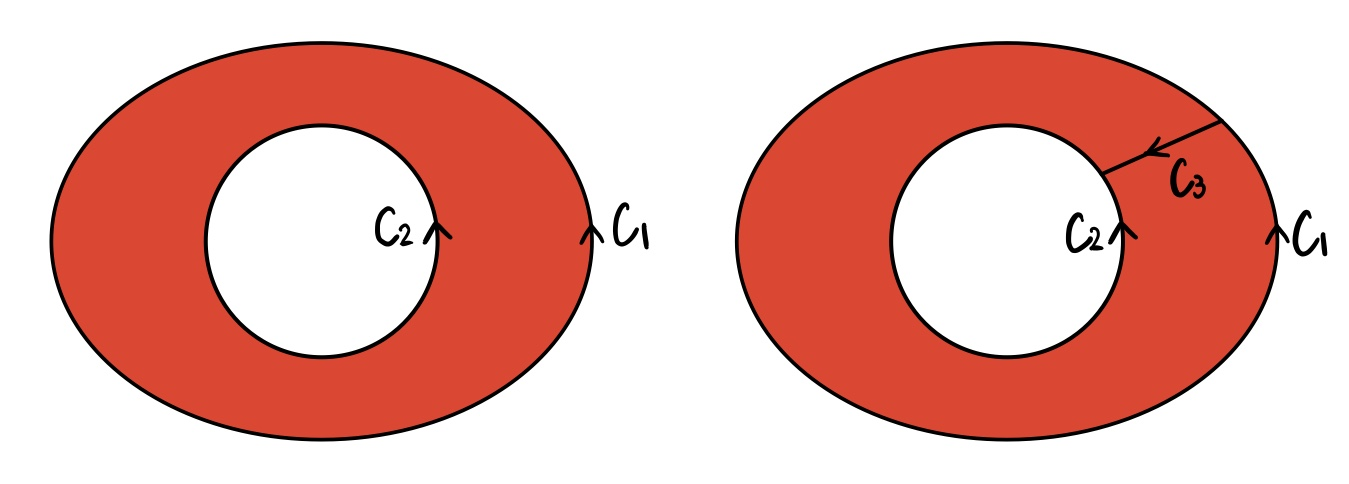
\includegraphics[scale=0.2]{19_1} 
\centering
\end{figure}
\\
Let $z \in \Omega$ and $C: C_1 \cup C_3 \cup -C_2 \cup -C_3$ be a closed curve about $z$ in $\Omega$. \\
Now Cauchy's Integral Formula applies
$$ f(z) = \frac{1}{2\pi i}\oint_C \frac{f(w)}{w - z} \, dw = \frac{1}{2\pi i}\oint_{C_1\cup -C_2} \frac{f(w)}{w - z} \,dw = \frac{1}{2\pi i} \oint_{C_1} \frac{f(w)}{w - z} \,dw - \frac{1}{2\pi i} \oint_{C_2} \frac{f(w)}{w - z} \,dw$$
\newline
\textbf{Laurent's Theorem.} \\
For $z \in A$ and $f$ holomorphic in 
$$A = \{z|r_1 < |z - z_0| < r_2\}$$
we have 
\begin{align*}
f(z) &= \sum_{n = -\infty}^{\infty} a_n(z - z_0)^n \\
a_n & = \frac{1}{2\pi i}\oint_C \frac{f(w)}{(w - z_0)^{n + 1}}\, dw
\end{align*}
where $C$ is any closed simple path in $A$ about $z_0$. \\
We may also use different notation for the coefficients with negative indices, $b_n = -a_n$. \\
\newline
\begin{minipage}{.5\textwidth}
       \begin{align*}
	f(z) &= \sum_{n = 1}^{\infty}\frac{b_n}{(z - z_0)^n} + \sum_{n = 0}^{\infty} a_n (z-z_0)^n \\
	a_n &= \frac{1}{2\pi i}\oint_C \frac{f(w)}{(w - z_0)^{n + 1}} \, dw \\
	b_n &= \frac{1}{2\pi i}\oint_C f(w)(w - z_0)^{n - 1} \, dw \\
	\end{align*}
  \end{minipage}%
  \begin{minipage}{.5\textwidth}
    \centering
    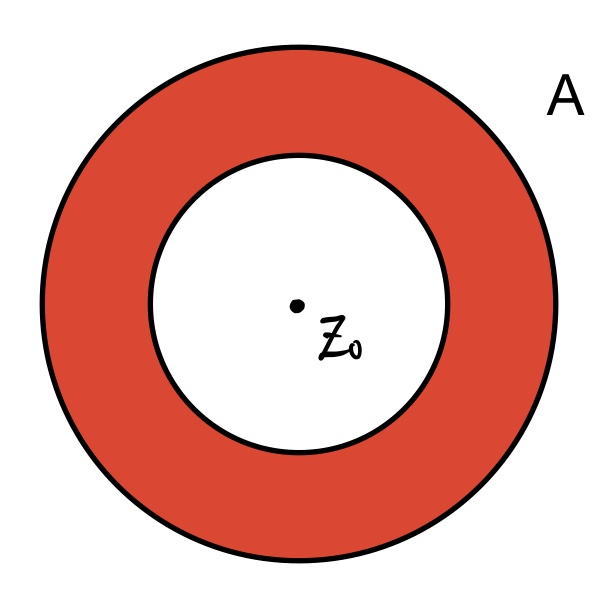
\includegraphics[scale = 0.2]{19_2}
\end{minipage} 
\newline
\newline
\textbf{Proof.}
Let $A = \{z|r_1 < |z - z_0| < r_2\}$ be an annulus centered at $z_0$. Choose $C_1$ and $C_2$, counter-clockwise circles in $A$ such that $z$ is in the region bounded by between them. We will assume $z_0 = 0$. By First Extension of Cauchy's Integral Formula,
$$f(z) = \frac{1}{2\pi i} \oint_{C_1} \frac{f(w)}{w - z} \,dw - \frac{1}{2\pi i} \oint_{C_2} \frac{f(w)}{w - z} \,dw$$
As shown earlier with Taylor Series: 
\begin{align*}
\frac{1}{2\pi i} \oint_{C_1} \frac{f(w)}{w - z} \,dw &= \sum_{n = 0}^{\infty} a_n z^n \\
a_n &= \frac{1}{2\pi i}\oint_{C_1} \frac{f(w)}{w^{n + 1}} \, dw
\end{align*}
provided $|z| < r_2$.
Then we transform the integral over $C_2$ as follows. 
$$\frac{1}{2\pi i}\oint_{C_2}\frac{f(w)}{w - z} \,dw = \frac{-1}{2\pi i}\oint_{C_2} \frac{f(w)}{z} \cdot \frac{1}{1 - \frac{w}{z}} \, dw = \frac{-1}{2\pi i}\oint_{C_2}\frac{f(w)}{z}\sum_{n = 0}^{\infty} \left(\frac{w}{z}\right)^n \, dw = \frac{-1}{2\pi i}\oint_{C_2}\sum_{n = 0}^{\infty} f(w)\frac{w^n}{z^{n + 1}} \, dw$$
Because the function $f(w)w^n$ is holomorphic in $A$ for all $n \in \mathbb{z}$, we can change the curve we are integrating over to $C_1$ or any other curve in $A$. Hence 
$$\frac{-1}{2\pi i}\oint_{C_2}\sum_{n = 0}^{\infty} f(w)\frac{w^n}{z^{n + 1}} \, dw = \frac{-1}{2\pi i}\oint_{C_1}\sum_{n = 0}^{\infty} f(w)\frac{w^n}{z^{n + 1}} \, dw $$
And since the Geometric Series converges uniformly for $\abs*{\frac{w}{z}} \leqslant r < 1$, we can swap the order of integration and summation.
$$\frac{-1}{2\pi i}\oint_{C_1}\sum_{n = 0}^{\infty} f(w)\frac{w^n}{z^{n + 1}} \, dw = \frac{-1}{2\pi i}\sum_{n = 0}^{\infty}\oint_{C_1} f(w)w^n \, dw \, \frac{1}{z^{n + 1}}$$
We rewrite $\frac{1}{z^{n + 1}}$ with $z^{-n - 1}$ and reindex our sum to start at $n = 1$. Therefore, 
\begin{align*}
\frac{1}{2\pi i}\oint_{-C_2}\frac{f(w)}{w - z} \,dw &= \sum_{n = 1}^{\infty} b_n z^{-n}, |z| > r \\
b_n &= \frac{1}{2\pi i}\oint_{C_1}f(w)w^{n - 1}\, dw 
\end{align*}
\newline
\textbf{Techniques.}
 We have two tricks to transform Power Series into forms we can manipulate. 
\begin{enumerate}
\item Treat $r = \frac{z}{w}$. If $|\frac{z}{w}| < 1$, $|z| < |w|$, the sum converges. 
$$\frac{1}{w - z} = \frac{1}{w}\cdot \frac{1}{1 - \frac{z}{w}} = \frac{1}{w}\left(1 + \frac{z}{w} + \left(\frac{z}{w}\right)^2+\cdots \right)$$
\item Treat $r = \frac{w}{z}$. If $|\frac{w}{z}| < 1$, $|w| < |z|$, the sum converges. 
$$\frac{1}{w - z} = \frac{-1}{z}\cdot \frac{1}{1 - \frac{w}{z}} = \frac{-1}{z}\left(1 + \frac{w}{z} + \left(\frac{w}{z}\right)^2+\cdots \right)$$
\end{enumerate}
\newpage
Laurent Series can be differentiated and integrated term by term to get $f'(z)$ or $F(z)$, since we have uniform convergence on closed annuli in $A$. We can understand Laurent Series as a "double-ended" Taylor Series. 
\begin{align*}
f(z) &= \cdots + \frac{a_{-2}}{z^2} + \frac{a_{-1}}{z} + a_0 + a_1z + a_2z^2 + \cdots \\ 
&= {\underbrace{\cdots + \frac{b_{2}}{z^2} + \frac{b_{1}}{z}}_\text{Singular/Principal Part}} + {\underbrace {a_0 + a_1z + a_2z^2 + \cdots}_\text{Regular/Analytic Part}}
\end{align*}
The structure of the principal part will tell us about $f$'s singularities at $z_0$. \\
We do not often find $a_n$'s from the formula, but follow the three rules. 
\begin{enumerate}
\item Break up $f(z)$ by Prime Factor Decomposition. 
\item Expand each term in $|z - z_0| < r$ or $|z - z_0| > R$. \\
The radius is often the distance to the next closest singularity of $f(z)$. 
\item Collect the needed terms from the step above for each element of the Prime Factor Decomposition. 
\end{enumerate} 

\textbf{Example.} Expand 
$$\frac{z}{z^2 + 1}, \, z_0 = i$$ 
There is a root of $z^2 + 1$ at $i$. 
$$\frac{z}{z^2 + 1} = \frac{1}{2}\cdot \frac{1}{z - i} + \frac{1}{2}\cdot \frac{1}{z + i}$$
The second term has a Taylor expansion at $z_0 = i$. 
$$\frac{1}{2}\cdot \frac{1}{z + i} = \frac{1}{2}\cdot \frac{1}{2i}\cdot \frac{1}{1-\left(-\frac{z-i}{2i}\right)} = \frac{1}{4i}\sum_{n = 0}^{\infty}(-1)^n\left(\frac{z - i}{2i}\right)^n $$
Therefore, we have the Laurent series of $\frac{z}{z^2 + 1}$ around $z_0 = i$ for $\abs*{\frac{z - i}{2i}} < 1$.
$$\Rightarrow \frac{z}{z^2 + 1} = {\underbrace{\frac{1}{2} \cdot \frac{1}{z - i}}_\text{Principal Part}} + {\underbrace{\frac{1}{4i}\sum_{n = 0}^{\infty}(-1)^n\left(\frac{z - i}{2i}\right)^n}_\text{Regular Part}}$$
\newline
\textbf{Example.} Expand 
$$ f(z) = \frac{1}{z + 1} + \frac{1}{z + 3}, \, z_0 = 0$$
In this case, we have three annuli. And we have two expressions for each simple partial fraction. 

\begin{align*}
\mbox{For } |z| < 1: \frac{1}{z + 1} &= \frac{1}{1 - (-z)} = \sum_{n = 0}^{\infty} (-1)^nz^n\\
\mbox{For } |z| > 1: \frac{1}{z + 1} &= \frac{1}{z} \cdot \frac{1}{1 - \left(\frac{-1}{z}\right)} = \frac{1}{z} \sum_{n = 0}^{\infty}\frac{(-1)^n}{z^n} = \sum_{n = 0}^{\infty}\frac{(-1)^n}{z^{n + 1}}\\ 
\mbox{For } |z| < 3: \frac{1}{z + 3} &= \frac{1}{3} \cdot \frac{1}{1 - \left(\frac{-z}{3}\right)} = \frac{1}{3} \sum_{n = 0}^{\infty}(-1)^n\left(\frac{z}{3}\right)^n \\
\mbox{For } |z| > 3: \frac{1}{z + 3} &= \frac{1}{z} \cdot \frac{1}{1 - \left(\frac{-3}{z}\right)} = \frac{1}{z} \sum_{n = 0}^{\infty}(-1)^n\left(\frac{3}{z}\right)^n = \sum_{n = 0}^{\infty}(-1)^n\frac{3^n}{z^{n + 1}}
\end{align*}
Therefore, 
\begin{align*}
\mbox{If } |z| < 1: f(z) &= \sum_{n = 0}^{\infty}(-1)^nz^n + \frac{1}{3} \sum_{n = 0}^{\infty}(-1)^n\left(\frac{z}{3}\right)^n \\
\mbox{It only has regular} &\mbox{ terms since } f \mbox{ is holomorphic on } |z| < 1. \\
\mbox{If } 1 < |z| < 3: f(z) &= \sum_{n = 0}^{\infty} \frac{(-1)^n}{z^{n + 1}} + \frac{1}{3}\sum_{n = 0}^{\infty}(-1)^n\left(\frac{z}{3}\right)^n\\
\mbox{If } |z| > 3: f(z) &= \sum_{n = 0}^{\infty}\frac{(-1)^n}{z^{n + 1}} + \sum_{n = 0}^{\infty}(-1)^n\frac{3^n}{z^{n + 1}} \\
\mbox{It only} &\mbox{ has singular terms}. \\
\end{align*}
\newline
\textbf{Example.} If 
$$f(z) = \frac{1}{\sin(z)}$$ 
has $\infty$-many singularities in $\mathbb{C}$, we will need expansions for $k\pi < |z| < (k+1)\pi, k \in \mathbb{N}$. 
\begin{figure}[h]
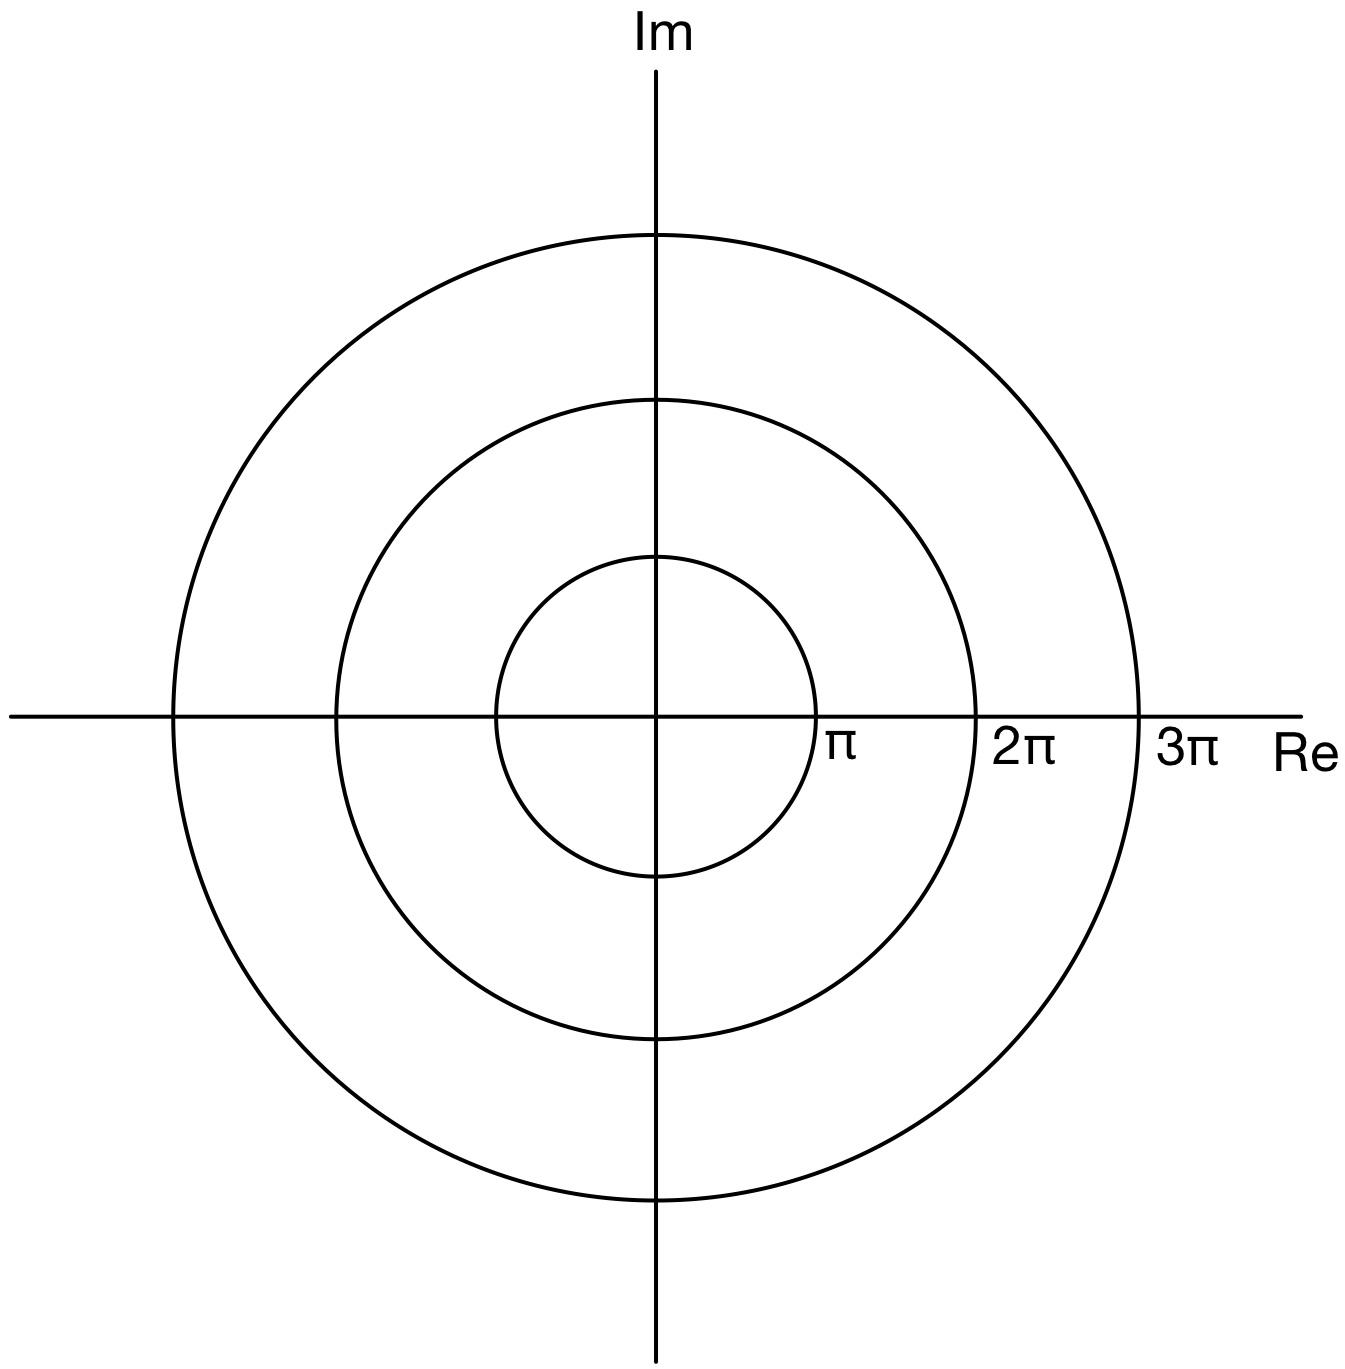
\includegraphics[scale=0.2]{19_3} 
\centering
\end{figure}
\\
\newpage
\section{Residue Theorem}
\subsection{Singularity and Root}
\textbf{Singularity.} \\
Let $f: \Omega \to \mathbb{C}$. Then $f$ has a singularity at $z_0$ if $f$ is not $\mathbb{C}$-differentiable at $z_0$. \\
\newline
\textbf{Isolated Singularity.} \\
If $f$ is holomorphic on the deleted or punctured disk $0 < |z - z_0| < \delta$ for some $\delta > 0$,  then the singularity is isolated. \\
\newline
\textbf{Example.} \\
$\operatorname{Log}(z)$ has a branch point at $z = 0$, every neighborhood of 0 intersects the branch cut of $\operatorname{Log}(z)$. Therefore, $\operatorname{Log}(z)$ has a non-isolated singularity at 0. \\
On the other hand, $\frac{1}{z}$ has an isolated singularity at 0. \\
\newline
There is a natural connection between an isolated singularity and a root of a holomorphic function. If $f$ is $\mathbb{C}$-differentiable at $z_0$ and its Taylor expansion is of the form 
$$f(z) = \sum_{k = n}^{\infty} a_k(z - z_0)^k = a_n(z-z_0)^n + a_{n + 1}(z - z_0)^{n + 1}+ \cdots$$
If $n = 1$, then $f$ has a simple root at $z_0$. \\
\newline
\textbf{Pole.} \\
We want to do the same thing for the principal/singular expansion for $f(z)$. For simplicity, let $b_n = a_{-n}$ to identify the singular coefficients. If 
$$f(z) = \sum_{k = -n}^{\infty} a_k(z - z_0)^k = \frac{b_n}{(z - z_0)^n} + \frac{b_{n - 1}}{(z - z_0)^{n - 1}} + \cdots$$
for $n > 0$ and $b_n \neq 0$, then $f$ has a pole of order $n$ at $z_0$. \\
If $b_n = 0$ for $n > 1$ and $|b_1| \neq 0$, then $f$ has a simple pole at $z_0$. \\
\newline
\textbf{Essential Singularity.} \\
If the principal part of $f(z)$ has $\infty$-many terms in it at $z_0$, then $f$ has an essential singularity or a non-removable pole at $z_0$. On the other hand, order-n poles are removable. \\
\newline
\textbf{Example.} $\sin(\frac{1}{x})$ has a non-removable pole at 0. \\
\newline
\textbf{Claim.} \\
If $f$ has an order $n$ root at $z_0$, $ f(z) \approx a_n(z - z_0)^n $ for $ z \approx z_0$. \\
If $f$ has an order $n$ pole at $z_0$, $f(z) \approx \frac{b_n}{(z - z_0)^n}$ for $z \approx z_0$. \\
\textbf{Proof.} Suppose $f$ has an order $n$ root at $z_0$. Since $a_n \neq 0$,
$$f(z) = \sum_{k = n}^{\infty}a_k(z - z_0)^k = a_n(z - z_0)^n\sum_{k = 0}^{\infty}\frac{a_k}{a_n}(z - z_0)^k$$
The proof with poles follows similarly. \\
We cannot correct for an essential singularity, but we can predict how the function will behave. \\
\newline
\textbf{Picard's Theorem.} \\
If $f$ has an essential singularity at $z_0$, then $f$ takes on all but possibly one value in $\mathbb{C}$ $\infty$-many times in any neighborhood near $z_0$. \\
\newline
\textbf{Meromorphic Function.} \\
A function is meromorphic on a domain $\Omega$ if $f$ is holomorphic on $\Omega$ except at isolated poles. Informally, these functions are the ratio of two holomorphic functions on $\Omega$. 
\\
\newline
On a bounded domain, a meromorphic function can only have finitely many isolated poles. Similar to the Uniqueness Theorem for holomorphic functions, zeros have to be isolated. \\
\newline
\textbf{Example.} \\
$\frac{1}{z}$ is meromorphic on $\mathbb{C}$. \\
$\csc(z)$ is meromorphic on $\mathbb{C}$, but it has $\infty$-many poles, namely $z = k\pi$ for $k \in \mathbb{Z}$. \\
\newline
\textbf{Example.} The meromorphic function 
$$ \frac{1}{1 - z} = \sum_{n = 0}^{\infty}z^n$$
has no singularity at $z = 0$, but does have a simple pole at $z = 1$. 
$$ \frac{1}{1 - z} = \frac{-1}{z - 1} + 0\cdot (z - 1)^0 + 0\cdot(z - 1)^1 + \cdots $$
Namely, the function is its singular part at $z = 1$. However, \\
$$ \frac{1}{1 - z} = \frac{-1}{z}\cdot \frac{1}{1 - \frac{1}{z}} = \sum_{n = 1}^{\infty} \frac{-1}{z^n}, \, |z| > 1$$
does have an essential singularity under a change of variables $w = \frac{1}{z}$. \\
Therefore, $\frac{1}{1-z}$ has an essential singularity at $\infty$. \\
\newline
For polynomial denominators, poles are easy to classify. \\
\textbf{Example.} 
$$ f(z) = \frac{z + 1}{z^3(z^2 + 1)}$$
has $\nth{3}$-order pole at $z = 0$ and $\nth{1}$-order poles at $z = \pm i$ \\
\newline
\textbf{Example.} 
$$ f(z) = \frac{\sin(z)}{z} = \frac{1}{z}\sum_{n = 0}^{\infty}\frac{z^{2n + 1}}{(2n)!} = 1 - \frac{z^2}{6} + \frac{z^4}{120} + \cdots$$
has no pole at $z = 0$, since $\sin(z)$ and $z$ have simple roots at 0. \\
Therefore, $f(z)$ has an isolated, removable singularity at 0.
\newpage
\subsection{Residue and Laurent Series}
\textbf{Residue.} \\
Suppose $f$ has an isolated singularity at $z_0$ and a Laurent Series on the annulus 
$$A = \{z\,|\, 0 < |z - z_0| < r\}$$
(The function has no other singularities in $A$.) \\
The residue of $f(z)$ at $z_0$ is given by 
$$Res(f, z_0) = b_1 = a_{-1}$$
\newline
Remember 
$$
\oint_C z^k \, dz = 
\begin{cases}
	0, \mbox{ if } k \neq -1 \\
	2\pi i \mbox{ if } k = -1
\end{cases}
$$
for any closed simple curve about 0. \\
\begin{figure}[h]
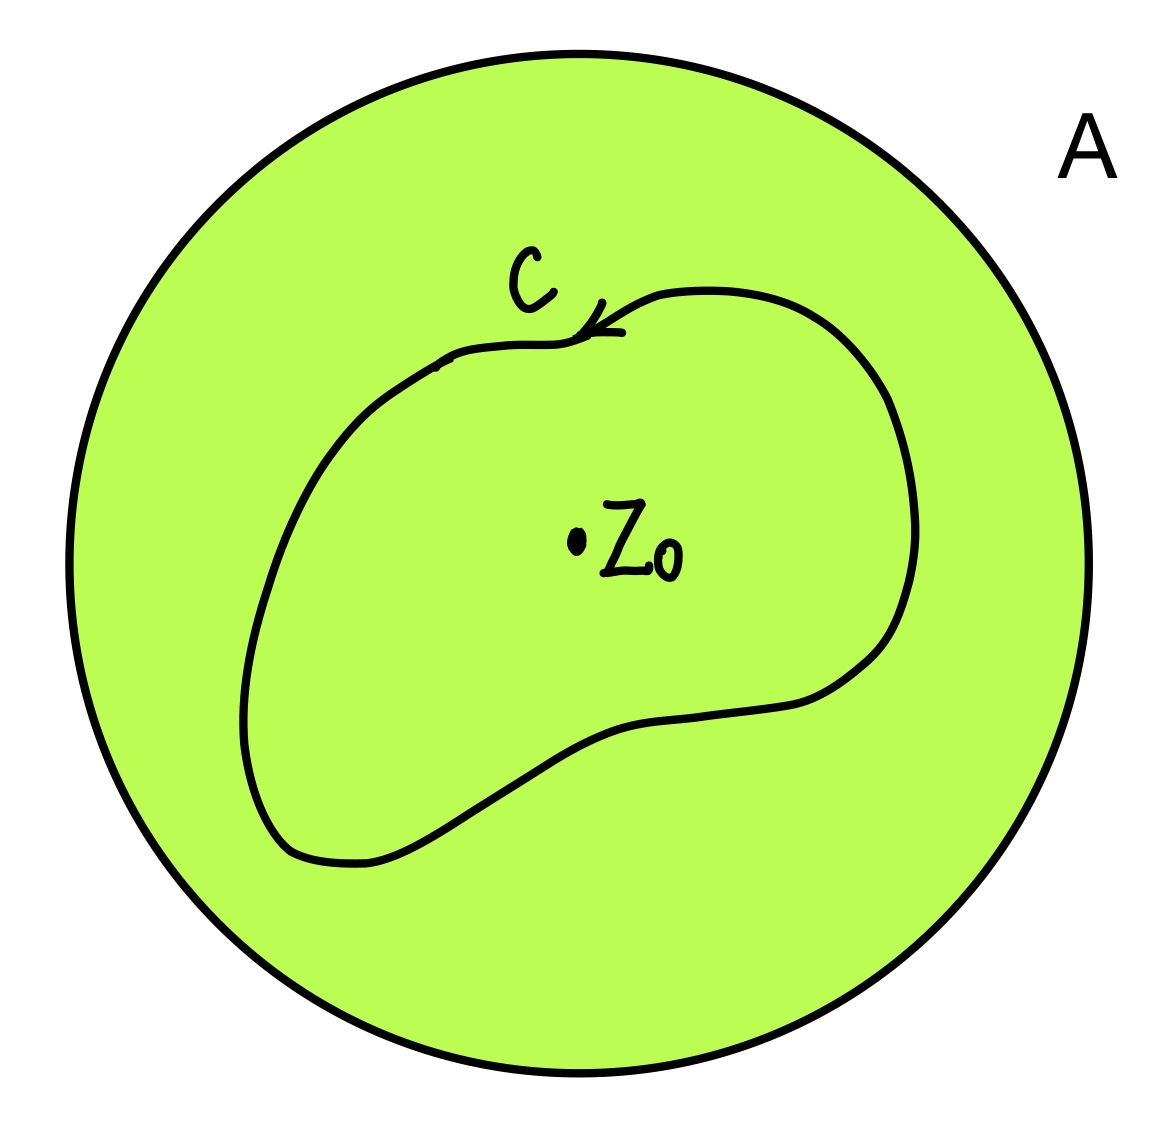
\includegraphics[scale=0.17]{20_1} 
\centering
\end{figure}
\\
For any closed simple counter-clockwise curve $C$ in $A$ about $z_0$, we have 
$$
\oint_C (z - z_0)^k \, dz = 
\begin{cases}
	0, \mbox{ if } k \neq -1 \\
	2\pi i \mbox{ if } k = -1
\end{cases}
$$
Therefore, 
$$ \oint_C f(z) \, dz = \oint_C \sum_{k = -n} ^ {\infty} a_k (z - z_0)^k \, dz = 2\pi i a_{-1} = 2\pi ib_1 = 2\pi i Res(f, z_0)$$
\newline
\textbf{Example.} If 
$$ f(z) = \frac{1}{z^3} + \frac{2}{z^2} + \frac{4}{z} + 5$$
then we have a pole of order 3 at 0 and $Res(f, 0) = 4$. \\
\newline
Not every Laurent expansion about a pole may be used to compute residues. \\
\newline
\textbf{Example.} Let 
$$ f(z) = \frac{-1}{z}\cdot \frac{1}{1-z} = -\frac{1}{z}\sum_{n = 0}^{\infty}z^n = -\frac{1}{z} - 1 - z - z^2 - \cdots$$
for $0 < |z| < 1$. Therefore, $f(z)$ has a simple pole and $Res(f, 0) = -1$. However, 
$$ f(z) = \frac{1}{z^2}\cdot \frac{1}{1 - \frac{1}{z}} = \frac{1}{z^2}\sum_{n = 0}^{\infty} \frac{1}{z^n} = \frac{1}{z^2} + \frac{1}{z^3} + \frac{1}{z^4} + \cdots$$
for $|z| > 1$. But $Res(f, 0) \neq 0$ because this Laurent Series is not valid in a punctured disk containing 0. Hence, we must use the first result. 
$$ Res\left(\frac{1}{z(z-1)}, 0\right) = -1$$
\newline
\textbf{Example.} $\operatorname{Log}(z)$ has a non-isolated singularity at 0. \\
Therefore, $Res(\operatorname{Log}(z), 0)$ does not exist. \\
\newline
\textbf{Empirical Rules.} 
\begin{enumerate}[leftmargin=*]
\item If 
$$ f(z) = \sum_{n = -1}^{\infty} a_n (z-z_0)^n $$
then 
$$Res(f(z), z_0) = a_{-1} = b_1$$
and $f$ has a simple pole at $z_0$.
\item If $ g(z) = (z - z_0)f(z) $ is $\mathbb{C}$-differentiable at $z_0$, then $ Res(f(z), z_0) = g(z_0)$.
\item If $f$ has a simple pole at $z_0$, then $$ \lim_{z \to z_0} (z-z_0)f(z) = Res(f(z), z_0)$$
(The limit exists and we have equality.) \\
Conversely, if $$ \lim_{z \to z_0} (z-z_0)f(z)$$ exists, then $f$ has a simple pole at $z_0$ or $f$ is $\mathbb{C}$-differentiable at $z_0$ and 
$$ \lim_{z \to z_0}(z - z_0)f(z) = Res(f(z), z_0)$$
\item If $f$ has a simple pole at $z_0$ and $g(z)$ is $\mathbb{C}$-differentiable at $z_0$, 
$$ Res(fg, z_0) = g(z_0)\,Res(f, z_0)$$
If $g(z_0) \neq 0$, 
$$ Res\left(\frac{f}{g}, z_0\right) = \frac{Res(f, z_0)}{g(z_0)} $$
\item If $g$ has a simple root at $z_0$, then $\frac{1}{g}$ has a simple pole at $z_0$ and 
$$ Res\left(\frac{1}{g}, z_0\right) = \frac{1}{g'(z_0)} $$
\item If $f$ has a pole of order $k$ at $z_0$, then $g(z) = (z - z_0)^kf(z)$ is holomorphic and for 
$$g(z) = a_0 + a_1(z - z_0) + \cdots$$
we have 
$$ Res(f, z_0) = a_{k - 1} = \frac{g^{k - 1}(z_0)}{(k - 1)!}$$
\end{enumerate}
Each of these can be shown by studying $f$'s Laurent expansion in $ 0 < |z - z_0| < \delta$. \\
\newline
\textbf{Example.} 
$$f(z) = \frac{z^2 + z + 2}{(z - 2)(z - 3)(z - 4)(z - 5)}$$ 
at $z = 2$ we have a simple pole and $g(z) = (z - 2)f(z)$ is holomorphic. \\
Therefore by \circled{\scriptsize3} $Res(f, 2) = g(2) = -\frac{4}{3}$. \\
We do not need to compute the Laurent Series at $z_0 = 2$. \\
\newline
\textbf{Example.}
$$ f(z) = \frac{1}{\sin(z)}$$ 
Then by \circled{\scriptsize5} 
$$Res(f(z), \pi k) = \frac{1}{\cos(\pi k)} = (-1)^k $$
\newline
\textbf{Example.} Since 
$$\sinh(z) = z + \frac{z^3}{3!} + \frac{z^5}{5!} + \cdots = \sum_{n = 0}^{\infty}\frac{z^{2n + 1}}{(2n + 1)!}$$
Then 
$$ f(z) = \frac{\sinh(z)}{z^5} = \frac{1}{z^4} + \frac{1}{6z^2} + \frac{1}{120} + \cdots $$
Therefore, $Res(f, 0) = 0$. \\
\newline
\textbf{Example.}
$$ f(z) = \frac{1}{z(z - 2)^2}, \, g(z) = (z - 2)^2f(z) = \frac{1}{z}$$
Then by \circled{\scriptsize 6} 
$$ Res(f, 2) = g'(2) = \frac{-1}{z^2} \bigg\rvert_{z = 2} = -\frac{1}{4}$$ 
\newline
\textbf{Example.} 
$$ f(z) = \frac{1}{z(z - 2)^3}, \, g(z) = (z - 2)^3f(z) = \frac{1}{z}$$
Then by \circled{\scriptsize 6} 
$$ Res(f, 2) = \frac{g''(2)}{2} = \frac{1}{z^3} \bigg\rvert_{z = 2} = \frac{1}{8}$$ 
\newpage
\textbf{Example.} 
$$\cot(z) = \frac{\cos(t)}{\sin(t)} = \frac{b_1}{z} + a_0 + a_1z + a_2z^2 + \cdots = \frac{1 - \frac{z^2}{2} + \frac{z^4}{4!} - \cdots}{z - \frac{z^3}{6} + \frac{z^5}{5!} - \cdots}$$
We have a system of equations
$$(\frac{b_1}{z} + a_0 + a_1z + a_2z^2 + \cdots)(z - \frac{z^3}{6} + \frac{z^5}{5!} - \cdots) = 1 - \frac{z^2}{2} + \frac{z^4}{4!} - \cdots$$
After we equate the powers of $z$, we have
$$b_1 + a_0z + (-\frac{b_1}{6} + a_1)z^2 + (-\frac{a_0}{6} + a_2)z^3 + (\frac{b_1}{5} - \frac{a_1}{6} + a_3)z^4 = 1 - \frac{z^2}{2} + \frac{z^4}{4!}$$
Therefore, $a_0 = 0, a_1 = -\frac{1}{3}, a_2 = 0, a_3 = -\frac{1}{45}, b_1 = 1$. This means 
$$\cot(z) = \frac{1}{z} - \frac{z}{3} - \frac{z^3}{45} + \cdots $$
\newline
\textbf{Cauchy's Residue Theorem.} \\
Let $\Omega$ be a domain in $\mathbb{C}$ and $f$ is holomorphic on $\Omega$ except at finitely many isolated singularities. Then for any simple-closed curve $C$ in $\Omega$ that does not pass through any singularity of $f$, oriented counter-clockwise, we have
$$ \oint_C f(z) \, dz = 2\pi i \sum \mbox{residues of } f \mbox{ in } C$$
\textbf{Proof.} Assume $f$ has 2 singularities. This proof extends easily to finitely many. Consider a path around $f$'s singularities, $z_1$ and $z_2$.
\begin{figure}[h]
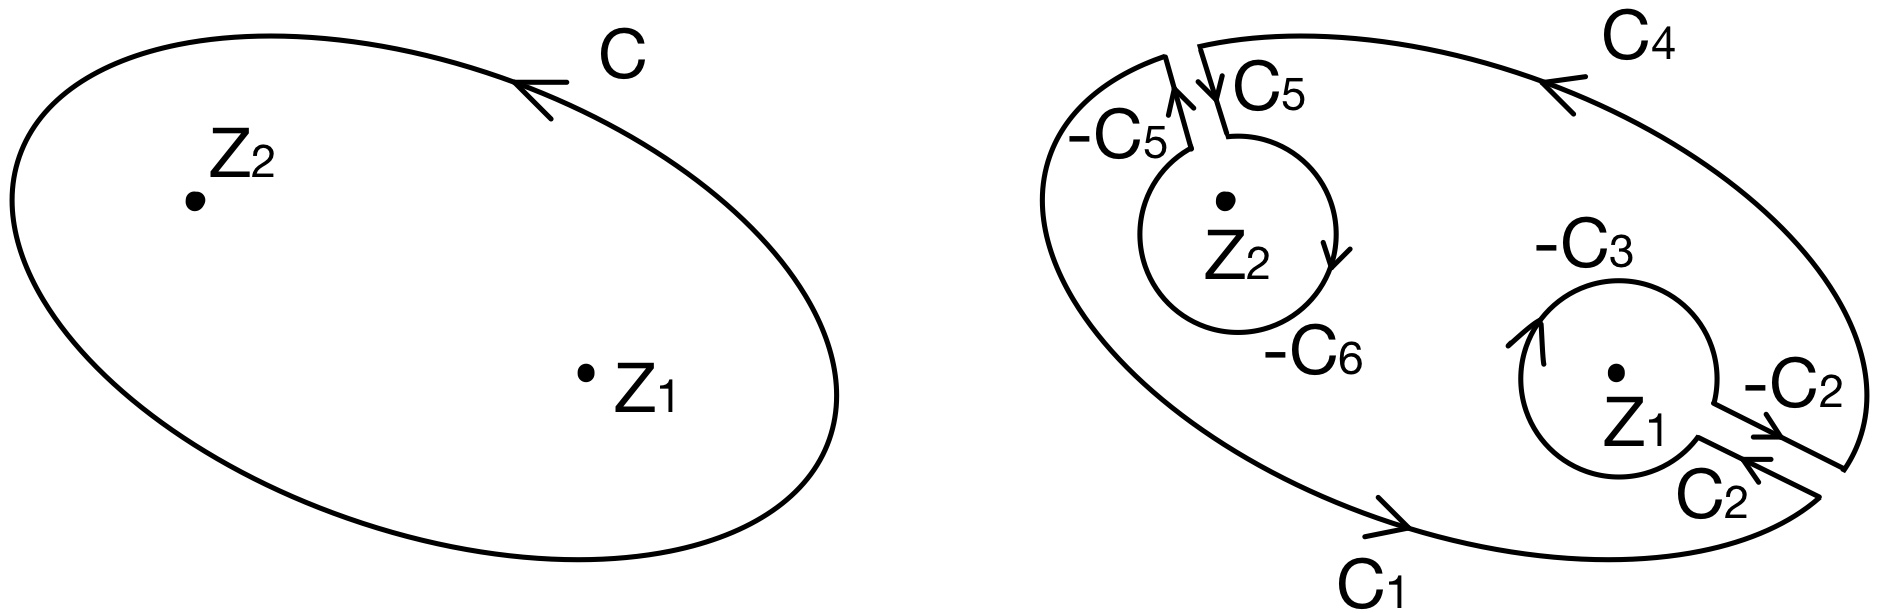
\includegraphics[scale=0.2]{20_2} 
\centering
\end{figure}
\begin{align*}
C_0 &= C_1 \cup C_2 \cup -C_3 \cup -C_2 \cup C_4 \cup C_5 \cup -C_6 \cup -C_5 \\
C &= C_1 \cup C_4
\end{align*}
By Cauchy-Goursat Theorem, 
$$ \oint_{C_0}f(z) \, dz = 0$$
And the integrals over $\pm C_2$ and $\pm C_5$ sum to zero. Therefore, 
\begin{align*}
0 &= \oint_{C_0}f(z) \, dz = \oint_{C_1 \cup -C_3 \cup C_4 \cup -C_6} f(z) \, dz = \oint_{C_1 \cup C_4}f(z) \,dz + \oint_{-C_3 \cup -C_6} f(z) \,dz\\
\Rightarrow \oint_Cf(z) \, dz &= \oint_{C_3 \cup C_6} f(z) \, dz = \oint_{C_3}f(z) \,dz + \oint_{C_6}f(z)\,dz = 2\pi i(Res(f, z_1) + Res(f, z_2)) 
\end{align*}
Hence, this concludes the proof. 
\newpage
\textbf{Example.} 
$$f(z) = \frac{1}{z(z^2 + 1)} $$
\begin{figure}[h]
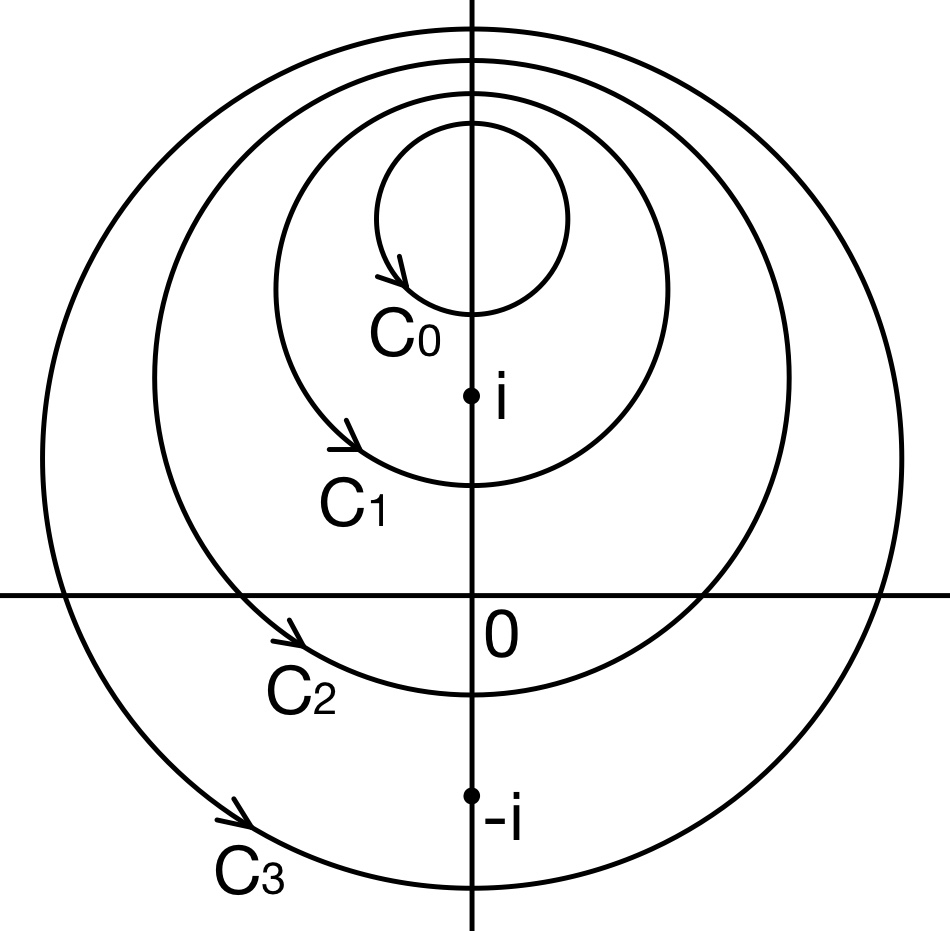
\includegraphics[scale=0.3]{20_3} 
\centering
\end{figure}
Then we can derive the following residues. 
\begin{align*}
Res(f, i) &= (z - i)f(z) \bigg\rvert_{z = i} = \frac{1}{i(i + 1)} = -\frac{1}{2}\\
Res(f, 0) &= zf(z) \bigg\rvert_{z = 0} = \frac{1}{0 + 1} = 1 \\
Res(f, -i) &= (z + i)f(z) \bigg\rvert_{z = -i} = \frac{1}{-i(-i - 1)} = -\frac{1}{2}
\end{align*}
When we traverse through the contours illustrated in the graph, we have 
\begin{align*}
\oint_{C_0}f(z)\,dz &= 0 \, \mbox{ by Cauchy-Goursat Theorem}\\
\oint_{C_1}f(z)\,dz &= 2\pi i \,Res(f,i) = -\pi i\\
\oint_{C_2}f(z)\,dz &= 2\pi i\left(Res(f, i) + Res(f, 0)\right) = -\pi i + 2\pi i = \pi i\\
\oint_{C_3}f(z)\,dz &= 2\pi i\left(Res(f, i) + Res(f, 0) + Res(f, -i)\right) =  -\pi i + 2\pi i - \pi i = 0
\end{align*}
But $f$ is not holomorphic on the interior of $C_3$. \\
\newpage
\textbf{Example.} Integrate
$$f(z) = \frac{1}{z(z - 2)^4}$$
over $|z - 2| = \frac{1}{3}$. Therefore, we need $Res(f, 2)$.
\begin{align*}
\frac{1}{z} &= \frac{1}{2 + (z - 2)} = \frac{1}{2} \cdot \frac{1}{1 - (-\frac{z - 2}{2})} = \frac{1}{2}\left(1 - \frac{z - 2}{2} + \frac{(z - 2)^2}{4} - \frac{(z - 2)^3}{8} + \cdots\right) \\
f(z) &= \frac{1}{2(z - 2)^4} - \frac{1}{4(z - 2)^3} + \frac{1}{8(z - 2)^2} - \frac{1}{16(z - 2)} + \cdots 
\end{align*}
Therefore, $Res(f, 2) = -\frac{1}{16}$. Hence, 
$$\oint_{|z - 2| = \frac{1}{3}}f(z) \, dz = 2\pi i \, Res(f, 2) = -\frac{\pi i}{8} $$

\newpage
\section{Improper Integrals}
\subsection{Principal Value}
Suppose 
$$ I = \int_{\mathbb{R}}f(x) \,dx$$
converges absolutely. Then
$$ I = \lim_{R\to\infty}\int_{-R}^{R}f(x) \, dx = P.V.\int_{\mathbb{R}}f(x) \, dx$$
Here 
$$ P.V.\int_{\mathbb{R}}f(x) \, dx = \lim_{R\to\infty}\int_{-R}^{R}f(x) \, dx $$ 
denotes the principal value of 
$$ \int_{\mathbb{R}}f(x)\, dx$$
However, without absolute convergence of $I$, this does not hold. \\
\newline
\textbf{Example.}
$$ \lim_{R \to \infty} \int_{-R} ^{R} \sin(x) \,dx = 0$$
but 
\begin{align*}
& \int_{\mathbb{R}}\sin(x) \, dx \text{ does not exist} \\
& \int_{\mathbb{R}}|\sin(x)| \,dx = \infty
\end{align*}
If $f(x)$ is undefined at $c \in (a, b)$, then 
$$ P.V. \int_b^a f(x) \, dx = \lim_{\varepsilon \to 0^+}\left(\int_{a}^{c - \varepsilon}f(x) \, dx + \int_{c + \varepsilon}^b f(x) \right)$$
\begin{figure}[h]
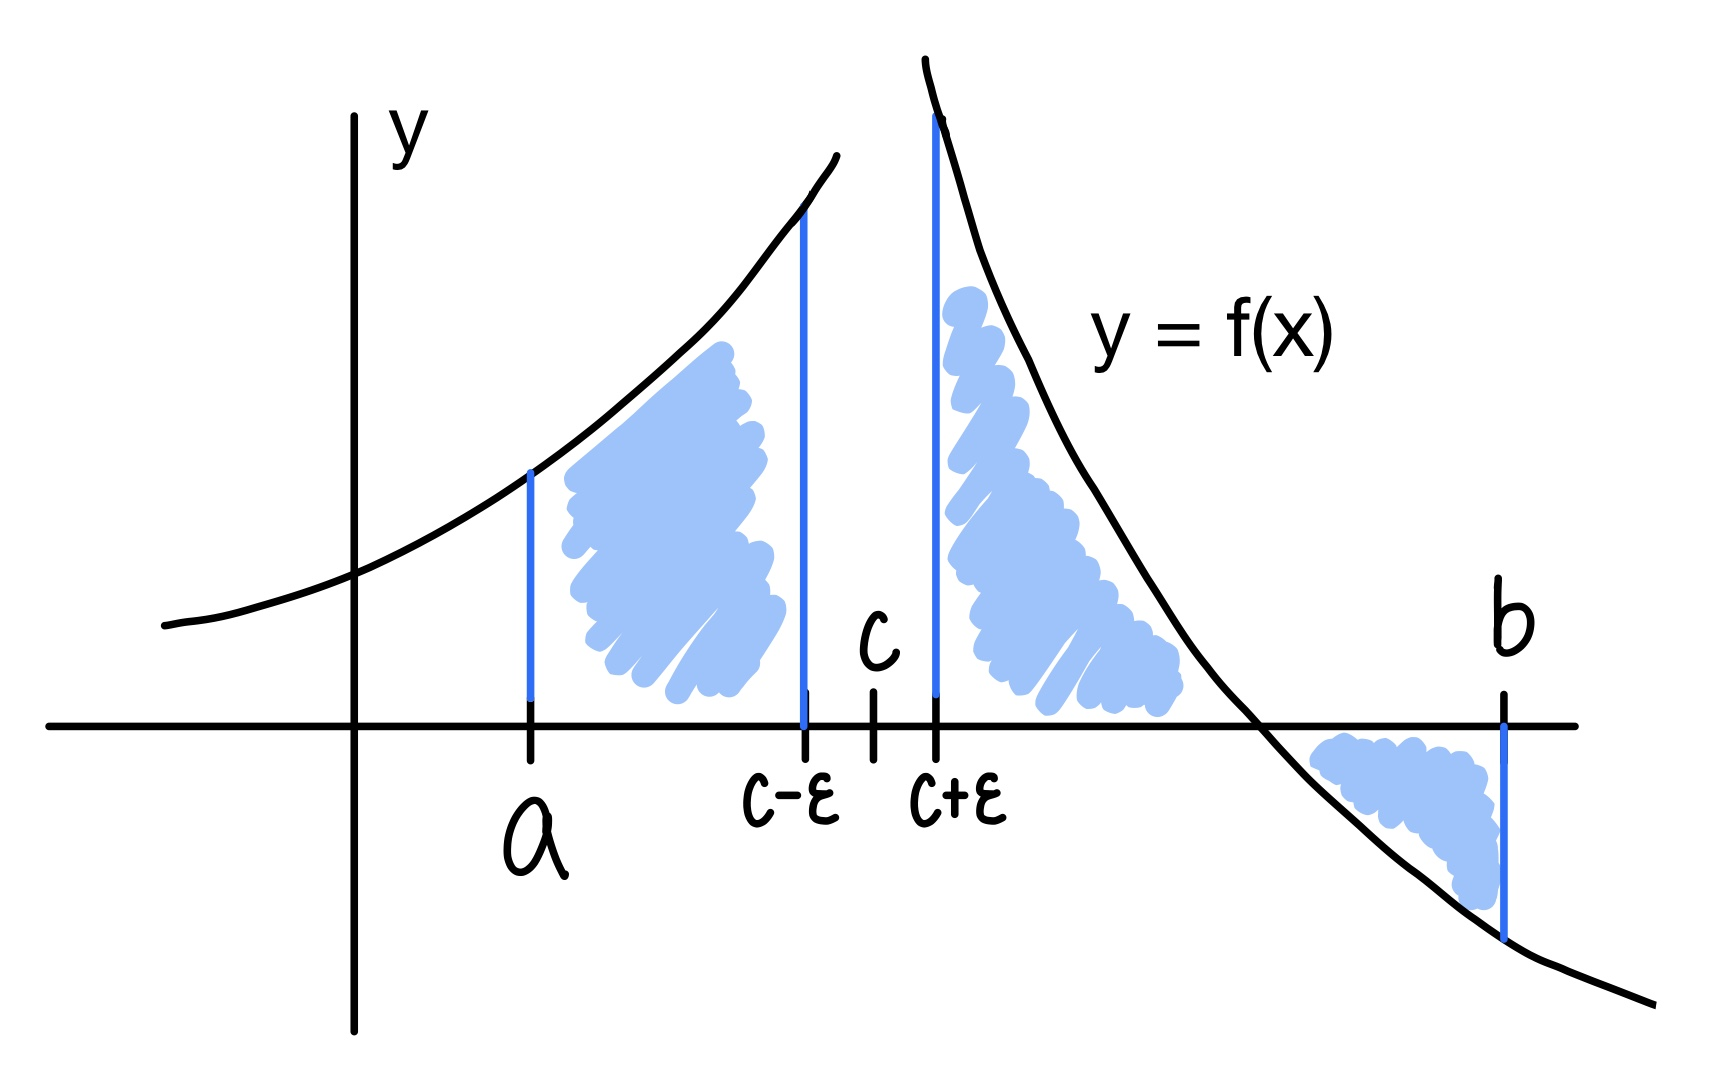
\includegraphics[scale=0.17]{21_1} 
\centering
\end{figure}
\newpage
\textbf{Example.} Let 
$$ f(x) = \frac{1}{x^3}$$
then 
\begin{align*}
I &= P.V.\int_{-2}^{3}f(x) \, dx \\
& = \lim_{\varepsilon \to 0^+} {\int_{-2}^{-\varepsilon} f(x)\, dx + \int_{\varepsilon}^3 f(x) \, dx} \\
& = \lim_{\varepsilon \to 0^+} {F(3) - F(\varepsilon) + F(-\varepsilon) - F(-2)} \\
& = \lim_{\varepsilon \to 0^+} {F(3) - F(-2)} \\
& = \frac{-1}{2x^2} \bigg\rvert_{x = -2}^{3}
\end{align*}
since $F$ is even. We are "ignoring" the singularity by exploiting 
$$ \int_{-a}^{a}f(x) \, dx = 0$$
for $f$ odd and piecewise-smooth. \\
\newline
\textbf{Lemma.} \\
If $|f(x)| \leqslant g(x)$ for all $x \in \mathbb{R}$ and $\int_{\mathbb{R}}g(x) \, dx$ converges, then 
$$ I = \int_{\mathbb{R}} f(x) \, dx$$ 
converges absolutely. 
\subsection{Clever Choice of Contours.}
\textbf{$\text{Example}^\star$.} The improper integral 
$$ \int_{\mathbb{R}}\frac{1}{(x^2 + 1)^2} \, dx$$
converges absolutely because 
$$ \frac{1}{(x^2 + 1)^2} \leqslant \frac{1}{(x^2 + 1)} \text{ and } \int_{\mathbb{R}}\frac{1}{(x^2 + 1)} \, dx < \infty$$
Let 
$$ f(z) = \frac{1}{(z^2 + 1)^2} = \frac{1}{(z + i)^2(z - i)^2} $$
and by Residue Theorem, 
$$ \oint_C f(z) \,dz = 2\pi i\, Res(f, i)$$
for any closed curve $C$ about $i$, but not $-i$. \\
\begin{figure}
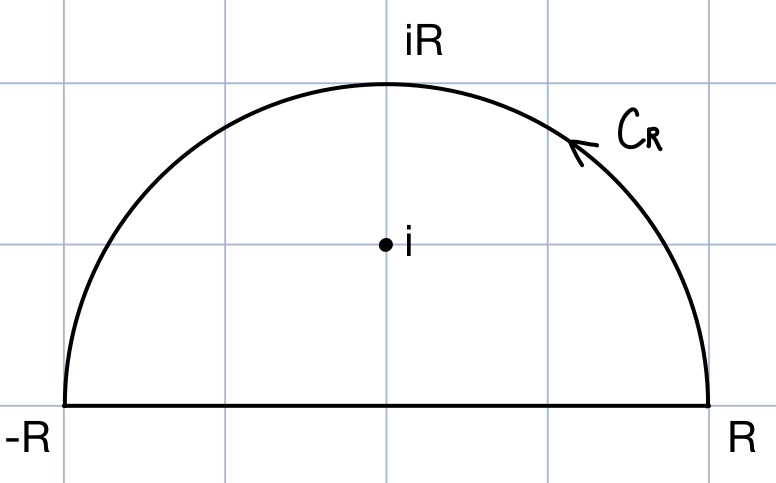
\includegraphics[scale=0.2]{21_2} 
\centering
\end{figure}
\newline
\newpage
We pick a path along $[-R, R]$ and the upper half of the disk $|z| = R$ traversed counter-clockwise. Therefore,
$$2\pi i \, Res(f, i) = \int_{C_R}f(z) \, dz + \oint_{-R}^{R}f(z) \, dz$$
then 
$$ \int_{\mathbb{R}} f(x) \, dx = \lim_{R \to \infty} \oint_C f(z) \, dz = \lim_{R \to \infty} \int_{-R}^{R} f(z) \, dz$$
provided
$$\lim_{R \to \infty} \int_{C_R} f(z) \, dz = 0$$
That is to say, the integral over the upper curve vanishes. We can establish this with an ML-Estimate, 
\begin{align*}
\abs{f(z)} &\leqslant \frac{A}{|z|^4} \text{ for z-large}, \,A > 0 \\
\Rightarrow \abs*{\int_{C_R}f(z) \, dz} &\leqslant \int_{C_R}|f(z)||dz| \leqslant {\underbrace{\frac{A}{R^4}}_{M}}{\underbrace{\pi R}_{L}} = \frac{A\pi}{R^3}
\end{align*}
Therefore, its upper bound $\to 0$ as $R \to \infty$. Therefore, 
$$\lim_{R \to \infty} \int_{C_R} f(z) \, dz = 0$$ 
Next we solve $Res(f, i)$. 
\begin{align*}
g(z) &= (z - i)^2f(z) = \frac{1}{(z + 2)^2} \\ 
Res(f, i) &= g'(i) = \frac{d}{dz}\frac{1}{(z + i)^2}\bigg\rvert_{z = i} = \frac{-2}{(z + i)^3}\bigg\rvert_{z = i} = \frac{1}{4i}
\end{align*}
Hence, 
$$ \int_{\mathbb{R}}f(x) \, dx = 2\pi i \, Res(f, i) = 2\pi i \cdot \frac{1}{4i} = \frac{\pi}{2}$$
This technique works whenever $|f(z)| \leqslant \frac{A}{|z|^a}, a > 1$ and $z$-large.
\newpage
\textbf{Example (Trigonometry).} Find 
$$ I = \int_{\mathbb{R}}\frac{\cos(x)}{(x - 1)^2 + 1} \, dx$$
$$ |I| = \int_{\mathbb{R}}\abs*{\frac{\cos(x)}{(x - 1)^2 + 1}} \, dx \leqslant \int_{\mathbb{R}}\frac{A}{x^2 + 1} \, dx < \infty$$
Therefore, $I$ converges absolutely. Here $\cos(z) \to \infty$ as $z \to \infty$. \\
Replace $\cos(x)$ with $e^{ix} = \cos(x) + i\sin(x)$. 
$$ I^\ast = \int_{\mathbb{R}}\frac{e^{ix}}{(x - 1)^2 + 1} \, dx, \, I = \Re(I^\ast)$$
$$ f(z) = \frac{e^{iz}}{(z - 1)^2 + 1}, \, |f(z)| = \frac{|e^{i(x + iy)}|}{|z^2 - 2z + 2|} = \frac{e^{-y}}{|z^2 - 2z + 2|}$$
We evaluate the integral over the same contour, $C = C_R \cup [-R, R]$. With $y > 0$, for $z$-large we have 
$$\frac{e^{-y}}{|z^2 - 2z + 2|} \leqslant \frac{A}{|z|^2} $$
Repeating the argument from the previous example, we have 
$$ \lim_{R \to \infty} \int_{C_R}f(z) \,dz = 0$$
We have two poles, $z = 1 \pm i$ and only one is inside the curve $C$, $z = 1 + i$.
\begin{figure}[h]
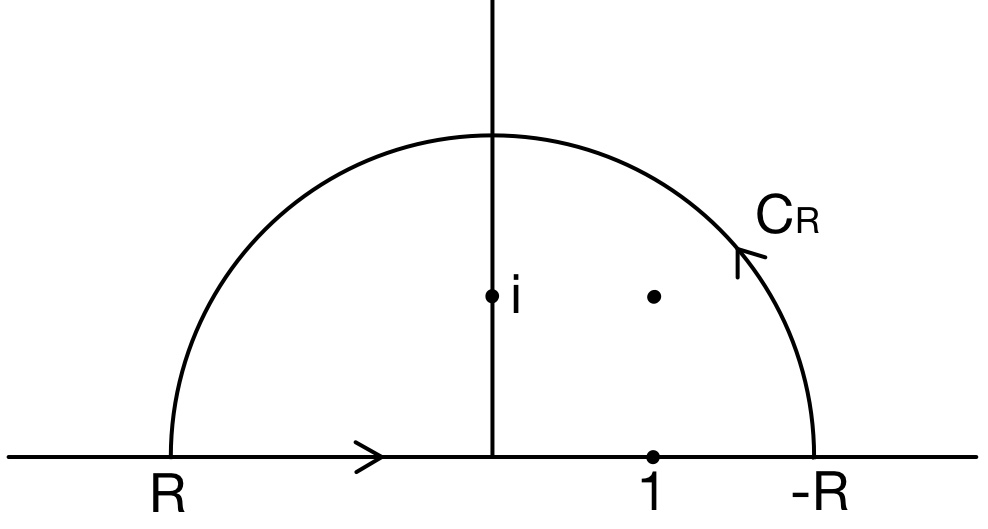
\includegraphics[scale=0.2]{21_3} 
\centering
\end{figure} 
\begin{align*}
I^\ast &= 2\pi i\,Res(f, 1 + i) = 2\pi i \left(-\frac{i}{2}e^{i - 1}\right) = \frac{\pi e^i}{e} \\
Res(f, 3i) &= \frac{e^{iz}}{z - (1 - i)}\bigg\rvert_{z = 1 + i} = -\frac{i}{2}e^{i - 1} \\
I &= \Re(I^\ast) = \Re\left(\pi \frac{e^i}{e}\right) = \frac{\pi}{e}\cos(1)
\end{align*}
\newpage
\textbf{Note.} The approach we used above $I = \Re(I ^\ast)$ fails for 
$$ I = \int_{\mathbb{R}}\frac{\cos(x)}{(x - 1)^3} \,dx$$
because $I \neq \conj{I}$ or $| \in \mathbb{C} \backslash \mathbb{R}$. \\
\textbf{Proof.} 
$$ I = \int_{\mathbb{R}}\frac{\cos(x)}{(x - i)^3} \,dx = \int_{\mathbb{R}}\frac{\cos(x)}{(x^2 + i)^3}(x + i)^3 \,dx = \int_{\mathbb{R}}\frac{\cos(x)}{(x^2 + i)^3}(x^3 + 3ix^2 - 3x - i) \,dx $$
Let $f(x) = \frac{\cos(x)}{(x^2 + 1)^3}$, it is an even function. Thus, 
\begin{align*}
I &= \int_{\mathbb{R}}f(x) (x^3 + 3ix^2 - 3x - i) \, dx \\
&= \int_{\mathbb{R}}f(x)x^3 \,dx + \int_{\mathbb{R}}f(x)3ix^2 \,dx - \int_{\mathbb{R}}f(x)3x\,dx -  \int_{\mathbb{R}}if(x)\,dx \\
&= \int_{\mathbb{R}}f(x) 3ix^2 \,dx - \int_{\mathbb{R}}if(x)\,dx 
\end{align*}
The equality holds because 
$$ \int_{\mathbb{R}}f(x)x^3 \, dx = \int_{\mathbb{R}}f(x)3x \, dx = 0$$ 
as $f(x)x^3$ and $f(x)3x$ are both odd functions. Similarly, 
\begin{align*}
\conj{I} &= \int_{\mathbb{R}}\frac{\cos(x)}{(x + i)^3} \,dx \\
&= \int_{\mathbb{R}}\frac{\cos(x)}{(x^2 + i)^3}(x - i)^3 \,dx \\
&= \int_{\mathbb{R}}\frac{\cos(x)}{(x^2 + i)^3}(x^3 - 3ix^2 - 3x + i) \,dx \\
&= -\int_{\mathbb{R}}f(x) 3ix^2 \,dx + \int_{\mathbb{R}}if(x)\,dx
\end{align*}
Therefore, $I = \conj{I}$, which obviously does not satisfy $I = \conj{I}$. \\
\newline
\textbf{Example (Change of Variable). }\\
For 
$$ \int_0^{2\pi}g(\theta) \, d\theta$$ 
Let $z = e^{i\theta} \Rightarrow dz = ie^{i\theta}d\theta \Rightarrow d\theta = \frac{dz}{iz}$. Then 
$$ \int_0^{2\pi} \frac{d\theta}{5 + 2\cos\theta} = \oint_{|z| = 1}\frac{1}{iz}\cdot\frac{dz}{5 + z + \frac{1}{z}}$$ 
$$\text{for } \cos\theta = \frac{z + z^{-1}}{2}$$ 
Here the poles of the integrand are 
\begin{align*}
&z = \frac{-5 \pm \sqrt{21}}{2}, \abs*{\frac{-5 + \sqrt{21}}{2}} < 1 \text{ and } \abs*{\frac{-5 - \sqrt{21}}{2}} > 1 \\
\Rightarrow &\frac{1}{i} \oint_{|z| = 1} \frac{dz}{z^2 + 5z + 1} = \frac{2\pi i}{i} \frac{1}{(z - \frac{1}{2}(-5 - \sqrt{21}))} \Bigg\rvert_{z = \frac{-5 + \sqrt{21}}{2}} = \frac{2\pi}{\sqrt{21}}
\end{align*}
\newline
\textbf{Semicircle Lemma.} \\
Let $f(z)$ have a simple pole at $z_0$ and let $C_\varepsilon$ be the curve parametrized by 
$$ \gamma(t) = z_0 + \varepsilon e^{it}, t \in [0, \pi]$$
Then 
$$ \lim_{\varepsilon \to 0^+} \int_{C_\varepsilon}f(z) \, dz = \pi i \, Res(f, z_0)$$
\begin{figure}[h]
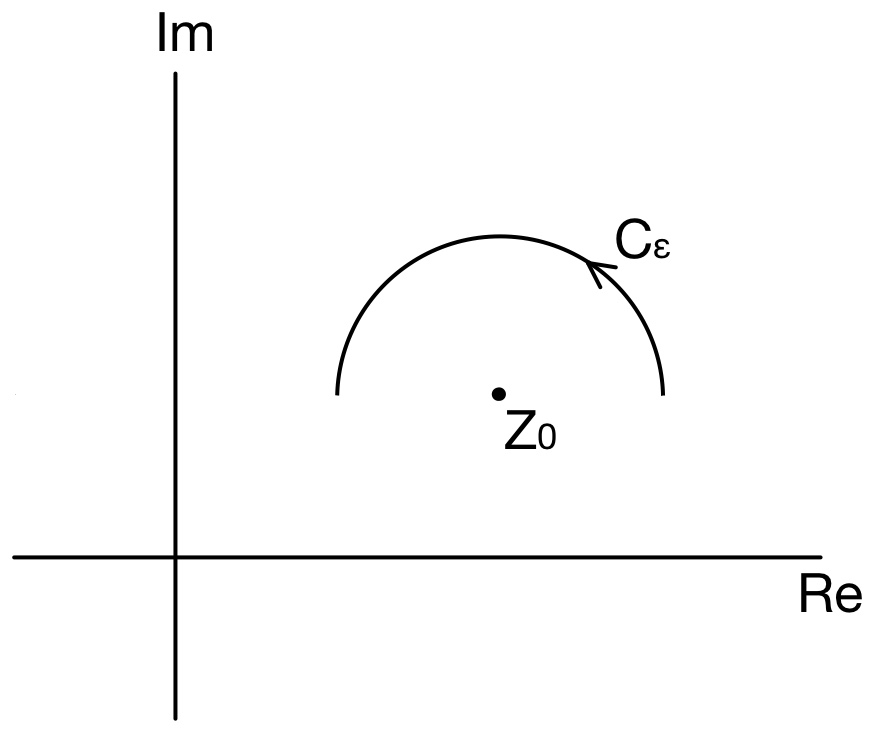
\includegraphics[scale=0.17]{21_4} 
\centering
\end{figure} 
\newline
\textbf{Proof.} Assume $\varepsilon > 0$ but small enough for $f$ to have a Laurent expansion for $0 < |z - z_0| < \varepsilon$. Then 
\begin{align*}
f(z) &= \frac{b_1}{z - z_0} + a_0 + a_1(z - z_0)+ \cdots \\
\int_Cf(z)\,dz &= \int_0^\pi f(z_0 + \varepsilon e^{it})\varepsilon i e^{it }dt \\ 
&= \int_0^\pi b_1i + a_0i\varepsilon e^{it} + a_1i\varepsilon^2e^{2it}+ \cdots dt
\end{align*}
and 
$$\lim_{\varepsilon \to 0^+}\int_C{f(z)}\, dz = \pi i b_1 = \pi i Res(f, z_0)$$
For non-simpe poles, the limit does not exist and we can extend this argument to any angular range.
\newpage
\textbf{Corollary of Semicircle Lemma.} \\
$$\lim_{\varepsilon \to 0^+} \int_{C_\varepsilon}f(z) \, dz = \theta i \, Res(f, z_0)$$
where $C_\epsilon$ is the curve parametrized by 
$$ \gamma(t) = z_0 + \varepsilon e^{it}, t \in [\alpha, \alpha + \theta] $$ 
\newline
\textbf{Jordan's Lemma.}\\
If for $z$-large, 
$ |f(z)| \leqslant \frac{A}{|z|} $ and $C_R$ is the curve parametrized by 
$$ \gamma(t) = Re^{it}, t \in [0, \pi]$$
then for $\alpha > 0$, 
$$ \lim_{R \to \infty}\int_{C_R}f(z) e^{i\alpha z}\, dz = 0$$ 
\newline
\newline
\textbf{Example.} Find 
$$ I = P.V.\int_{\mathbb{R}}\frac{e^{ix}}{x} \,dx$$
This integrand is not continuous at $x = 0$, 
$$ I = \lim_{R \to \infty, \varepsilon \to 0+} \int_{-R}^{\varepsilon}f(x) \, dx + \int_{\varepsilon}^{R}f(x) \, dx$$
We approach $x = 0$ from the left and right at the same rate and distance. \\
Let $f(z) = \frac{e^{iz}}{z}$ and consider the contour $C$.
\begin{figure}[h]
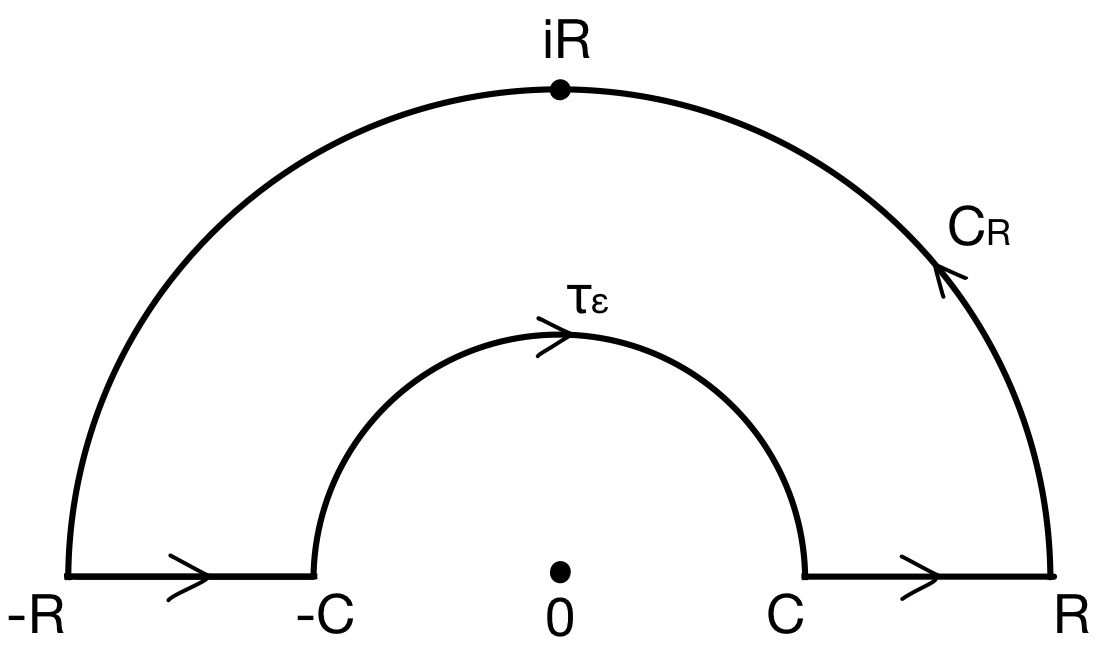
\includegraphics[scale=0.15]{21_5} 
\centering
\end{figure} 
Then $f$ is holomorphic on $C$'s interior and by Cauchy-Goursat Theorem, 
$$ 0 = \oint_Cf(z)\,dz = \int_{-R}^{-\varepsilon}f(z) \, dz + \int_{-\tau_\varepsilon}f(z) \, dz + \int_{\varepsilon}^{R}f(z) \, dz + \int_{C_R}f(z) \, dz$$
By Jordan's Lemma, 
$$\int_{C_R}f(z) \,dz \to 0 \text{ as } R\to \infty$$
By Semicircle Lemma, 
$$\int_{-\tau_\varepsilon}f(z) \, dz \to -\pi i \, Res(f, 0)$$
when $\varepsilon \to 0^+$ because there is a simple pole at 0. Therefore, 
\begin{align*}
&\int_{-R}^{-\varepsilon}f(z) \, dz + \int_{\varepsilon}^{R}f(z) \, dz = \int_{\tau_\varepsilon}f(z) \, dz = \pi i \, Res(f, 0) \text{ as } R \to \infty \text{ and } \varepsilon \to 0+ \\
\Rightarrow &P.V.\int_{\mathbb{R}}\frac{e^{ix}}{x} \, dx = \pi i \, Res(f, 0) = \pi i e^{iz} \bigg\rvert_{z = 0} = \pi i
\end{align*}
\newline
\textbf{Example.} Find 
$I = \int_0^{\infty} \frac{\sqrt{x}}{x^2 + 1} \, dx$
where $\sqrt{x} > 0$.
$$ I = \lim_{R \to \infty, \varepsilon \to 0^+} \int_{\varepsilon}^R \frac{\sqrt{x}}{x^2 + 1} \, dx$$ 
In this case, we need a contour in $\mathbb{C}$ that does the following: 
\begin{enumerate}[leftmargin=*, nolistsep]
\item $f$ is holomorphic in its interior.
\item The contour coincides with $\mathbb{R}^+$ for $f(z) = \frac{\sqrt{z}}{z^2 + 1}$. 
\item Avoid 0, the branch point. 
\end{enumerate}
\begin{figure}[h]
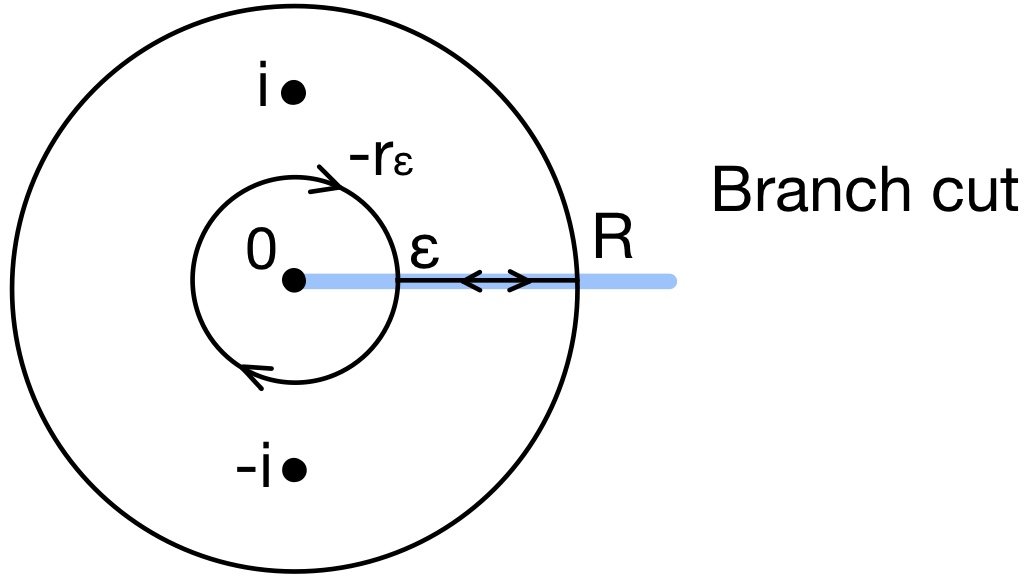
\includegraphics[scale=0.15]{21_6} 
\centering
\end{figure} 
This means the branch cut for $\sqrt{z}$ must be along $\mathbb{R}^+$. Else, $f$ is not meromorphic on the interior of $C$. 
\begin{align*}
\sqrt{z} &= e^{\frac{\operatorname{Log}|z| + i\theta}{2}}, \theta \in (0, 2\pi) \\
\oint_Cf(z) \,dz &= 2\pi i\left(Res(f, i) + Res(f, -1)\right) \\
&= \int_{\varepsilon}^{R}f(z) \,dz + \int_{C_R}f(z) \,dz + \int_{R}^{\varepsilon} f(z) \,dz + \int_{-\tau_\varepsilon} f(z) \, dz
\end{align*}
Now along the branch cut, we need to study the sign of $\sqrt{x}$. 
\begin{figure}[h]
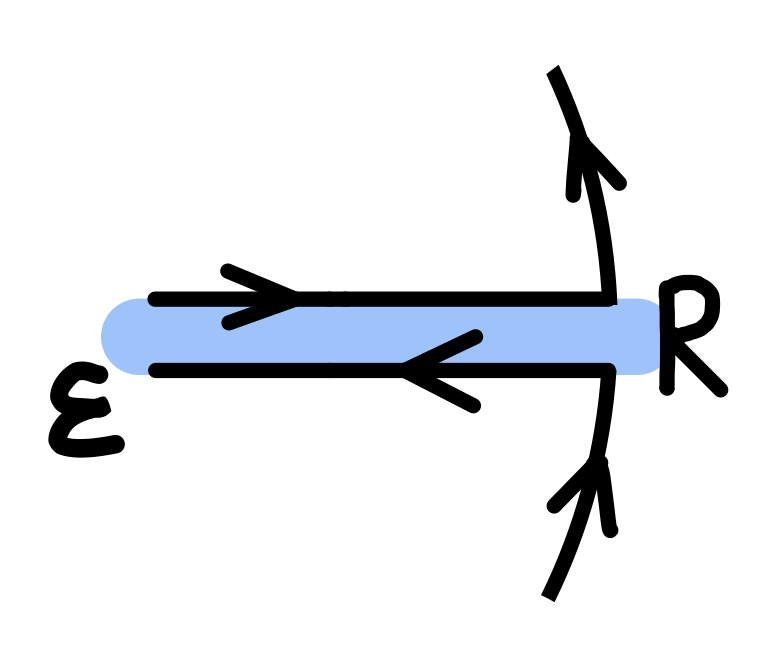
\includegraphics[scale=0.08]{21_7} 
\centering
\end{figure} 
On $[\varepsilon, R]$ and $[R, \varepsilon]$, we are using different branches of $\sqrt{z}$ but the same branch cut. \\
For $ y > 0$ and $x \in (\varepsilon, R)$, $\sqrt{x} > 0$. \\
For $ y < 0$ and $x \in (\varepsilon, R)$, $\sqrt{x} < 0$. 
\begin{align*}
\int_{\varepsilon}^{R} f(z) \, dz &= \int_{\varepsilon}^R \frac{\sqrt{z}}{z^2 + 1} \, dz \\
-\int_{R}^{\varepsilon}f(z) \, dz &= \int_{R}^{\varepsilon} \frac{-\sqrt{z}}{z^2 + 1}\,dz = \int_{\varepsilon}^{R}\frac{\sqrt{z}}{z^2 + 1}
\end{align*}
because $\varepsilon < R$. Therefore, 
$$ 2\int_{\varepsilon}^R \frac{\sqrt{z}}{z^2 + 1} \, dz = \int_{\varepsilon}^R f(z) \, dz - \int_{R}^{\varepsilon} f(z) \, dz$$
Now 
$$\abs*{\int_{C_R}f(z)\, dz} \leqslant 2\pi R \, \frac{A\sqrt{R}}{R^2} \to 0 \text{ as } R \to \infty$$ 
Observe for $\varepsilon \in (0, 1)$, 
$$ 1 - \varepsilon^2 \leqslant |\varepsilon^2 + 1| = \varepsilon^2 + 1 \Rightarrow \frac{1}{|\varepsilon^2 + 1|} \leqslant \frac{1}{1 - \varepsilon^2}$$
And so by an ML-Estimate, 
$$\abs*{\int_{-\tau_\varepsilon}f(z) \, dz} \leqslant \underbrace{\frac{\varepsilon^{\frac{1}{2}}}{1 - \varepsilon^2}}_{M} \, \underbrace{2\pi \varepsilon}_{L} \to 0 \text{ as } \varepsilon \to 0^+$$
As $\varepsilon \to 0^+, R \to \infty$, 
$$ 2I = 2\int_0^{\infty}\frac{\sqrt{x}}{x^2 + 1}\,dx = 2\pi i \, (Res(f, i) + Res(f, -i)) $$
The residues require us to use our branch of $\sqrt{z}, \operatorname{arg}(z) \in (0, 2\pi)$. 
\begin{align*}
Res(f, i) &= \frac{e^{\frac{\left(\operatorname{Log}|z| + i\operatorname{arg}(z)\right)}{2}}}{z + i} \Bigg\rvert_{z = i} \\
&= \frac{e^{\frac{0 + i\frac{\pi}{2}}{2i}}}{2i} \\
&= \frac{e^{i\frac{\pi}{4}}}{2i} \\
&= \frac{1}{2i}\left(\frac{\sqrt{2}}{2} + i\frac{\sqrt{2}}{2}\right) \\
& \\
Res(f, -i) &= \frac{e^{\frac{\left(\operatorname{Log}|z| + i\operatorname{arg}(z)\right)}{2}}}{z - i} \Bigg\rvert_{z = -i} \\
&= \frac{e^{\frac{0 + i\frac{3\pi}{2}}{2i}}}{-2i} \\
&= \frac{e^{i\frac{3\pi}{4}}}{-2i} \\
&= -\frac{1}{2i}\left(-\frac{\sqrt{2}}{2} + i\frac{\sqrt{2}}{2}\right) \\
& \\
\Rightarrow I &= \int_{0}^{\infty} \frac{\sqrt{x}}{x^2 + 1} \, dx \\
&= \pi i \left(\frac{1}{2i}\left(\frac{\sqrt{2}}{2} + i\frac{\sqrt{2}}{2}\right) - \frac{1}{2i}\left(-\frac{\sqrt{2}}{2} + i\frac{\sqrt{2}}{2}\right)\right) \\ 
&= \frac{\pi}{\sqrt{2}}
\end{align*}

\newpage
\section{Argument Principle and Rouche's Theorem}
Let $\gamma$ be a simple, piecewise smooth, closed curve in $\mathbb{C}$ oriented counter-clockwise. Let $f$ be meromorphic inside and on $\gamma$ but with no poles or zeros on $\gamma$.
\begin{figure}[h]
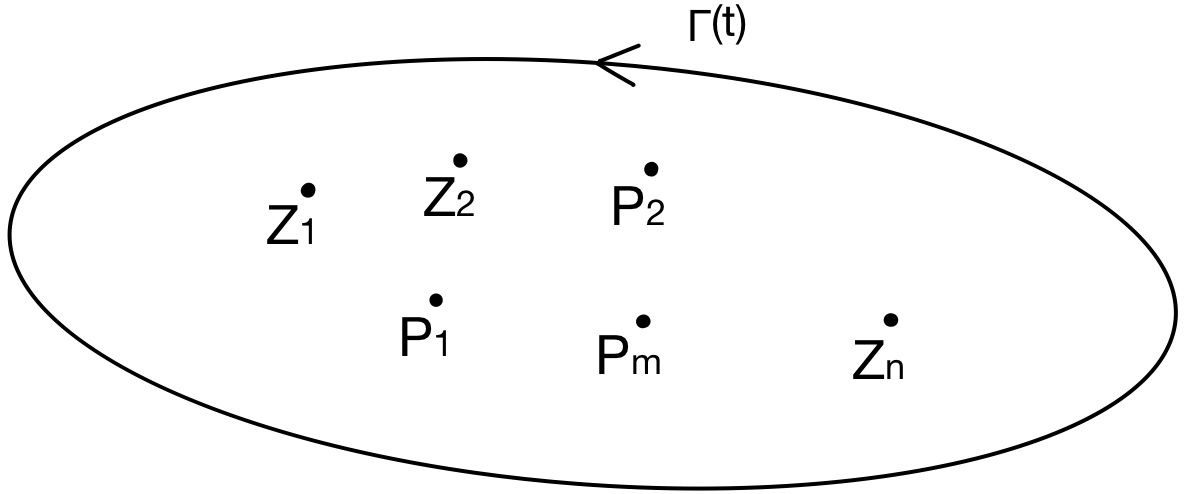
\includegraphics[scale=0.15]{22_1} 
\centering
\end{figure} 
\\
Let $p_1, p_2, \cdots, p_m$ be $f$'s poles in $\gamma$ and $z_1, \cdots, z_n$ be $f$'s zeros in $\gamma$. \\
Define $mult(z_k)$ and $mult(p_k)$ as the orders of the root $z_k$ and pole $p_k$. \\
Define 
\begin{align*}
Z_{f, \gamma} &= \sum mult(z_k) \\
P_{f, \gamma} &= \sum mult(p_k) 
\end{align*}
as the sum of the orders of the poles and roots of $f$ in $\gamma$. \\
\newline
\textbf{Lemma.} \\
With $f$ and $\gamma$ defined as above:
$$ \oint_{\gamma}\frac{f'(z)}{f(z)}\, dz = 2\pi i\,\left(\sum mult(z_k) - \sum mult(p_k)\right) = 2\pi i (Z_{f, \gamma} - P_{f, \gamma}) $$
\textbf{Proof.} Let $f$ have a zero of order $k$ at $z_0$. \\
\begin{align*}
&f(z) = (z - z_0)^kg(z), g(z_0) \neq 0 \\ 
\Rightarrow &f'(z) = (z - z_0)^{k - 1}\left(kg(z) + (z - z_0)g'(z_0)\right) \\ 
\Rightarrow & f' \text{ has a root of order } k - 1 \text{ at } z_0 \\
\Rightarrow & \frac{f'}{f} = \underbrace{\frac{k}{z - z_0}}_{\text{Singular Part}} + \underbrace{\frac{g'(z)}{g(z)}}_{\text{Holomorphic Part}}
\end{align*} 
Therefore, $\frac{f'}{f}$ has a simple pole and $Res(\frac{f'}{f}, z_0) = k$, which is also the order of the root at $z_0$ of $f$. \\
Repeat the argument with a pole at $p_0$ of order $k$, we have 
$$ \frac{f'}{f} = \frac{-k}{z - p_0} + \frac{g'(z)}{g(z)} $$
The result then follows by the Residue Theorem. 
\newpage
\textbf{Example.} Consider
$$\oint_{|z| = 4} \frac{f'(z)}{f(z)} \, dz \, \text{ for } \, f(z) = \frac{(z^2 + 1)^2}{(z^2 + 2z + 2)^3} $$
$f$ has ``4" roots in $|z| < 2$ and ``6" poles in $|z| < 4$. Therefore, 
$$\oint_{|z| = 4}\frac{f'(z)}{f(z)}\,dz = 2\pi i(4 - 6) = -4\pi i$$
\newline
\textbf{Example.} Consider 
$$ f(z) = z^5 - 3i z + 2z - 1 + i$$
$f(z)$ has 5 roots in $\mathbb{C}$ and 
$$ \oint_{|z| = R}\frac{f'(z)}{f(z)} \, dz = 2\pi i(5) = 10\pi i$$ 
for $R = \max|z_i|$ where $f(z_i) = 0$. \\
\newline
\textbf{Winding Number (Index).} \\
For any closed curve $\gamma$ in $\mathbb{C}$, its winding number (index) about $z_0$ is 
$$ Ind(\gamma, z_0) = \frac{1}{2\pi i}\oint_\gamma \frac{1}{z - z_0} \, dz \in \mathbb{Z}$$
If $\gamma$ is simple, then $Ind(\gamma, z_0) \in \{1, 0, -1\}$. \\
\newline
\textbf{Example.} 
\begin{align*}
	Ind(\gamma_1, z_0) &= 1 \\
	Ind(\gamma_2, z_0) &= -1 \\
	Ind(\gamma_3, z_0) &= 0 \\
\end{align*}
\begin{figure}[H]
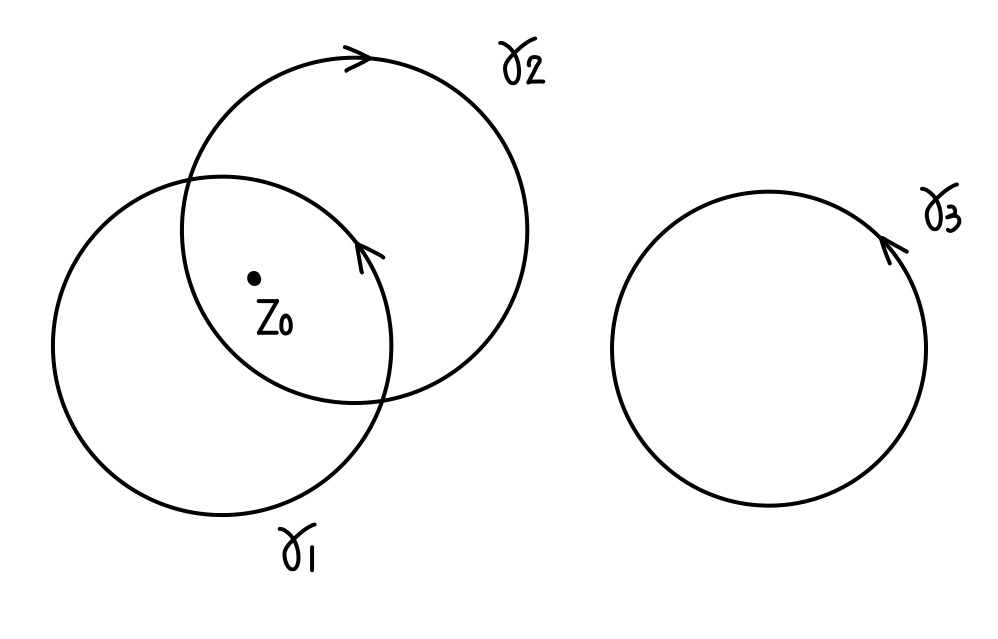
\includegraphics[scale=0.2]{22_4}
\centering
\end{figure} 
\iffalse
\begin{minipage}{.5\textwidth}
       \begin{align*}
	Ind(\gamma_1, z_0) &= 1 \\
	Ind(\gamma_2, z_0) &= -1 \\
	Ind(\gamma_3, z_0) &= 0 \\
	\end{align*}
  \end{minipage}%
  \begin{minipage}{.5\textwidth}
    \centering
    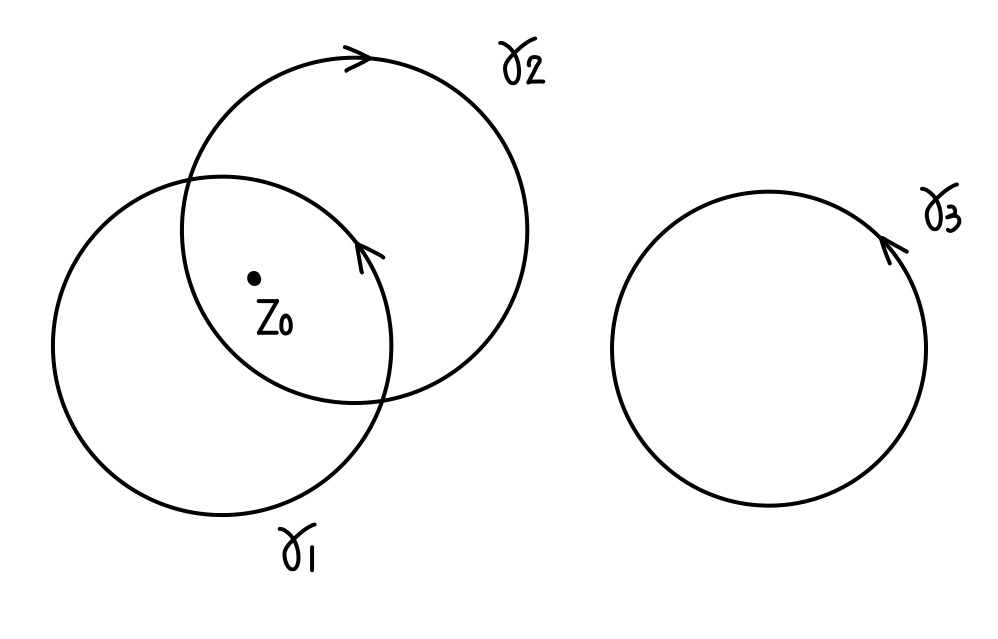
\includegraphics[scale = 0.2]{22_4}
\end{minipage} 

\begin{figure}[H]
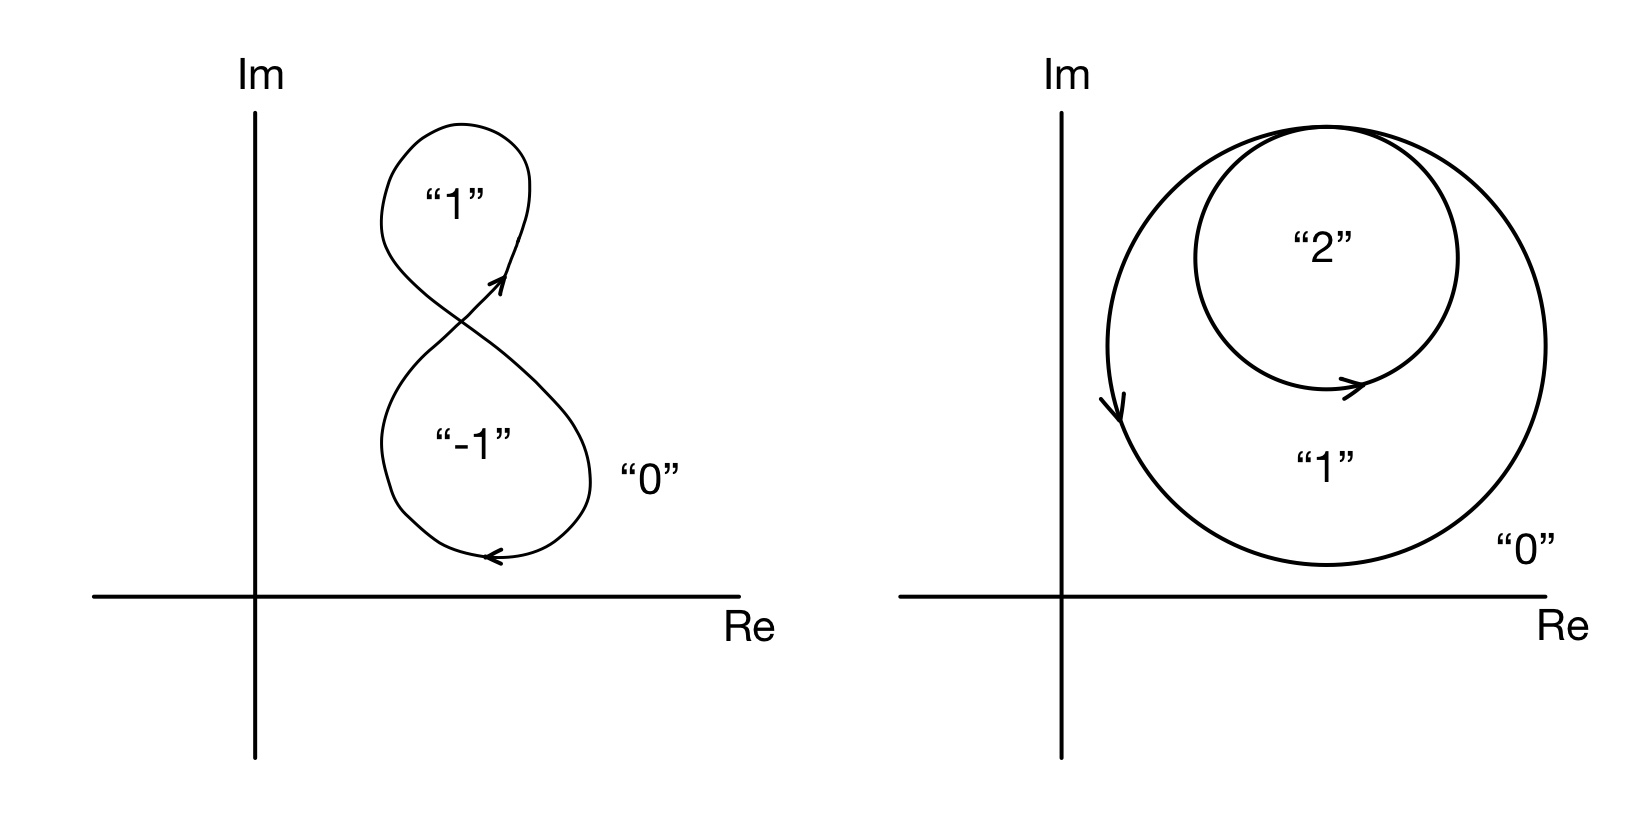
\includegraphics[scale=0.2]{22_2}
\centering
\end{figure} 
\begin{figure}[H]
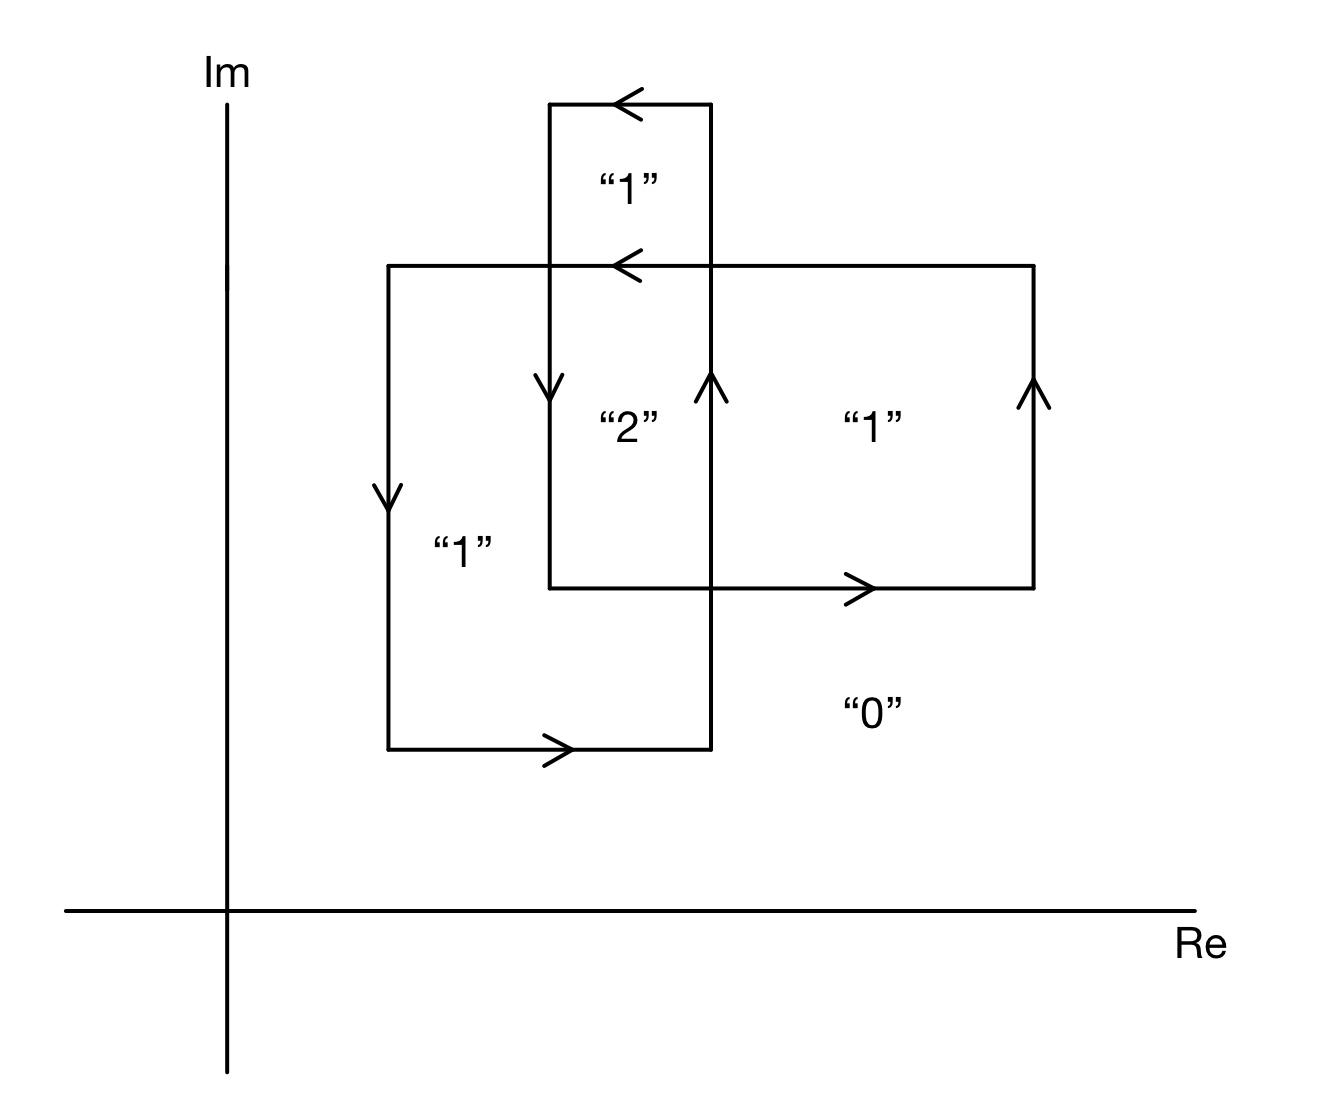
\includegraphics[scale=0.17]{22_3} 
\centering
\end{figure}
\fi
\begin{figure}[H]
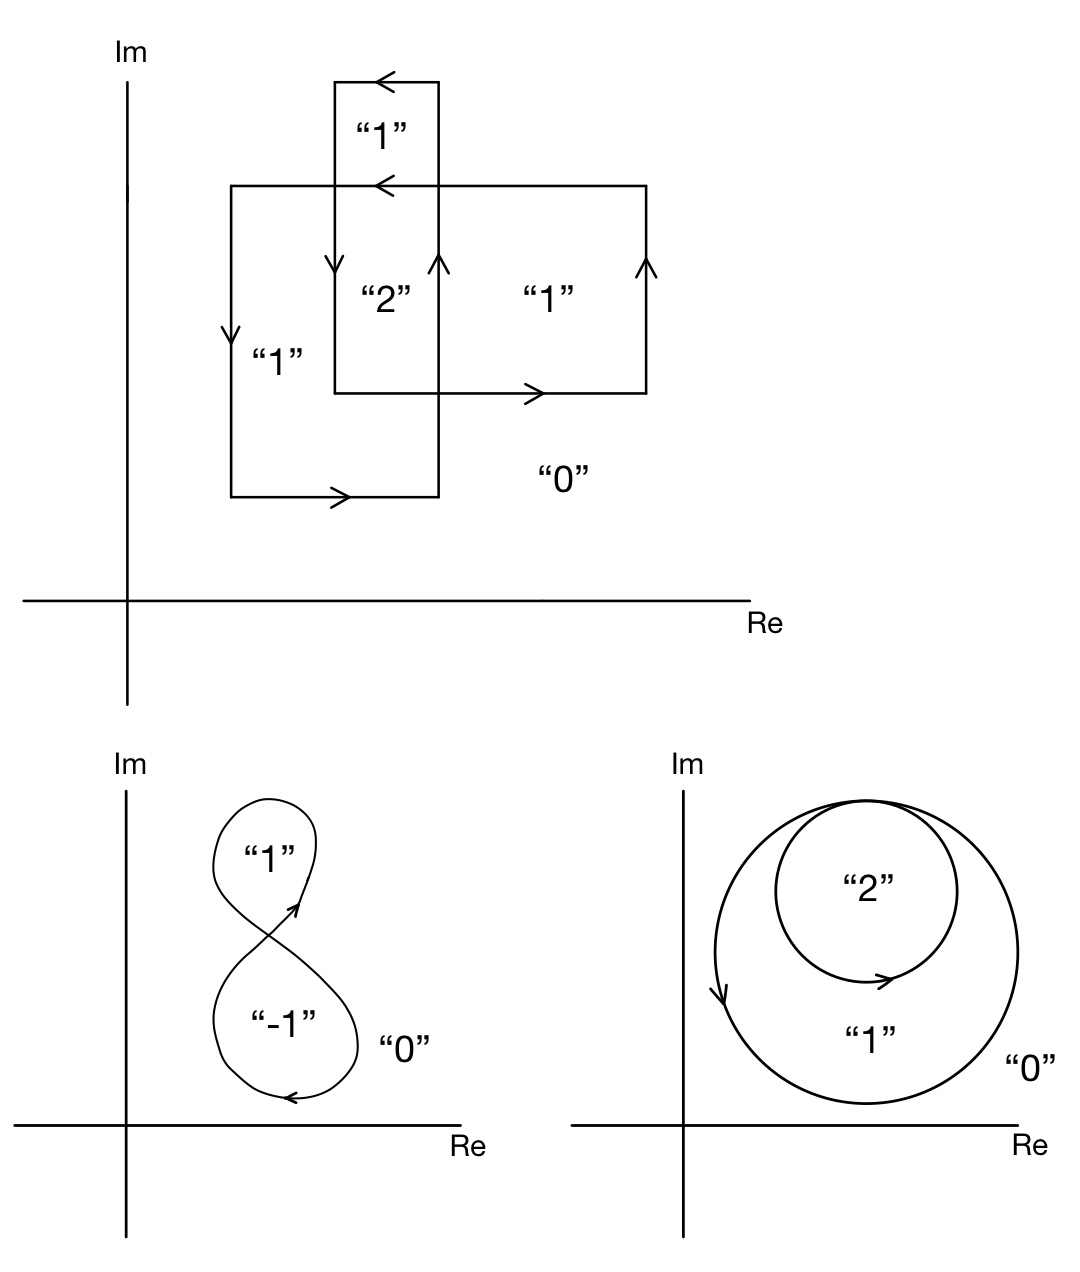
\includegraphics[scale=0.23]{22_23} 
\centering
\end{figure}
\textbf{Example.} \\
If $\gamma_1(t) = e^{it}$ and $f_1(z) = z^2$, then $ f_1 \circ \gamma_1 = e^{2it}$ traverses the unit circle twice for $t \in [0, 2\pi]$. \\
Therefore, $Ind( f_1 \circ \gamma_1, 0) = 2$. 
\begin{figure}[H]
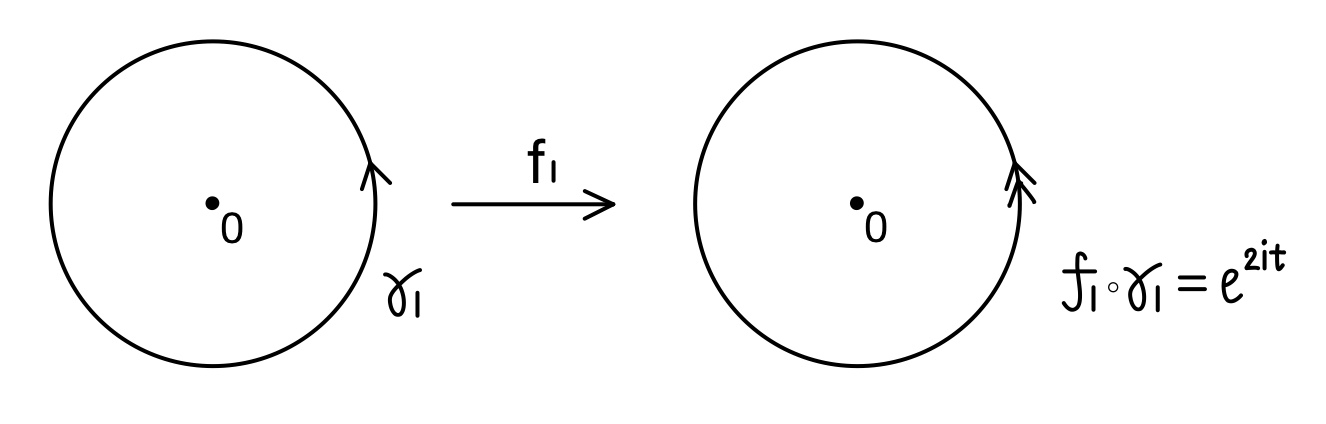
\includegraphics[scale = 0.18]{22_5}
\centering
\end{figure}
If $\gamma_2(t) = it, t \in \mathbb{R}$ and $f_2 = \frac{1}{z + 1}$, then $f_2 \circ \gamma_2$ is a circle about $\frac{1}{2}$ of radius $\frac{1}{2}$ by the Möbius transform theory. \\
Therefore, $Ind( f_2 \circ \gamma_2, \frac{1}{2}) = -1$. 
\begin{figure}[H]
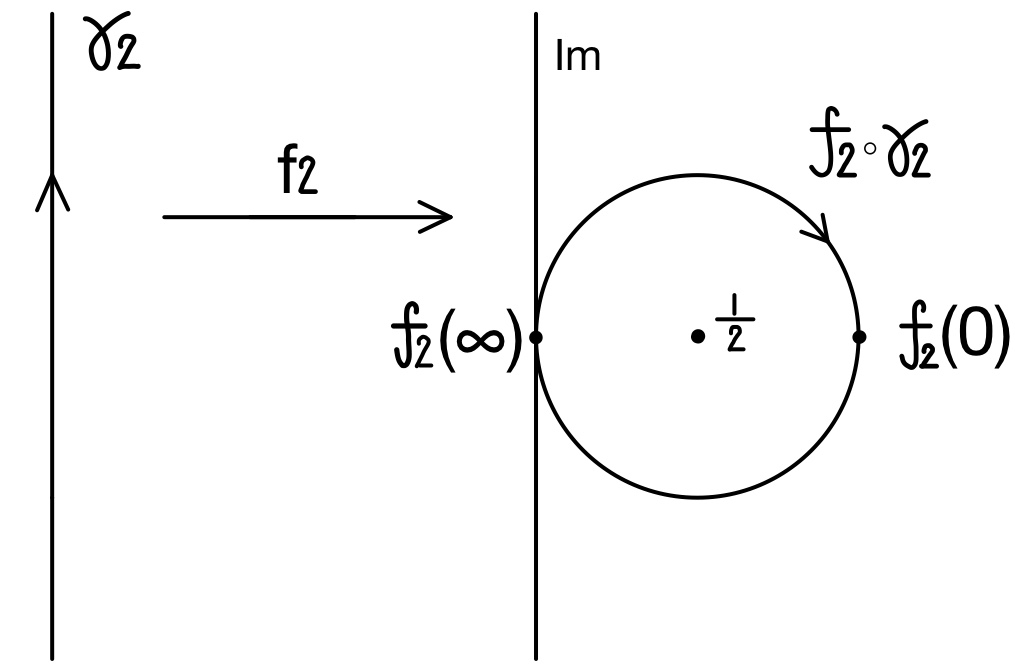
\includegraphics[scale = 0.17]{22_6}
\centering
\end{figure}
The number of times $f \circ \gamma$ wraps around $w_0$ implies how many solutions exist to $f(z) = w_0$ for $z$ inside $\gamma$. \\
\newline
\textbf{Argument Principle. } \\
For $f$ and $\gamma$ as in our lemma, 
$$ \oint_{\gamma}\frac{f'(z)}{f(z)} \,dz = 2\pi i \, Ind(f\circ \gamma, 0) = 2\pi i(Z_{f, \gamma} - P_{f, \gamma})$$
\textbf{Proof.} Let $w = f(z)$, then $z = \gamma(t)$. Then, $w = f \circ \gamma$ and $dw = f'(z) \, dz$. 
$$ \oint_\gamma \frac{f'(z)}{f(z)} \,dz = \int_{f\circ \gamma}\frac{dw}{w} = 2\pi i\, Ind(f\circ \gamma, 0) = 2\pi i(Z_{f, \gamma} - P_{f, \gamma}) $$
We can measure how many times a curve in $\mathbb{C}$ is wrapped around a point in the $w$=plane by $w = f(z)$ or measure the change in the curve's argument. 
$$ \oint_{\gamma}\frac{f'}{f}\,dz = \frac{1}{2\pi i} \operatorname{Log}\left(f(z)\right)\Bigg\rvert_{z = \gamma(0)}^{\gamma(1)} = \frac{1}{2\pi} \bigtriangleup \operatorname{Arg}\left(f(z)\right)$$
for $\gamma(0) = \gamma(1)$. (The $\mathbb{R}$-part vanishes since $|f(\gamma(0))| = |f(\gamma(1))|$). \\
\begin{figure}[H]
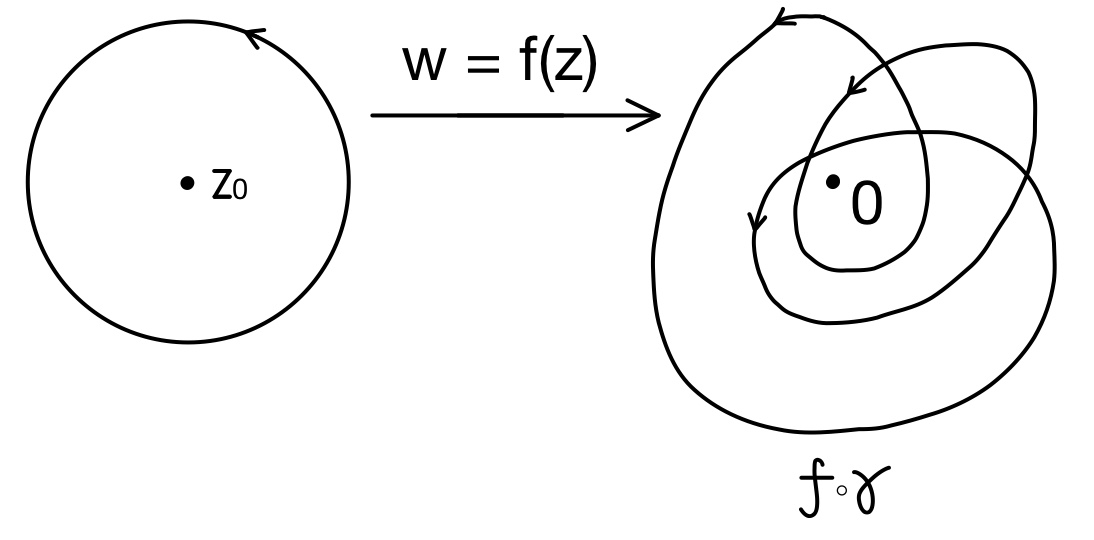
\includegraphics[scale = 0.17]{22_7}
\centering
\end{figure}
\textbf{Example.} Let $f(z) = z^2 + z$. It has two roots 0 and -1 and no poles. \\
Let $\gamma_1$ be a circle of radius 2, and both roots are inside $f \circ \gamma_1$. Therefore, $Ind(f \circ \gamma_1, 0) = 2$. \\
\begin{figure}[H]
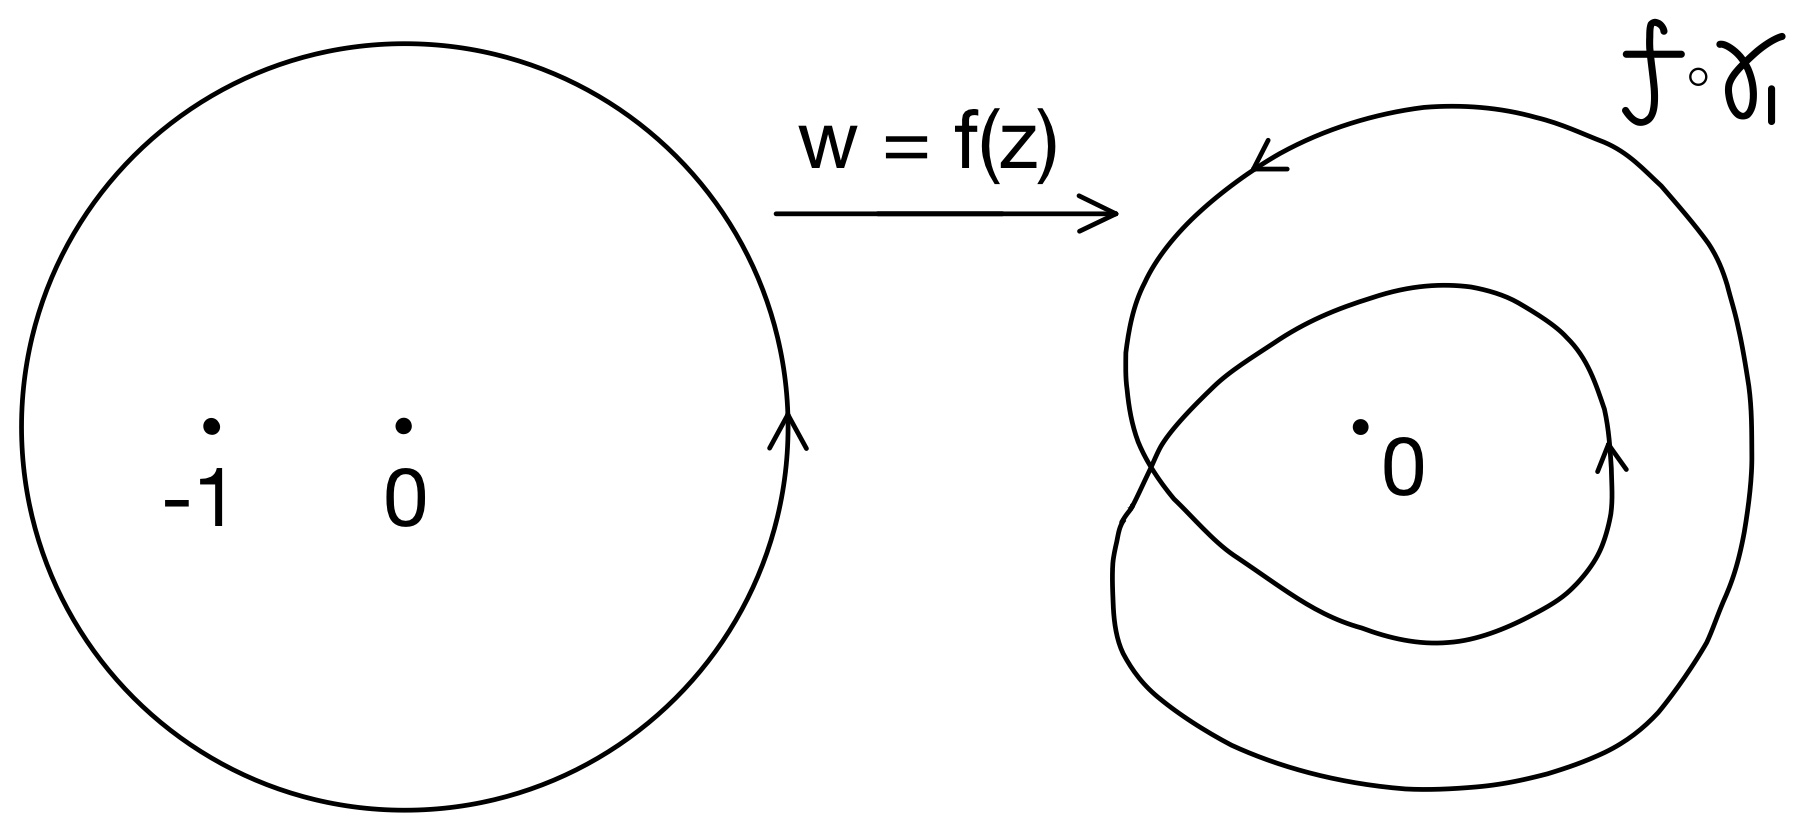
\includegraphics[scale = 0.14]{22_8}
\centering
\end{figure}
Let $\gamma_2$ be a circle of radius $\frac{1}{2}$, and one root is inside $f \circ \gamma_2$. Therefore, $Ind(f \circ \gamma_2, 0) = 1$. \\ 
\begin{figure}[H]
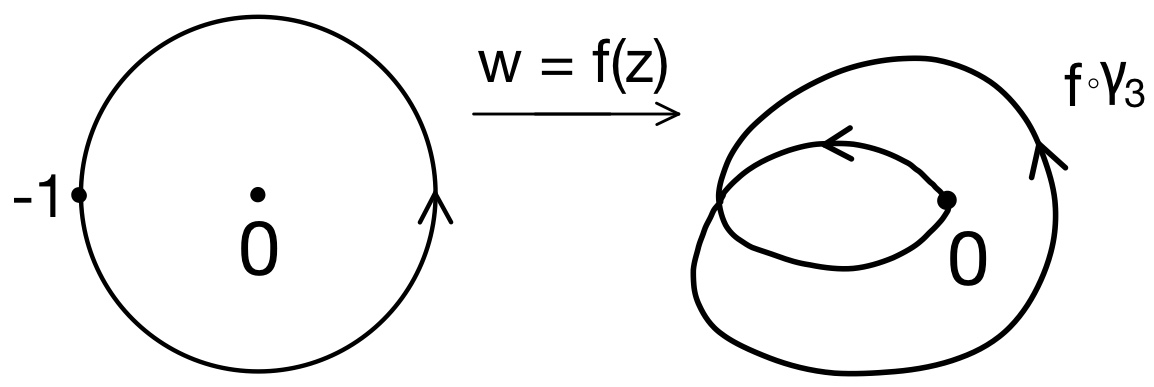
\includegraphics[scale = 0.2]{22_9}
\centering
\end{figure}
Let $\gamma_3$ be a circle of radius 1, and it passes through the root -1. Therefore, the Argument Principle fails. \\ 
\begin{figure}[H]
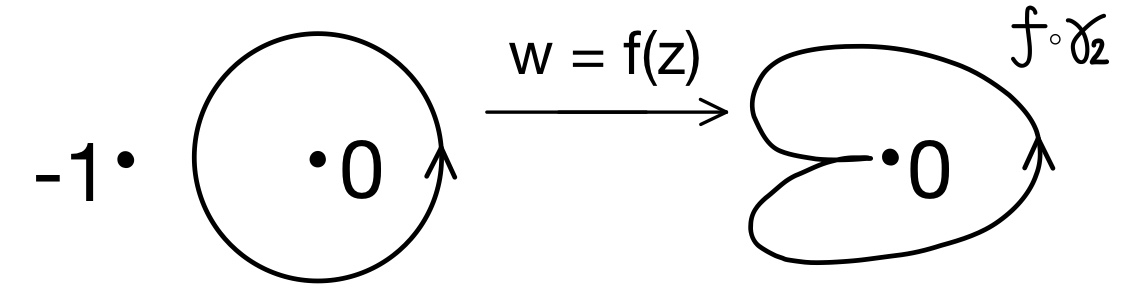
\includegraphics[scale = 0.2]{22_10}
\centering
\end{figure}
Imagine you are always 10 feet or more from a tree and you are walking a dog with an 8 feet leash. Everything you walk around the tree, so must the dog. \\ 
Let $f$ be a function and $|h| < |f|$, then the perturbed function $f + h$ has its roots near the roots of $f$. Here $h$ is a ``small" change to $f$. \\
\newline
\textbf{Rouche's Theorem.} \\
Let $\gamma$ be simple closed curve in $\mathbb{C}$. Suppose $f$ and $h$ are meromorphic inside and on $\gamma$, but with no poles on $\gamma$, and $|h| < |f|$ on $\gamma$. Then 
$$ Z_{f, \gamma} - P_{f, \gamma} = Z_{f + h, \gamma} - P_{f + h, \gamma} $$
\textbf{Proof.} \\
Claim 1: $f$, $f + h$ and $\frac{f + h}{f}$ have no roots on $\gamma$. 
\begin{align*}
0 \leqslant |h| < |f| &\Rightarrow f \text{ has no roots on } \gamma \\
&\Rightarrow f + h \text{ has no roots on } \gamma \text{, since } |h| - |f| \neq 0 \text{ on } \gamma \\
&\Rightarrow \frac{f + h}{f} \text{ has no roots on } \gamma \text{ since } f + h \neq 0 \text{ on } \gamma
\end{align*}
Claim 2: $f$, $f + h$ and $\frac{f + h}{f}$ have no poles on $\gamma$. \\
$f$ and $f + h$ have no poles by our hypothesis and $f \neq 0$ on $\gamma$. Therefore, $\frac{f + h}{f}$ has no poles on $\gamma$. \\
By the Argument Principle, 
\begin{align*}
\oint_{\gamma} \frac{f'}{f} \, dz &= 2 \pi i\,Ind(f\circ \gamma, 0) = 2\pi i( Z_{f, \gamma} - P_{f, \gamma}) \\
\oint_{\gamma} \frac{f' + h'}{f + h} \, dz &= 2\pi i\, Ind\left((f + h) \circ \gamma, 0\right) = 2\pi i(Z_{f + h, \gamma} - P_{f + h, \gamma})
\end{align*}
Now $\abs*{\frac{h}{f}} < 1$ and so $\frac{h}{f} \circ \gamma$ is in the unit circle. \\
Then $g = 1 + \frac{h}{f}$ maps $\gamma$ to the interior of a circle centered at 1 with radius 1. \\
\begin{figure}[H]
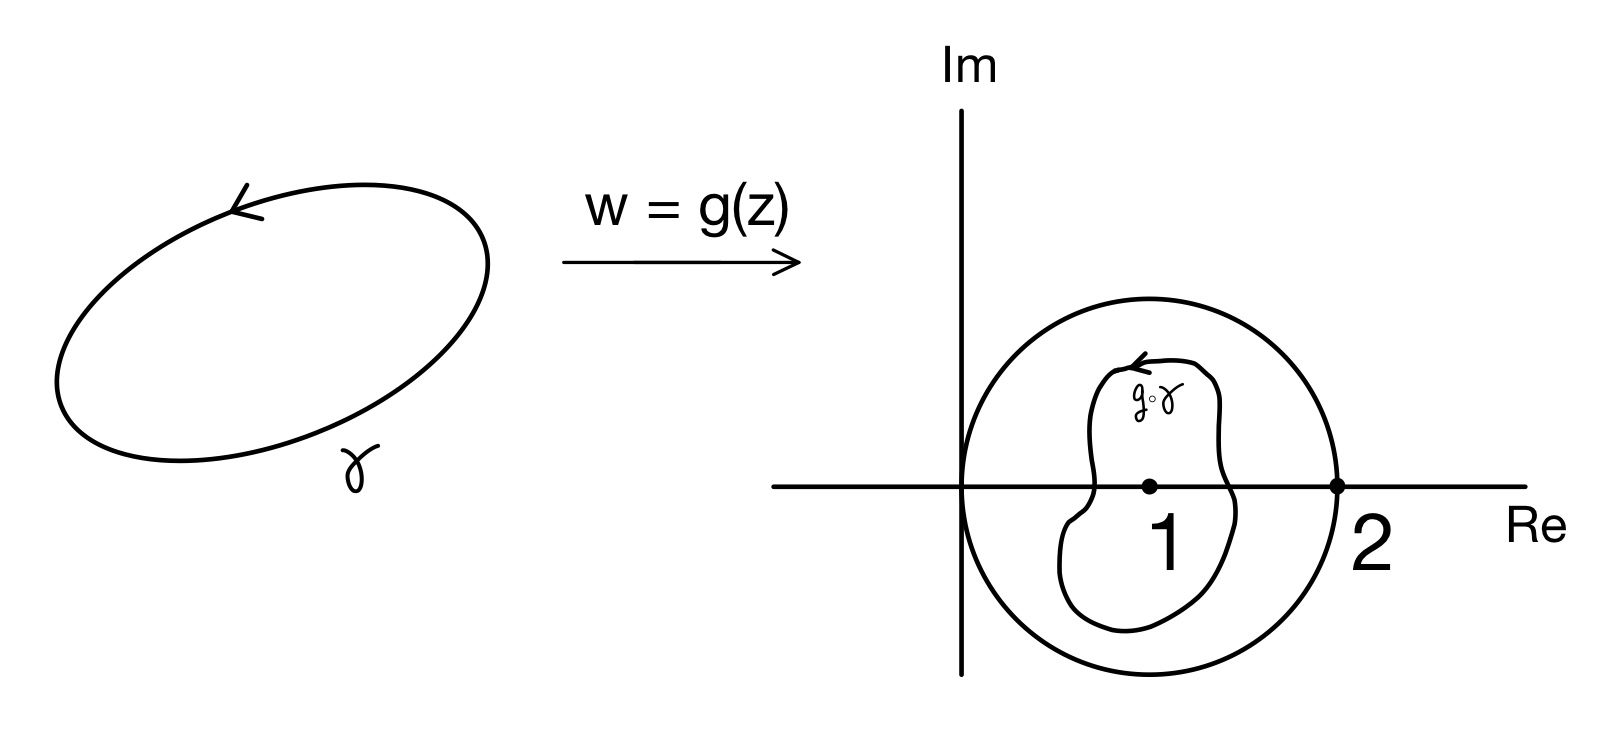
\includegraphics[scale = 0.18]{22_11}
\centering
\end{figure}
Since the curve cannot contain 0, $Ind(g, 0) = 0$. Then, 
\begin{align*}
&\hspace{5mm} \frac{g'}{g} = \frac{f' + h'}{f + h} - \frac{f'}{f} \\
&\Rightarrow 0 = \oint_\gamma \frac{g'}{g} \, dz \\ 
&\Rightarrow = \oint_\gamma \frac{f' + h'}{f + h} \, dz - \oint_\gamma \frac{f'}{f} \, dz \\
&\Rightarrow Ind(f + h, 0) = Ind(f, 0)
\end{align*}
\newline
\textbf{Corollary.} \\
If $f$ and $g$ are also holomorphic inside and on $\gamma$, then 
$$ Z_{f, \gamma} = Z_{f + h, \gamma} $$
Rouche's Theorem gives us an easy way to locate roots. \\
\newline
\textbf{Example.} Locate the roots of $\alpha(z) = z + 3 + 2e^z$. \\
Let $f = z + 3$ and $h = 2e^z$ so that $\alpha = f + h$. For $R$ large, we want $|f| > |h|$ on $C_R$ and $C_1$, a contour similar to one seen before. 
\begin{figure}[H]
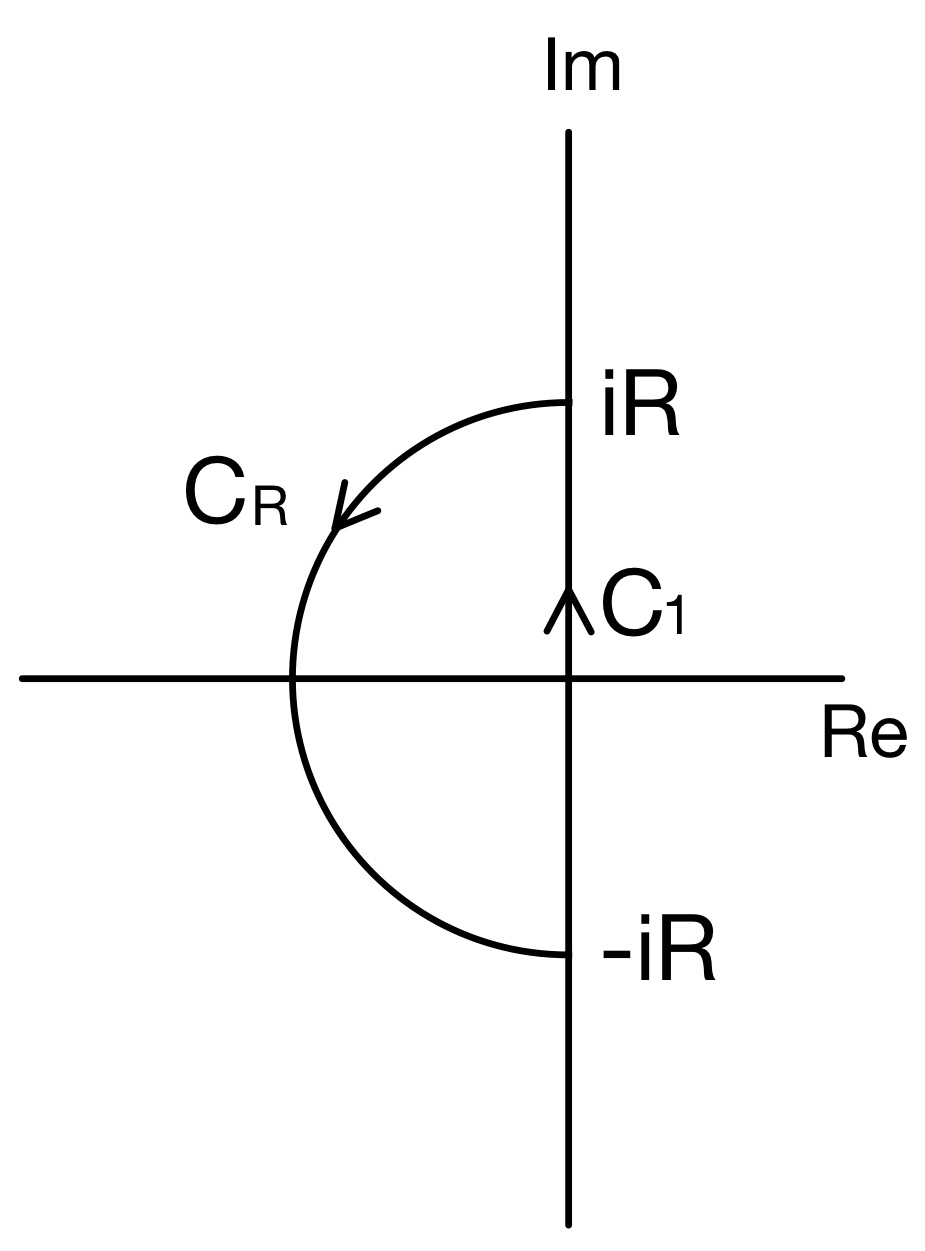
\includegraphics[scale = 0.15]{22_12}
\centering
\end{figure}
If $z \in C_1, z = iy$. 
\begin{align*}
|f(z)| &= | 3+iy| > 3 \\
|h(z)| &= 2|e^{iy}| = 2
\end{align*} 
Hence, $|h| < |f| $ on $C_1$. For $z \in C_R, z = x + iy, |z| = R$ and $x < 0$, 
\begin{align*}
&|f(z)| > R - 3 \text{ for } R \text{-large} \\
&|h(z)| = 2\abs*{e^{x + iy}} = 2e^x < 2 \text{ because } x < 0 \\ 
\Rightarrow \hspace{2mm} & |h| < |f| \text{ on } C \text{ and } f(z) = 3 + z \text{ has only one root for all } R \text{ large} \\
\Rightarrow \hspace{2mm} & \alpha \text{ has only one root in } \Re(z) < 0.
\end{align*}
\textbf{Example.} Find how many roots $2z^{10} + 4z^2 + 1$ has in $|z| < 1$. \\
On $|z| = 1$, let $f = 4z^2$ and $h = 2z^{10} + 1$, $ |f| > |h|$. Therefore, $f + h = 2z^{10} + 4z^2 + 1$ have exactly two roots in $|z| < 1$. \\
\newline
\textbf{Example.} Let $\frac{1}{3}e^z - z = 0$. Does it have a solution in $|z| < 1$? \\
Observe $|z| > \abs*{\frac{1}{3}e^z}$ for $|z| = 1$ and $f(z) = -z$ has one root in $|z| < 1$. Therefore, $f + \abs*{\frac{1}{3}e^z}$ has exactly one root in $|z| < 1$.\\
\newline
\textbf{Example.} Locate the roots of $\alpha(z) = z^7 - 5z^3 + 12$. \\
On $|z| = 1$, let $f = 12$, $h = z^7 - 5z^3$. $|f| = 12$ and $|h| \leqslant |1| + |5| = 6 < 12$. Since $f$ does not have a root on $|z| < 1$, $f + h = \alpha$ has no roots in $|z| < 1$. \\
On $|z| = 2$, let $f = z^7$, $h = -5z^3 + 12$. $|f| = 2^7 = 128, |h| \leqslant 5|z|^3 +12 = 52$. So on $f$ and $f + h$ have the same number of roots on $|z| < 2$, which is 7. \\
Therefore, all of $\alpha$'s 7 roots are in $1 < |z| < 2$. \\
\newline
\textbf{Corollary: Fundamental Theorem of Algebra. } \\
Let $\alpha(z) = z^n + a_{n - 1}z^{n - 1} + \cdots + a_0$ and $f(z) = z^n$. \\
Let $h(z) = \alpha(z) - f(z) \Rightarrow f + h = \alpha$ \\
Let $R = \max \{1, n|a_{n - 1}|, \cdots, n|a_0|\} + 1$, then on $|z| = R$ 
\begin{align*}
|h| &\leqslant |a_{n - 1}|R^{n - 1} +  |a_{n - 2}|R^{n - 2} + \cdots + |a_0| \\
&\leqslant \frac{R}{n}R^{n - 1} + \frac{R}{n}R^{n - 2} + \cdots + |a_0| \\
&\leqslant \underbrace{\frac{R^n}{n} + \frac{R^n}{n} + \cdots + \frac{R^n}{n}}_{\text{n-terms}} \\
&= R^n
\end{align*}
On $|z| = R, |f(z)| = R^n \Rightarrow |h| < |f|$ for $|z| = R$. \\
Then $f + h$ and $f$ have the same number of zeros on $|z| < R$, $n$, by Rouche's Theorem. As $R \to \infty$, we have exactly $n$ roots in $\mathbb{C}$. 
\newpage
\end{document}